\documentclass[twoside,a4paper]{report}  
\usepackage{a4}
% Not needed, since our text is english:
%\usepackage{t1enc}
\usepackage{epsf}
\usepackage{latexsym}
\usepackage{amssymb}
\usepackage[dvips]{graphicx}
\usepackage{makeidx}
\usepackage{textcomp}
\usepackage{marvosym}
\usepackage{tabularx}
\usepackage{longtable}
\usepackage{calc}

\usepackage{color}
\definecolor{linkblue}{rgb}{0, 0, 0.5}
\definecolor{urlblue}{rgb}{0, 0, 1}
\definecolor{citegreen}{rgb}{0, 0.4, 0}

\usepackage[ bookmarks=true,%
  bookmarksnumbered=true,%
  breaklinks=true,%
  colorlinks=true,%
  linkcolor=linkblue,%
  urlcolor=urlblue,%
  citecolor=citegreen]{hyperref}

\hypersetup{
  pdfauthor   = {Juha Aatrokoski, Timo Lilja, Leena Salmela, Teemu J. Takanen, Aleksi Virtanen, Philip Meulengracht},
  pdftitle    = {User-guide to KUdos System},
  pdfsubject  = {Reference Manual},
}

%\frenchspacing

% use section for all levels with autoref:
\renewcommand{\subsectionautorefname}{section}
\renewcommand{\subsubsectionautorefname}{section}


% From the LaTeX companion, PreserveBackslash:
\newcommand{\PBS}[1]{\let\temp=\\#1\let\\=\temp}
\newlength{\tablewidth}


\newenvironment{function}[3]{%
\paragraph{\texttt{#1 {\textbf{#2}} (#3)}}%
\index{#2@\texttt{#2}}%
\begin{itemize}%
}{%
\end{itemize}%
}

\newcommand{\parameter}[3]{%
\paragraph{\texttt{#1}}%
\index{#1@\texttt{#1}}%
\begin{itemize}%
\item \textbf{Purpose:} #2%
\item \textbf{Value range:} #3%
\end{itemize}%
}


\newenvironment{structdescription}{%
\begin{center}%
\begin{tabular}{p{3.5cm}|p{2.5cm}|>{\PBS\raggedright}p{\tablewidth-6\tabcolsep-6cm}}%
\textbf{Type} & \textbf{Name} & \textbf{Explanation} \\ %
}{%
\end{tabular}%
\end{center}%
}

% Arguments are caption,label
\newenvironment{longstructdescription}[2]{%
\begin{center}%
\begin{longtable}{p{3.5cm}|p{2.5cm}|>{\PBS\raggedright}p{\tablewidth-6\tabcolsep-6cm}}%
\multicolumn{3}{l}{\emph{Continued from the previous page}}\\%
\multicolumn{3}{l}{}\\%
\textbf{Type} & \textbf{Name} & \textbf{Explanation}%
\endhead%
\textbf{Type}\label{#2} & \textbf{Name} & \textbf{Explanation}\\%
\endfirsthead%
\multicolumn{3}{r}{}\\%
\multicolumn{3}{r}{\emph{Continued on the next page}}\\%
\multicolumn{3}{r}{}\\%
\caption{#1}%
\endfoot%
\multicolumn{3}{r}{}\\%
\caption{#1}%
\endlastfoot%
}{%
\end{longtable}%
\end{center}%
}

% For file formats etc. data structures. Use \formatfield for rows
\newenvironment{formatdescription}{%
\begin{center}%
\begin{tabular}{p{1.2cm}|p{2.8cm}|p{1.5cm}|>{\PBS\raggedright}p{\tablewidth-8\tabcolsep-5.5cm}}%
\textbf{Offset} & \textbf{Type} & \textbf{Name} & \textbf{Description} \\ %
}{%
\end{tabular}%
\end{center}%
}


\newcommand{\structfield}[3]{%
\hline%
\texttt{#1} & \texttt{#2} & #3 \\%
}

\newcommand{\formatfield}[4]{%
\hline%
\texttt{#1} & \texttt{#2} & \texttt{#3} & #4 \\%
}

\newcommand{\buenos}{\texttt{\textbf{BUENOS}}}
\newcommand{\kudos}{\texttt{\textbf{KUDOS}}}
\newcommand{\yams}{\texttt{\textbf{YAMS}}}

\newenvironment{filelist}[0]{%
\vspace{\baselineskip}%
\begin{center}%
\begin{tabular}{p{4cm}>{\PBS\raggedright}p{\tablewidth-4\tabcolsep-4cm}}%
\hline%
}{%
\end{tabular}%
\end{center}%
}

\newcommand{\file}[2]{\texttt{#1} \vspace{2mm} & #2 \vspace{2mm}\\}

\newcommand{\metavar}[1]{\textrm{\textsl{#1}}}

% Line break + indent for long function descriptions
\newcommand{\brtab}{\\\hspace*{1cm}}

% Optional preamble rgument, defaults to a numberless section
\newenvironment{exercises}[1][\addcontentsline{toc}{section}{Exercises}%
\section*{Exercises}\markright{EXERCISES}]{%
#1%
\begin{enumerate}%
}{%
\end{enumerate}
}

\newcounter{exercisec}[chapter]

% For normal exercises
\newcommand{\exercise}[1]{%
\item[\stepcounter{exercisec}\arabic{chapter}.\theexercisec{}.] #1%
}

% For exercises involving programming
\newcommand{\cexercise}[1]{%
\item[\stepcounter{exercisec}{\huge\Keyboard}\hspace{5mm}\textbf{\arabic{chapter}.\theexercisec{}.}] #1%
}


\newcommand{\ttilde}{\symbol{126}}

\makeindex


\newcommand{\authors}{%
Juha~Aatrokoski, Timo~Lilja, Leena~Salmela, %
Teemu~J.~Takanen, Aleksi~Virtanen and Philip Meulengracht%
}


% Page layout: move towards outer edge and add headers
%
\usepackage{fancyhdr}
\pagestyle{fancy}
\addtolength{\oddsidemargin}{0.5in}
\addtolength{\evensidemargin}{-0.5in}
% add two lines to the bottom
%\addtolength{\textheight}{\baselineskip}
% page number overhang by 1cm:
\addtolength{\headwidth}{0.5cm}
\fancyhf{}
\fancypagestyle{normal}{%
  \fancyhead[LE,RO]{\thepage}%
  \fancyhead[LO]{\slshape\rightmark}%
  \fancyhead[RE]{\slshape\leftmark}%
  \renewcommand{\headrulewidth}{0.5pt}%
}
\fancypagestyle{plain}{%
  \fancyhead{}%
  \renewcommand{\headrulewidth}{0pt}%
}


%\overfullrule=5pt
\emergencystretch=10pt

\begin{document}
\pagestyle{plain}
%\maketitle
%%%%%%%%%%%%%%%%%
% Titlepage in texinfo style
\begin{titlepage}
{
\vspace*{\stretch{1}}
\raggedright\bfseries\Huge
\texttt{KUDOS}\\
\large
\hspace{1em}is the\\
Koebenhavns Universitet Discrete Operating System\\
\rule{\textwidth}{2mm}
\raggedleft\bfseries\large
The roadmap of the \texttt{KUDOS} system\\
Version 1.0\\
\today\\
\vspace*{\stretch{2}}
\raggedright\bfseries\large
\authors{}\\
%\vspace{-2mm}
\rule{\textwidth}{1mm}
}
\newpage
\vspace*{\stretch{1}}
\noindent

\noindent\buenos{}/\kudos{} is licenced under the following "modified BSD
license" (i.e., the BSD license without the advertising clause).

\begin{flushleft}
\vspace{\baselineskip}
Copyright \copyright{} 2003--\number\year{} \authors{}
\vspace{\baselineskip}
\end{flushleft}

Redistribution and use in source and binary forms, with or without
modification, are permitted provided that the following conditions
are met:

\begin{enumerate}
\item Redistributions of source code must retain the above copyright
    notice, this list of conditions and the following disclaimer.
\item Redistributions in binary form must reproduce the above
    copyright notice, this list of conditions and the following
    disclaimer in the documentation and/or other materials provided
    with the distribution.
\item The name of the author may not be used to endorse or promote
    products derived from this software without specific prior
    written permission.
\end{enumerate}

THIS SOFTWARE IS PROVIDED BY THE AUTHOR ``AS IS'' AND ANY EXPRESS
OR IMPLIED WARRANTIES, INCLUDING, BUT NOT LIMITED TO, THE IMPLIED
WARRANTIES OF MERCHANTABILITY AND FITNESS FOR A PARTICULAR PURPOSE
ARE DISCLAIMED. IN NO EVENT SHALL THE AUTHOR BE LIABLE FOR ANY
DIRECT, INDIRECT, INCIDENTAL, SPECIAL, EXEMPLARY, OR CONSEQUENTIAL
DAMAGES (INCLUDING, BUT NOT LIMITED TO, PROCUREMENT OF SUBSTITUTE
GOODS OR SERVICES; LOSS OF USE, DATA, OR PROFITS; OR BUSINESS
INTERRUPTION) HOWEVER CAUSED AND ON ANY THEORY OF LIABILITY,
WHETHER IN CONTRACT, STRICT LIABILITY, OR TORT (INCLUDING
NEGLIGENCE OR OTHERWISE) ARISING IN ANY WAY OUT OF THE USE OF THIS
SOFTWARE, EVEN IF ADVISED OF THE POSSIBILITY OF SUCH DAMAGE.

\end{titlepage}
%%%%%%%%%%%%%%%%%


\tableofcontents

\cleardoublepage
\pagestyle{normal}
\pagenumbering{arabic}
\setlength{\tablewidth}{\linewidth-1cm}

\chapter{Introduction}

\kudos{} is a derivative project from \buenos{} which aside from supporting
the old \buenos{} system, now also supports the Intel x86-64 Architecture.
The new operating system, \kudos{}, is meant also meant as a exercise base
for the operating system course, but with a more common platform in mind.
Unlike its old project \buenos{}, \kudos{} will run on more recent real-world
hardware\footnote{In theory.} without any special architecture, but rather 
on your own laptop at home.

The system is kept structurally intact to \buenos{}, however all platform-specific
code has been split up into sub-directories, and is controlled with the makefile.
\kudos{} systems are ready for multi-core, however support for starting other
application processors has not been implemented, while the \buenos{} part
has the multi-core support. Both \buenos{} and \kudos{} also provides skeleton code 
for threading, wide variety of synchronization primitives, userland support and
proccesses.A simple custom filesystem and code for networking is also 
provided (However no network-card drivers are provided). 

To keep both 32 bit code (the mips project) and 64 bit code (the x86-64 project)
under the same roof, many modifications had to be made to the old \buenos{} 
project, and thus the structure of the project has changed partially. It has also
changed the procedure for starting up the new operating system, \kudos{}.

Just like \buenos{}, the main idea of the system is to give you a real, working
multiprocessor operating system kernel which is as small and simple as
possible. To boot \kudos{}-x86-64 on a real computer all you would need is simply
GRUB2 as a bootloader, and then make sure to add \kudos{} as a boot
entry into GRUB2. \kudos{} now supports your everyday intel 64 bit
architecture and thus can run on your everyday computer. No code
modifcations would be neccessary. 


\section{How to Use This Document}

This roadmap document is designed to be used both as read-through
introduction and as a reference guide. To get most out of this
document you should probably:

\begin{enumerate}

\item Read the user-guide (usage) and \autoref{sec:overview}
(system overview) carefully.

\item Skim through the whole document to get a good overview.

\item Before designing and implementing your assignments, read
carefully all chapters on the subject matter.

\item Use the document as reference when designing and implementing
your improvements.

\end{enumerate}

\chapter{Kernel Overview}
\label{sec:overview}

\section{Kernel Architecture}

While aiming for simplicity, the \kudos{} kernel is still a quite
complicated piece of software. The kernel is divided into many
separate modules, each stored in a different directory as was
seen above.

To understand how the kernel is built, we must first see what it
actually does. The kernel works between userland processes and machine
hardware to provide services for processes. It is also responsible for
providing the userland processes a private sandbox in which to run. Further,
the kernel also provides various high level services such as
filesystems and networking which act on top of the raw device drivers.

\begin{figure}
\begin{center}
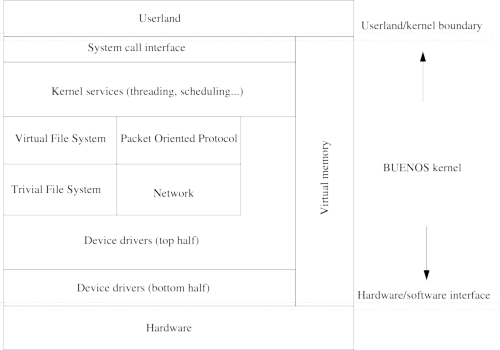
\includegraphics[width=\tablewidth,angle=0]{pics/architecture.png}
\caption{\kudos{} kernel overall architecture}
\label{fig:architecture}
\end{center}
\end{figure}

\index{hardware/software interface} \index{userland/kernel interface}
A simplified view of the \kudos{} kernel can be seen in
\autoref{fig:architecture}. At the top of the picture lies the
userland and at the bottom is the machine hardware. Neither of these
are part of the kernel, they just provide the context in which the
kernel operates. The userland/kernel boundary as well as the
hardware/software (hardware/kernel) interface are also marked in the
picture.

On the kernel side of these boundaries lies the important interface
code.  At the top, we can see the system call interface, which among
other userland related functionality is documented in
\autoref{sec:userland}. The system call interface is a set of
functions which can be called from userland programs\footnote{System
calls are important part of any OS. Try reading manual pages of
fork(2), wait(2), exec(2), read(2), write(2), open(2) and close(2) in
any Unix system for an example of the real thing.}. These functions
can then call almost any function inside the kernel to implement the
required functionality. Kernel functions cannot be called directly
from userland programs to protect kernel integrity and make sure that
the userland sandbox doesn't leak.

On the bottom boundary are the device drivers. Device drivers are
pieces of code which know how to use a particular piece of hardware.
Device drivers are usually divided into two parts: the top and bottom
halves. The bottom half of a device driver is an independent piece of
code which is run outside the kernel threading system whenever the
hardware generates an interrupt (this piece of code is called an
interrupt handler\index{interrupt!handler}). The top
half of the device driver is a set of functions which can be called
from within the kernel. The details of this, and description on how
the device driver halves communicate with each other are documented in
\autoref{sec:device}.

On top of the device drivers are various services which use device
drivers. Two examples can be seen in the picture: the filesystem and
the networking. The filesystem (see \autoref{sec:fs}) is actually
accessed through a module called the virtual filesystem (see
\autoref{sec:vfs}), which abstracts differences between different
filesystems. The filesystem itself uses a disk device driver to access
its permanent storage (the disk). Similarly the networking layer (see
\autoref{sec:network}), which uses network interface driver(s),
provides tools for sending and receiving network packets. The packet
oriented protocol module (POP, see \autoref{sec:pop}) uses the
networking module to provide socket and packet port (similar to UDP
ports in the Internet Protocol) functionality.

\subsection{Threading}

\index{threading, introduction}

Now we have seen an overview of various kernel services, but we still
don't have anything which can call these service functions. The core
of any kernel, including \buenos{}, is its threading and context
switching functionality. This functionality is sometimes called a
kernel by itself. Threading is provided by a threading library (see
\autoref{sec:threading}) in \buenos{}. The threading system makes it
possible to execute threads, separate instances of program
execution. Each thread runs independently of each other, alternating
their turns on the CPU(s). The context switching system is used to
switch one thread out of a CPU and to put a new one on it. Threads
themselves are unaware of these switches, unless they intentionally
force themselves out of execution (go to sleep).

Threads can be started by using the thread library. When starting a
thread it is given a function which it executes. When the function
ends, the thread dies. The thread can also commit suicide by
explicitly killing itself. Threads cannot kill each other, murders are
not allowed in the kernel (see exercises below). Each userland program
runs inside one thread. When the actual userland code is being run,
the thread cannot see the kernel memory, it can only access the system
call layer.

Threads can be pre-empted at any point, both in kernel and in
userland. Pre-empting means that the thread is taken out of execution
in favor of some other thread. The only way to prevent pre-empting is
to disable interrupts (which also disables timer interrupts used to
measure thread time-slices).

Since the kernel includes many data structures and many threads are
run simultaneously (we can have multiple CPUs), all data has to be
protected from other threads. The protection can be done with
exclusive access, achieved with various synchronization mechanisms
documented in \autoref{sec:sync}.

\subsection{Virtual Memory}

In the much referenced \autoref{fig:architecture}, there was one
more subsystem which hasn't been explained: the virtual memory (VM)
subsystem. As the figure implies, it affects the whole kernel,
interacts with hardware and also with the userland.

The VM subsystem is responsible for all memory handling operations in
the kernel. Its main function is to provide an illusion of private
memory spaces for userland processes, but its services are also used
in the kernel. Since memory can be accessed from any part of the
system, VM interacts directly with all system components.

\begin{figure}
\begin{center}
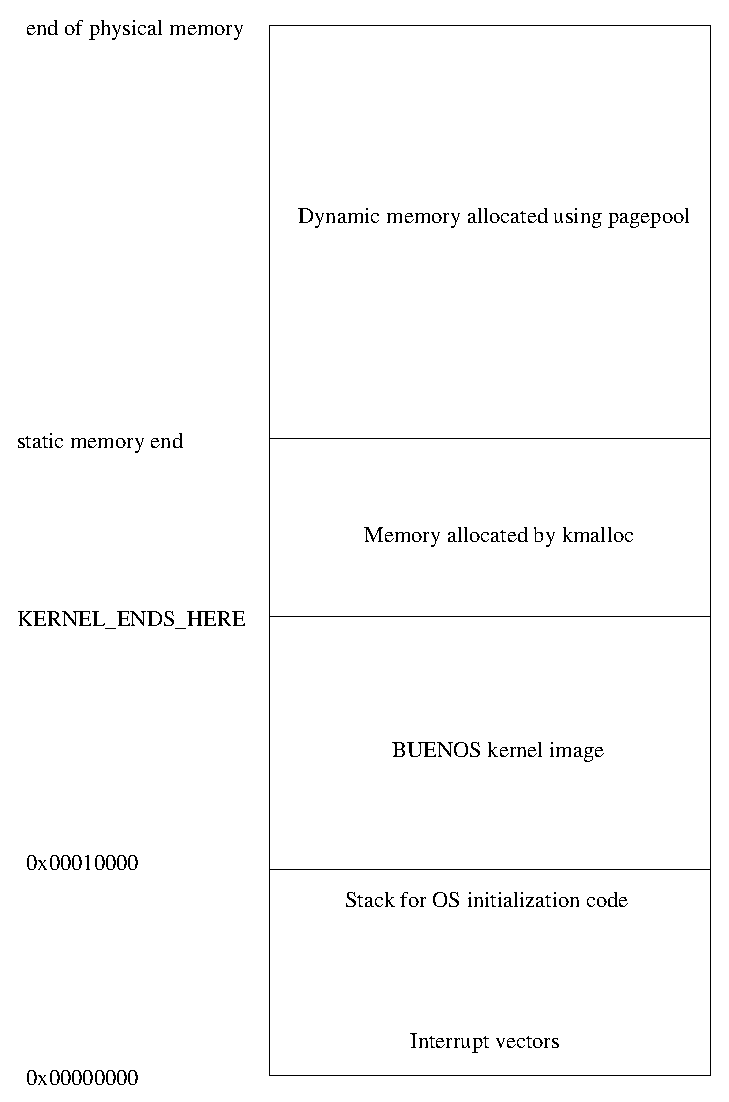
\includegraphics[width=\tablewidth,angle=0]{pics/buenos_memory.eps}
\caption{\buenos{} memory usage. Addresses are physical addresses.
Note that the picture is not in scale.}
\label{fig:buenosmemory}
\end{center}
\end{figure}

The physical memory usage in \buenos{} can be seen in
\autoref{fig:buenosmemory}. At the left side of the figure, memory
addresses can be seen. At the bottom is the beginning of the system
main memory (address zero) and at the top the end of the physical
memory.

The kernel uses part of this physical memory for its code (kernel
image), interrupt handling routines and data structures, including
thread stacks. The rest of the memory is at the mercy of the VM.

As in any modern hardware, memory pages (4096 byte regions in our
case) can be \emph{mapped} in \yams{}. The mapped addresses are also
called \emph{virtual addresses}. Mapping means that certain memory
addresses do not actually refer to physical memory. Instead, they are
references to a structure which \emph{maps} these addresses to the
actual addresses. This makes it possible to provide the illusion of
exclusive access to userland processes. Every userland process has
code at address \texttt{0x00001008}, for example. In reality this
address is in the mapped address range and thus the code is actually
on a private physical memory page for each process.

For more information on the virtual memory system and particularly on
the various address ranges, see \autoref{sec:vm}.

\subsection{Support for Multiple Processors}
\label{sec:SMP}
\index{SMP}

\buenos{} is a multiprocessor operating system, with pre-emptive
kernel threading. All kernel functions are thread-safe (re-entrant)
except for those that are used only during the bootup process.

Most code explicitly concerning SMP support is found in the bootstrap
code (see \autoref{sec:boot}). Unlike in real systems, where usually
only one processor starts at boot and it is up to it to start the
other processors, in \yams{} \emph{all} processors will start
executing code simultaneously and at the same address
(\texttt{0x80010000}). To handle this, the procedure described in
\autoref{sec:bootseq} is used.

Another place where the SMP support is directly evident is in the
context switch code, and in the code initializing data structures used
by the context switching code. Each processor must have its own stack
when handling interrupts, and each processor has its own current
thread. To account for these, the context switching code must know the
processor on which it runs.

Finally, a warning: implementing all virtual memory exercises on a
multiprocessor machine can be hard. It is suggested that for VM
exercises, only one CPU is used\footnote{The reasons become evident
when the inner details of the VM subsystem are covered later. For the
curious: the problem arises from the fact of having multiple TLBs, one
for each CPU. (The TLB is a piece of hardware used to map memory pages.)}.

Otherwise, the SMP support should be completely transparent. Of course
it means that synchronization issues must be handled more carefully,
but mostly everything works as it would on a single CPU system.

\section{Kernel Programming}

\index{kernel!programming}

Kernel programming differs somewhat from programming user
programs. This section explains these differences and also introduces
some conventions that have been used with \buenos{}.

\subsection{Memory Usage}

\index{memory!using in the kernel}
\index{kernel!using memory}

The most significant difference between kernel programming and
programming of user programs is memory usage. In the MIPS32
architecture, which \yams{} emulates, the memory is divided into
segments\index{segments, memory} \index{memory!segments}. Kernel code
can access all these segments while user programs can only access the
first segment called the \emph{user mapped segment}. In this segment
the first bit of the address is 0. If the first bit is 1, the address
belongs to one of the kernel segments and is not usable in
userland. The most important kernel segment in \buenos{} is the
\emph{kernel unmapped segment}, where addresses start with the bit
sequence 100. These addresses point to physical memory locations. In
kernel, most addresses are like this.  More information about the
memory segments can be found in \autoref{sec:segments}.

When initializing the system, a function (\texttt{kmalloc})
\index{kmalloc@\texttt{kmalloc}} is provided to allocate memory in
arbitrary-size chunks. This memory is permanently allocated and cannot
be freed. Before initializing the virtual memory system
\texttt{kmalloc} is used to allocate memory. After the initialization
of the virtual memory system \texttt{kmalloc} can no longer be used.
Instead, memory is allocated page by page from the virtual memory
system. These pages can be freed later.

\subsection{Stacks and Contexts}

\index{stack}
\index{interrupt!stack}
\index{kernel!stack}
\index{stack!kernel}

A stack is needed always when running code that is written in C. The
kernel provides a valid stack for user programs so the programmer does
not need to think about this. In kernel, however, nobody else provides
you with a valid stack. Every kernel thread must have its own stack.
In addition, every CPU must have an interrupt stack because thread
stacks cannot be easily used for interrupt processing. If a kernel
thread is associated with a user process, the user process must also
have its own stack. \buenos{} already sets up kernel stacks and
interrupt stacks appropriately.

Because the kernel and interrupt stacks are statically allocated,
their size is limited. This means that large structures and tables
cannot be allocated from stack. (The variables declared inside a
function are stack-allocated.) Note also that recursive functions
allocate space from the stack for each recursion level. Deeply
recursive functions should thus not be used.

\index{context}

Code can be run in several different contexts. A context consists of a
stack and CPU register values. In the kernel there are two different
contexts. Kernel threads are run in a normal kernel context with the
thread's stack. Interrupt handling code is run in an interrupt context
with the CPU's interrupt stack. These two contexts differ in a
fundamental way. In the kernel context the current context can be
saved and resumed later. Thus interrupts can be enabled and blocking
operations can be called. In the interrupt context this is not
possible so interrupts must be disabled and no blocking operations can
be called. In addition, if a kernel thread is associated with a
userland process, it must also have a userland context.

\subsection{Library Functions}

\buenos{} provides several library functions in the directory
\texttt{lib/}. These include functions for string processing and
random number generation. These functions are needed because standard
C library cannot be linked with \buenos{}. The prototypes of these
functions can be found in \texttt{lib/libc.h}.

\subsection{Using a Console}

\index{console}
\index{kprintf@\texttt{kprintf}}
\index{kwrite@\texttt{kwrite}}

In the kernel, reading from and writing to the console is done by
using the polling TTY driver. The \texttt{kprintf} and \texttt{kwrite}
functions can be used to print informational messages to the user.
Debug printing should be handled with the \texttt{DEBUG} function.
This way debug messages can be easily disabled later when
they are no longer needed. Userland console access should not be
handled with these functions. The interrupt driven TTY driver should
be used instead. See the example in \texttt{init/main.c}.

\subsection{Busy Waiting}

\index{busy waiting}

In the kernel, special attention has to be given to synchronization
issues.  Busy waiting must be avoided whenever possible. The only
place where busy waiting is acceptable is the spinlock
implementation, which is already done for you. Because spinlocks use
busy waiting, they should never be held for a long time.

\subsection{Floating Point Numbers}

\index{floating point numbers}
\index{co-processor unusable exception}

\yams{} does not support floating point numbers so they cannot be used
in \buenos{} either. If an attempt to execute a floating point
instruction is made, a co-processor unusable exception will occur.
(The floating point unit is co-processor 1 in MIPS32 architecture.)

\subsection{Naming Conventions}

\index{naming conventions}

Some special naming conventions have been used when programming
\buenos{}.  These might help you find a function or a variable when
you need it. Functions are generally named as
\texttt{filename\_function} where \texttt{filename} is the name of the
file where the function resides and \texttt{function} tells what the
function does. Variables are named similarly
\texttt{filename\_variable}.

\subsection{Debug Printing}

\index{debug printing}

Sometimes it is usefull to be able to print debugging information from
the kernel. A function which uses the polling TTY driver is provided
for such printing. Because polling TTY driver is used, printing is
possible from all parts of the kernel. Note that printing with the
polling driver slows the system down considerably and also changes
system timings which may cause trouble when debugging a SMP system.

\begin{function}{void}{DEBUG}{char *debuglevelname, char *format, ...}

\item If \texttt{debuglevelname} has been given to the kernel as a boot
argument, prints debug information. If not, ignores the debug printing.

\item \texttt{format} and other arguments are given as for \texttt{printf()}.

\end{function}


\subsection{C Calling Conventions}
\label{callingconvention}

\index{calling convention}
\index{C calling convention}

Normally C compiler handles function calling conventions (mostly
argument passing) transparently. Sometimes in kernel code the calling
convention issues need to be handled manually. Manual calling
convention handling is needed when calling C routines from a assembly
program or when manipulating thread contexts in order to pass
arguments to starting functions.

Arguments are passed to all functions in MIPS argument registers
\texttt{A0}, \texttt{A1}, \texttt{A2} and \texttt{A3}. When more than
4 arguments are needed, the rest are passed in the stack. The
arguments are put into the stack so that the 1st argument is in the
lowest memory address.

There is one thing to note: the stack frame for arguments must always
be reserved, even when all arguments are passed in the argument
registers. The frame must have space for all arguments. Arguments
which are passed in registers need not to be copied into this reserved
space.

\subsection{Kernel Boot Arguments}

\index{kernel!boot arguments}
\index{boot arguments}

\yams{} virtual machine provides a way to pass boot arguments from the
host operating system to the booted kernel. \buenos{} supports these
arguments. Please see \autoref{sec:bootargs} for details.


\begin{exercises}

\exercise{In \buenos{}, a thread that is ready to be run will be run
on whichever processor first removes it from the scheduler's ready
list. This can cause the thread to bounce from processor to processor on
every timeslice. This behavior is also present in real operating
systems, e.g. Solaris. Why might this behavior not be a good idea?}

\exercise{In \buenos{} threads cannot kill each other. There are many
reasons for this, try to figure out as many as you can.}

\end{exercises}


\chapter{Threading and Scheduling}
\label{sec:threading}

\index{threading system}

This chapter describes the threading system implemented in \buenos{}.
The kernel can run multiple threads and schedule them across any
number of CPUs the system happens to have. 

The threading system contains three major parts: thread library,
scheduler and context switching code. Each of these components is
thoroughly explained below in their own sections.

The thread library contains functions for thread creation, running and
finishing (dying). It also implements the system wide table of threads.

Scheduler handles the allocation of CPU time for runnable threads.

Context switch code is executed when an exception (trap or interrupt)
occurs. Its purpose is to save and restore execution contexts (CPU
register states, memory mappings etc.) of threads.

The context switching part is the most complicated and most hardware
dependent part of the threading system. It is not necessary to
understand it fully to be able to understand the whole threading
system. However, it is essential to see the purpose of all these three
parts.

For an introduction to these concepts, read either \cite{stallings} p.
108--123, 154--161, 394--407 and 438--449 or \cite{tanenbaum} p. 81--100
and 132--145.

\section{Threads}
\label{sec:threads}

\index{threads}
\index{thread\_table@\texttt{thread\_table}}

\buenos{} kernel supports multiple simultaneously running threads. One
thread can be run on each available CPU at a given moment. Information
on existing threads is stored in a fixed size table
\texttt{thread\_table}. The structure of the table is described in
detail in \autoref{sec:threadtable}.

Threads and thread table are handled through a collection of library
functions, that will do all necessary manipulation of the data
structures. They will also take care of concurrency. Thread handling
functions are described in \autoref{sec:threadlib}.

State diagram of \buenos{} threads is presented in
\autoref{fig:thread_states}. States in detail are described below:

\index{threads!states}

\begin{itemize}
\item FREE \index{FREE@\texttt{FREE}} indicates that this row in
  \texttt{thread\_table} is currently unused.

\item RUNNING \index{RUNNING@\texttt{RUNNING}} threads are currently
on CPU. In case of multiple CPUs, several threads may have this state.

\item READY \index{READY@\texttt{READY}} threads are on the
scheduler's ready list and can be switched to RUNNING state.
 
\item SLEEPING \index{SLEEPING@\texttt{SLEEPING}} threads are
\textbf{not on CPU} and are in sleep queue. Sleeping threads are
waiting for some resource to be freed. When access to the resource is
granted, the thread is waken up and switched to READY state.
 
\item NONREADY \index{NONREADY@\texttt{NONREADY}} threads have been
created, but are not yet marked to be runnable. The state is switched to
READY when the function \texttt{thread\_run()} is called.

\item DYING \index{DYING@\texttt{DYING}} threads have cleaned
themselves up, but are still on CPU. The scheduler should mark them FREE
when encountered.
\end{itemize}

\begin{figure}
\begin{center}
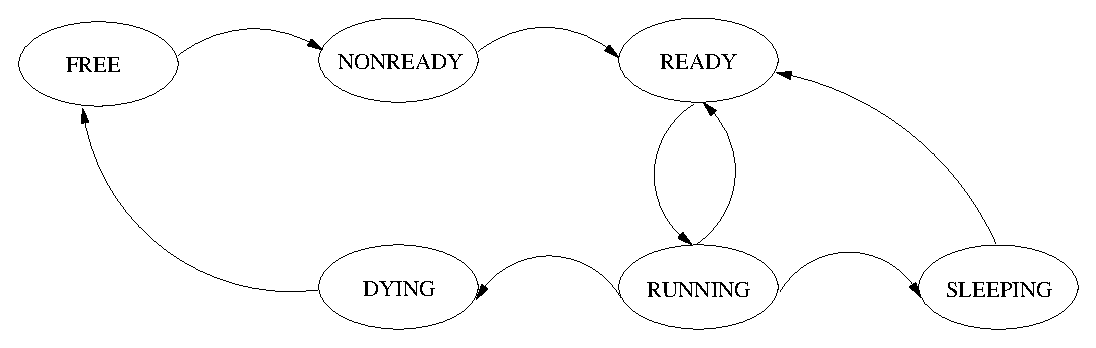
\includegraphics[width=\tablewidth]{pics/thread_states.ps}
\caption{\buenos{} thread states and possible transitions}
\label{fig:thread_states}
\end{center}
\end{figure}

\subsection{Thread Table}
\label{sec:threadtable}

\index{threads!table}

Thread table contains all necessary information about threads. This
information consists of:
\begin{itemize}
\item context of the thread, when it was running.
\item state of the thread. The state is used mostly by the scheduler,
when deciding which thread will be run next.
\item pagetable of the thread. Each thread will have its own virtual
memory mappings, so also own pagetables are needed.
\end{itemize}
All records and datatypes of thread table are described in
\autoref{tab:threadtable}.

\index{threads!ID}
\index{TID\_t@\texttt{TID\_t}}
\index{CONFIG\_MAX\_THREADS@\texttt{CONFIG\_MAX\_THREADS}}

Thread table is a fixed size (compile time option) structure, which
has one line for each thread. Threads are referenced by thread IDs
(\texttt{TID\_t}), which corresponds to index to the thread table. The
size of the table is defined in \texttt{kernel/config.h} by definition
\texttt{CONFIG\_MAX\_THREADS}. 

\index{thread\_table\_slock@\texttt{thread\_table\_slock}}

The thread table is protected by a single spinlock
(\texttt{thread\_table\_slock}). The lock must be a spinlock, because it
is used in contexts where threads cannot be switched for waiting (eg.
in scheduler). 

\index{thread\_table\_init@\texttt{thread\_table\_init}}

The thread table is initialized by calling
\texttt{thread\_table\_init()} function, which will set all thread
states to \texttt{FREE}.

\begin{table}
\begin{center}
\begin{tabularx}{\tablewidth}{l|l|>{\PBS\raggedright}X}
\textbf{Type}     & \textbf{Name}    & \textbf{Explanation} \\
\hline

context\_t * & context & Space for saving thread context. Context
consists of all CPU registers, including the program counter (PC) and
the stack pointer (SP). This pointer always refers to the thread's
stack area.\\

\hline

context\_t * & user\_context & Pointer to this thread's context in
userland. Field is NULL for kernel only threads. \\

\hline

thread\_state\_t & state & The current state of the thread. Valid
values are: \texttt{FREE}, \texttt{RUNNING}, \texttt{READY},
\texttt{SLEEPING}, \texttt{NONREADY} and \texttt{DYING}. \\

\hline

uint32\_t & sleeps\_on & If nonzero, tells which resource the
thread is sleeping on (waiting for). Nonzero value also indicates that
the thread is in some list in sleep queue. Note that the thread might
still be running and in middle of the process to go sleeping (in
which case its state is \texttt{RUNNING}.) \\

\hline

pagetable\_t * & pagetable & Pointer to the virtual memory mapping for
this thread. This entry is \texttt{NULL} if the thread does not have a
page table.\\

\hline

process\_id\_t & process\_id & Index to the process entry. This field
is currently unused, but thread creation sets this to a negative
value. \\

\hline

TID\_t & next & Pointer to next thread in this list. Used for forming
lists of threads (ready to run list, sleep queue). If this is the last
thread of a list, the value is negative. \\

\hline

uint32\_t & dummy\_alignment\_fill[9] & This is needed because
\texttt{thread\_table} entries are expected to be 64 bytes long (by
context\_switch code). If new fields are added or old ones are removed
this alignment should also be corrected in a proper way.

\end{tabularx}
\end{center}
\caption{Fields in thread table record}
\label{tab:threadtable}
\end{table}


\subsection{Thread Library}
\label{sec:threadlib}

\index{threads!library}

Thread library provides functions for thread handling.

\subsubsection{Thread Creation Functions}

\index{threads!creation}
\index{creating!a thread}

Threads can be manipulated by following functions implemented in
\texttt{kernel/thread.c}:

\begin{function}{TID\_t}{thread\_create}{void (*func)(uint32\_t), uint32\_t arg}

\item Creates a new thread by allocating a slot from
\texttt{thread\_table}. PC in this thread's context is set to the
beginning of the \texttt{func} and parameters are saved to the proper
registers in context. The context is saved in the stack area of the
newly created thread. When the scheduler decides to run this thread,
context is restored and it looks like function \texttt{func} would
have been called. The return address of the context is set to
beginning of the function \texttt{thread\_finish}.

\item Returns the thread ID of the created thread. If the return value
is negative, thread could not be created. The possible reasons for
failure are: full thread table and virtual memory shortage.

\item The argument \texttt{arg} is passed to the \texttt{func} which is
called when the new thread starts after a call to \texttt{thread\_run()}.

\end{function}


\begin{function}{void}{thread\_run}{TID\_t t}

\item Calls \texttt{scheduler\_add\_ready(t)}, which sets the thread
  state to \texttt{READY} and adds the thread to the ready-to-run list.

\end{function}

\subsubsection{Self Manipulation Functions}

The following functions can be used by a thread to manipulate itself:

\begin{function}{void}{thread\_switch}{void}

\item Perform voluntary context switch. Scheduler will later add the
thread to ready to run list if the thread is not sleeping on something
(\texttt{sleeps\_on} \index{sleeps\_on@\texttt{sleeps\_on}} is zero).
Context switch is performed by causing the software interrupt 0
\index{software interrupt 0} which is handled the same way as the
context switch. Interrupts are enabled before raising the software
interrupt, since otherwise the switch might not happen. The interrupt
state is restored before returning from this function.

\item Note that there is also a macro called \texttt{thread\_yield}
which points to this function. Since yielding is mechanically
equivalent to switching, the implementation is the same. The name
yielding is used when the yield has no actual effect, switching is
used when something actually happens (thread goes to sleep).

\end{function}

\begin{function}{void}{thread\_finish}{void}

\item Commit suicide. The thread calling this function will terminate
itself and free its resources (stack and thread table
entry). The thread marks its state to be \texttt{DYING}. The row in
thread table is later freed in the scheduler.

\item If a pagetable has been reserved for this thread it must be
freed before calling \texttt{thread\_finish}.

\end{function}


\begin{function}{TID\_t}{thread\_get\_current\_thread}{void}

\item Returns the TID \index{threads!ID} \index{TID@\texttt{TID}} of
the calling thread.

\end{function}


\begin{filelist}
\file{kernel/thread.c, kernel/thread.h}{Thread library}
\file{kernel/\_interrupt.s, kernel/interrupt.h}
{Interrupt mask setting functions}
\end{filelist}


\section{Scheduler}
\label{sec:scheduler}
\index{scheduler}

\index{threads!priority}
\index{priority, thread}

Scheduler is a piece of code that allocates CPU time for threads. The
basic \buenos{} scheduler is pre-emptive and allocates CPU time in a
round robin manner. Threads do not have priorities. Even threads
currently in kernel can be interrupted when their time slice has been
spent. This can be prevented by disabling interrupts.

\index{timeslice}
\index{CONFIG\_SCHEDULER\_TIMESLICE@\texttt{CONFIG\_SCHEDULER\_TIMESLICE}}

The timeslice allocated for a thread is defined in
\texttt{kernel/config.h} and the name of the configuration variable is
\texttt{CONFIG\_SCHEDULER\_TIMESLICE}. The value defines how many CPU
cycles a thread can use before it will be interrupted and next thread
will be selected for running. Timeslice includes the time spent in
context restoring, so it must be at least 250 cycles to guarantee that
the thread will get at least some real processing done. The actual
timeslice length is determined randomly and is at least the configured
number of ticks, see \autoref{sec:bootargs}.

\index{scheduler\_current\_thread@\texttt{scheduler\_current\_thread}}
\index{scheduler\_ready\_to\_run@\texttt{scheduler\_ready\_to\_run}}
Scheduler works by maintaining a global
\texttt{scheduler\_current\_thread} table of current threads (one per
CPU). It also has a list of ready threads, maintained in the local list
variable \texttt{scheduler\_ready\_to\_run}. The actual implementation
of the ready list is two indexes. One points to the beginning of the list in
thread table and the other to the end. A negative value in both head and
tail indicates an empty list.

\index{scheduler!locking}
\index{thread\_table\_slock@\texttt{thread\_table\_slock}}
The whole scheduler is locked by one spinlock to prevent multiple CPUs
entering the scheduler at the same time. Interrupts are always disabled
when scheduler is running, because it is called only from interrupt
and exception handlers. The spinlock used is
\texttt{thread\_table\_slock} and it also controls the access to the
thread table.

\index{timeticks}\index{timeslice}
\index{timer!interrupt}
Time ticks are handled by the CPU co-processor 0 counter mechanism. A timer
interrupt is generated when the counter meets the compare value (time slice
is over). The master interrupt handler will call the scheduler when a timer
interrupt has occured. Scheduler will also be called if software
interrupt 0 occured (thread gave up its timeslice) or when any
interrupt occurs and idle thread is currently running on the current CPU.
A new timer interrupt is scheduled after the scheduler has selected a new
running thread.

\index{ready to run list}
\index{DYING@\texttt{DYING}}
\index{RUNNING@\texttt{RUNNING}}
\index{FREE@\texttt{FREE}}
\index{SLEEPING@\texttt{SLEEPING}}
\index{READY@\texttt{READY}}
When the scheduler is entered, the current thread is checked. If the
current thread's state is marked as \texttt{DYING} or \texttt{RUNNING}
and sleeping on something (\texttt{sleeps\_on}
\index{sleeps\_on@\texttt{sleeps\_on}} is nonzero, see
\autoref{sec:sleepq}) the current thread is not placed on the
ready-to-run list, but its state is updated. For \texttt{DYING}
threads the state is changed to \texttt{FREE} and for \texttt{RUNNING}
(and sleeping) threads to \texttt{SLEEPING}. In all other cases the
thread is placed at the end of the ready-to-run list and its state is
updated to \texttt{READY}.

\begin{function}{void}{scheduler\_schedule}{void}
\item Selects the next thread to run. Updates
\texttt{scheduler\_current\_thread}
\index{scheduler\_current\_thread@\texttt{scheduler\_current\_thread}}
for current CPU. This \textbf{must not} be called from any thread,
only from the interrupt handler.

\item Implementation:
\begin{enumerate}

\item Lock the thread table by \texttt{thread\_table\_slock}
\index{thread\_table\_slock@\texttt{thread\_table\_slock}} spinlock
(interrupts \textbf{must} be off when calling this function, so they
are not explicitly disabled).

\item If the current thread state is \texttt{DYING}, mark it
\texttt{FREE}. This releases the thread table entry for reuse.

\item Else, if the thread is sleeping on something, just mark the
state as \emph{Sleeping}. The thread has placed itself on sleep queue
before explicitly switching to scheduler.

\item Else, add the current thread to the end of
\texttt{scheduler\_ready\_to\_run}
\index{scheduler\_ready\_to\_run@\texttt{scheduler\_ready\_to\_run}}
and mark it \texttt{READY}. Idle thread \index{idle thread} (thread 0)
is never added to this list.

\item Remove the first thread from \texttt{scheduler\_ready\_to\_run}.
This might be the same thread placed on the list in the previous step.
The function that will return the removed thread will return 0 (idle
thread) if the ready to run list was empty.

\item Mark the removed thread as \texttt{RUNNING}.

\item Release the thread table spinlock.

\item Set the removed thread as the current thread for this CPU.

\item Set the hardware timer to generate an interrupt after configured
number of ticks.

\end{enumerate}
\end{function}

Threads can be added to the scheduler's ready list by calling the
following function. This function is called \emph{only} from the
thread library function \texttt{thread\_run}
\index{thread\_run@\texttt{thread\_run}} and from the synchronization
library.

\begin{function}{void}{scheduler\_add\_ready}{TID\_t t}
\item Adds the thread \texttt{t} to the end of the ready-to-run list.
\item Implementation:
\begin{enumerate}
\item Lock the thread table (interrupts off, take thread table spinlock).
\item Add \texttt{t} to the end of the list
\texttt{scheduler\_ready\_to\_run}.
\item Release the thread table spinlock, restore interrupt status.
\end{enumerate}
\end{function}

\subsection{Idle thread}
\index{idle thread}
\index{IDLE\_THREAD\_TID@\texttt{IDLE\_THREAD\_TID}}

The idle thread, TID 0 (or \texttt{IDLE\_THREAD\_TID}), is a special
case of a thread. Its context is not saved (and \emph{must not}
be saved on a SMP machine) and it can be running simultaneously on
many CPUs. When restoring its context, only PC needs to be restored.
The idle thread will enter a neverending waiting loop whenever run.
Note that since the thread is used simultaneously on all CPUs, the code
cannot do anything useful!

\begin{filelist}
\file{kernel/scheduler.c, kernel/scheduler.h}{Scheduler}
\end{filelist}


\section{Context Switch}
\index{context switch!definition}

Context switching is traditionally the most bizarre piece of code in
most operating system implementations. There are many reasons for
this. One of them is that the context switch code must be written in
assembler and not in any high level language. Another reason is the
fact that it might be hard to follow the execution when the context of
execution changes. Unfortunately context switching is also the hardest
to understand of all parts of \buenos{}. Luckily, it is not necessary
to fully comprehend it to be able to understand the whole system.

\index{context}
Before going into details we must define what is actually meant by a
context or context switching. In the scope of the threading system, a
context means some particular computation process (note that this is
not the same thing as userland process). This piece of code is mostly
unaware that any other code is being run on the same CPU. It is the
responsibility of the threading system to provide an illusion for
other pieces of code that they run in an isolated environment.

\index{exception}
\index{timer!interrupt}
\index{interrupt!handler}
Thus when the need arises to give CPU time to some other part of the
system the currently running code (thread) is interrupted. This might
happen for three distinct reasons. An exception might have occured in
kernel mode and the cause of the exception needs to be examined. An
exception can also have occured in user mode in which case the thread
wishes to switch from its user context to kernel context. An interrupt
might have occured and CPU time needs to be given to the interrupt
handler. This case covers also the special case of a timer interrupt.
The timer interrupt is served in an interrupt handler and after the
handler returns a new piece of code (thread) is running and the old is
waiting for its turn to get the CPU. To be able to do all this
transparently, the system needs to save state information on the
interrupted thread. This state information is the context of that
thread and in \buenos{} this information is saved in the kernel stack
area of the thread.

\index{program counter}
\index{stack pointer}
The exact details of the contents of thread contexts are described
later, but the most important part of the data is the contents of the
CPU registers. The values of the registers are saved and those of the
new thread are put into the CPU registers. Since the registers contain
the program counter and the stack pointer, both threads can be unaware of
each other. The process of saving the state of one thread and
restoring the state of some other thread is called context switching.

\index{execution context}
\index{interrupt!handler}
It should be noted that threads are not the only entities having
execution contexts. Interrupt handler(s) needs to have its own private
context which can be used at any time when an interrupt occurs. All
context switching and interrupt handling are done in the context of
interrupt handling, by using a separate stack area reserved for
serving interrupts. The high level interrupt handlers are described in
detail in \autoref{sec:inthandlers}.

\subsection{Interrupt Vectors}
\index{interrupt!vectors}
\index{kernel\_interrupt\_stacks@\texttt{kernel\_interrupt\_stacks}}

First thing to do in order to have proper interrupt/exception handling
is to set up the MIPS interrupt/exception handler vectors. This is
done during the boot up. Also, in boot, interrupt handler stack
\texttt{kernel\_interrupt\_stacks} must be allocated for each CPU
present in the \yams{} simulator.

\index{blocking interrupts}
A few words on the difference of interrupts and exceptions; interrupt
is a coordinated interruption of execution caused by raise of either
hardware or software interrupt line. Interrupts can be blocked by
setting an appropriate interrupt mask. Exceptions and traps are caused by
CPU instructions either on purpose (traps to syscalls), as a side
effect (TLB miss) or by accident (divide by zero). Exceptions cannot
be blocked.

All interrupts and exceptions transfer control to three special
Interrupt Vector Areas. These areas are located in memory addresses
0x80000000, 0x80000180 and 0x80000200. The maximum size of these areas is
32 bytes, so each of them can fit only 8 instructions.

\index{cswitch\_switch@\texttt{cswitch\_switch}}
\index{cswitch\_vector\_code@\texttt{cswitch\_vector\_code}}
It is obvious that the real interrupt handling code cannot be written
to area of size of 8 instructions. Therefore, these interrupt vector
areas contain only a jump to an assembler routine labeled
\texttt{cswitch\_switch} and a delay slot instruction. This code is
labeled as \texttt{cswitch\_vector\_code}. The label is needed so that
the code can be injected into the interrupt handler vector area. The
size of this code is 8 words (instructions) or 32 bytes\footnote{The
size of interrupt vector area is mandated by the location of the next
interrupt vector. The vector size is cleverly chosen by hardware
designers to be long enough to contain TLB refilling code. We avoid
that (good, efficient and realistic) solution to make it possible to
handle TLB misses in C.}.

The assembly code in the interrupt vector is just a jump to
\texttt{\_cswitch\_switch}-function.

\index{interrupt\_init@\texttt{interrupt\_init}}
Now, the problem is, how to inject the above assembly code to its
proper place in the interrupt handler vector. This is done by finding
the interrupt handler code address from label
\texttt{cswitch\_vector\_code} and copying two words from there to the
memory areas 0x80000000, 0x80000180 and 0x80000200. This code is
written in C and is a part of \texttt{interrupt\_init()} function in
\texttt{kernel/interrupt.c}.

\subsection{Context Switching Code}
\index{context switch!implementation}

\index{\_cswitch\_switch@\texttt{\_cswitch\_switch}}
Actual context switch related functions are performed in the
\texttt{\_cswitch\_switch} code. This code is written in assembly
language because the interrupt handler stack is not yet usable and
therefore we cannot use C-functions. We also must be careful that we
don't use any registers which are not saved.

The general processing of a context switch is the same for all three
causes (kernel mode exception, user mode exception and interrupt) for
entering the context switch code. It consists of the following actions
(in this order):

\begin{description}
\item[Save current context.] \index{context!saving} Data is saved from
  processor to the \texttt{context\_t}
  \index{context\_t@\texttt{context\_t}} data structure in the kernel
  stack area of the currently running thread. The structure of the
  current thread is pointed by global variable
  \texttt{scheduler\_current\_thread}
  \index{scheduler\_current\_thread@\texttt{scheduler\_current\_thread}}
  (see \autoref{sec:scheduler}). The current thread is found from
  \texttt{scheduler\_current\_thread}-table, indexed by CPU number.
  The following things are saved:
  \begin{itemize}
  \item Co-processor 0 EPC register contains Program Counter value
    before jump to interrupt handler.
  \item All CPU registers including hi and lo except k0 and k1.
  \item Status register (Co-processor 0) fields UM (bit 4), IM0--IM7
  (bits 8--15), IE (bit 0). This saves the interrupt mask of the
  current thread and remembers whether we came from userland (UM bit
  enabled) or from kernel (UM bit is zero).
  \item Link to the \texttt{context\_t} saved to the thread structure.
  Thus when nested exceptions or interrupts occur, we can unfold this
  list one reference per context switch and finally come back to the
  actual running context of the thread.
  \end{itemize}

\item[Initialize stack.] A stack is needed to be able to call C
  functions. If we are going to handle interrupts and/or reschedule
  threads, we set up stack in the interrupt stack area. In other cases
  we use thread's kernel stack.

\item[Call the appropriate function to handle the exception/interrupt]
  This is a C function which will take care of the interrupt/exception
  processing.

\item[Restore new context.] \index{context!restoring} After the
interrupt/exception is handled, context is restored from
\texttt{scheduler\_current\_thread}. Note that in
\texttt{interrupt\_handle}
\index{interrupt\_handle@\texttt{interrupt\_handle}} the scheduler
might have changed the currently running thread to something else than
the one we just saved. Therefore we might start running a new thread at
this point.

\item[Return with ERET] PC is restored from EPC by this special machine
instruction. The EXL bit preventing interrupts is also cleared by the
CPU.

\end{description}

\index{interrupt!stack area} \index{stack!for interrupts}
\index{interrupt\_handle@\texttt{interrupt\_handle}} 
\index{kernel\_interrupt\_stacks@\texttt{kernel\_interrupt\_stacks}}
\index{context}

In the case of an interrupt, the stack that is initialized is the
interrupt context stack. Interrupt stack pointers are defined in the table
\texttt{kernel\_interrupt\_stacks}. Table is indexed by CPU number.
The stack pointer is set to point to the interrupt stack reserved for
this CPU. Since we don't have nested interrupts, only one stack area
per CPU is sufficient. Then the function \texttt{interrupt\_handle} is
called. This C-function will call all registered interrupt handlers
and the scheduler, when appropriate. The function is implemented in
\texttt{kernel/interrupt.c}. Last the context is restored from current
thread's \texttt{context}. 

\index{interrupt!stack}
We use interrupt stacks also for scheduler running, because we cannot
continue to run in a stack of some other thread after the context has
been switched. If we used the kernel stacks of threads, some other CPU
might have picked up our previous thread and run it and thus mess up
our stack.

\index{exception!handling}
\index{kernel\_exception\_handle@\texttt{kernel\_exception\_handle}}

If an exception has occured in kernel mode, it is handled mostly the
same way as an interrupt except that instead of calling the function
\texttt{interrupt\_handle}, the function
\texttt{kernel\_exception\_handle} is called. The only other difference is
that we use the kernel stack area of the current thread instead of the
interrupt stack area. The handling function is implemented in
\texttt{kernel/exception.c}.

\index{exception handling}
\index{user\_exception\_handle@\texttt{user\_exception\_handle}}

When an exception occurs in user mode, the thread wishes to switch
from its user context to kernel context. The stack is initialized to
the current position of the kernel stack of this thread. The stack
information is dug from previous context information, usually from
the initial context of the thread. 

Because the thread is switching from user mode to kernel mode the base
processing mode of the processor (indicated by the UM bit \index{UM
bit} in Status register) is changed to kernel mode. The user mode
exceptions are handled by the function
\texttt{user\_exception\_handle}, which is implemented in
\texttt{proc/exception.c}. This function will enable interrupts by
setting the EXL bit \index{EXL bit} in the Status register and handle
the user mode exception. After returning from this function the
context is restored normally from saved context information.

\index{cswitch\_switch@\texttt{cswitch\_switch}}

The basic structure of the \texttt{cswitch\_switch} is thus the
following\footnote{We need to disable GNU Assembler instruction
reordering and macro instruction usage because their interpretation
needs some special registers that are not yet saved.}:

\begin{verbatim}
     .set noreorder
     .set nomacro

cswitch_switch:
     <figure out the appropriate context_t structure>
     j cswitch_context_save
     nop
     <init stack>      # After this we can call C-functions
     <change base mode if appropriate>
     <set up arguments to *_hanlde>
     <call *_handle>
     <figure out the appropriate context_t structure>
     j cswitch_context_restore
     nop
     eret

     .set reorder
     .set macro
\end{verbatim}

Note that before the context is saved, we can only use the registers
k0 and k1, which are reserved for the kernel by MIPS calling
convention.

\subsection{Thread Contexts}
\label{sec:threadcontext}
\index{context\_t@\texttt{context\_t}}
\index{thread\_t@\texttt{thread\_t}}
\index{threads!context}
\index{context!saving area}
\index{threads!table}

The context of a thread is saved in the \texttt{context\_t} structure,
which is usually referenced by a pointer in \texttt{thread\_t} in
thread table (see \autoref{sec:threadtable}). Contexts are always
stored in the stack of the corresponding thread. It has the following
fields:

\begin{center}
\begin{tabularx}{\tablewidth}{l|l|>{\PBS\raggedright}X}
\textbf{Type}     & \textbf{Name}    & \textbf{Explanation} \\
\hline

uint32\_t[29] & cpu\_regs & CPU registers except zero, k0 and k1. That
makes 29 registers. \\
\hline

uint32\_t & hi & The hi register. \\
\hline

uint32\_t & lo & The lo register. \\
\hline

uint32\_t & pc & PC register which can be obtained from the CP0
register EPC. \\
\hline

uint32\_t & status & The saved bits of the CP0 status register. \\
\hline

void * & prev\_context & Link to previous saved context. This field
links saved contexts up to the point when the thread was initially
started. \\

\end{tabularx}
\end{center}

\begin{filelist}
\file{kernel/cswitch.S}{\texttt{\_cswitch\_vector\_code},
                        \texttt{\_cswitch\_switch},
                        \texttt{\_cswitch\_context\_save},
                        \texttt{\_cswitch\_context\_restore}}
\file{kernel/interrupt.c}{\texttt{interrupt\_handle}}
\file{kernel/cswitch.h}{\texttt{context\_t}}
\end{filelist}

%% XXX Where does this section really belong???
\section{Exception Processing in Kernel Mode}

\index{kernel!exceptions}
\index{exception!kernel exceptions}

When an exception occurs in kernel mode, the function
\texttt{kernel\_exception\_handle} is called. The cause of an
exception in kernel might be a TLB miss or there might be a bug in the
kernel code.

\begin{function}{void}{kernel\_exception\_handle}{int exception}
\item This function is called when an exception has occured in kernel
  mode. Handles the given \texttt{exception}.
\item If kernel uses mapped addresses, this function should handle TLB
exceptions. Other exceptions indicate that there is some kind of bug in
the kernel code.
\item Implementation:
\begin{enumerate}
\item Panic with a message telling which exception has occured.
\end{enumerate}
\end{function}

\begin{filelist}
\file{kernel/exception.h, kernel/exception.c}
{\texttt{kernel\_exception\_handle}}
\end{filelist}

\begin{exercises}

\exercise{The context switching code is written wholly in assembler.
Why can it not be implemented in C? The code uses CPU registers
\texttt{k0} and \texttt{k1}, but it doesn't touch other registers
before the thread context has been saved. Why \texttt{k0} and \texttt{k1}
can be used in the code?}

\exercise{The current exception system in \buenos{} doesn't allow
interrupts to occur when an interrupt handler is running. What
modifications to the system are needed to implement a hierarchical
interrupt scheme where higher priority interrupts can occur while
lower priority ones are being served?}

\cexercise{The current \buenos{} scheduler doesn't have any priority
handling for threads. Implement a priority scheduler in which all
threads can be given a priority value. Higher priority threads will
get more processor time than lower priority threads. Your solution
should guarantee that no thread will starve (get no processor time at
all).}

\exercise{After you have implemented your priority scheduler, you
might have noticed an effect known as \emph{Priority inversion}. This
effect is caused by a situation where a high priority thread will
block and wait for a resource currently held by a low priority thread.
Since there might also be other threads in the system which have
higher priority than the thread holding the resource, it may not get
any CPU time. Therefore also the high priority thread is hindered as
if it had a low priority. How can this problem be prevented?}



\end{exercises}


\chapter{Synchronization Mechanisms}
\label{sec:sync}
\index{synchronization}

The \buenos{} kernel has many synchronization primitives which can be
used to protect data integrity. These mechanisms are interrupt
disabling, spinlocks, the sleep queue and semaphores. Locks and
condition variables are left as an exercise.

For an introduction on synchronization concepts, read either
\cite{tanenbaum} p. 100--132 and 159--164 or \cite{stallings} p. 198--253
and 266--274.

\section{Spinlocks}
\label{sec:spinlock}
\index{spinlock}

A spinlock is the most basic, low-level synchronization primitive for
multiprocessor systems. For a uniprocessor system, it is sufficient to
disable interrupts to achieve low-level sychronization (a
nonpre-emptible code region). When there are multiple processors, this
is obviously not enough, since the other processors may still
interfere. To achieve low-level interprocessor synchronization,
interrupts must be disabled \emph{and} a spinlock must be acquired.

Spinlock acquisition process is very simple: it will repeatedly check
the lock value until it is free (``spin''), then set the value to
taken. This will of course completely tie up the processor (since
interrupts are disabled), so code regions protected by a spinlock
should be as short as possible.

Disabling interrupts and spinlock acquiring can (and must) be used in
interrupt handlers since they must never cause a sleeping block.

In \buenos{}, the spinlock data type is a signed integer containing
the value of the lock.  Zero indicates that the lock is currently
free. Positive values mean that the lock is reserved. The exact value
can be anything, as long as it is positive. The value must never be
negative (reserved for future extensions).

Due to the nature of the spinlock implementation, spinlocks should
never be moved around in memory. In practice this means that they must
reside on the kernel unmapped segment which is not part of the virtual
memory page pool. This should not be a problem, since spinlocks are
purely a kernel synchronization primitive.

\subsection{LL and SC Instructions}

\index{LL instruction}
\index{SC instruction}
\index{test-and-set}
\index{RMW sequence}

To achieve safe synchronization for spinlock implementation in a
multiprocessor system, a version of a \emph{test-and-set} machine
instruction is needed. On a MIPS architecture, this is the LL/SC
instruction pair. The LL (load linked word) instruction loads a word
from the specified memory address. This marks the beginning of a RMW
(read-modify-write) sequence for that processor. The RMW sequence is
``broken'' if a memory write to the LL address is performed \emph{by
any processor}. If the RMW sequence was not broken, the SC (store
conditional word) instruction will store a register value to the
address given to it (the LL address) and set the register to 1. If the
RMW sequence was broken, SC will not write to memory and sets the
register to 0.

\subsection{Spinlock Implementation}

The following functions are available to utilize spinlocks. Note that
\emph{interrupts must always be disabled when a spinlock is held},
otherwise Bad Things will happen (see exercises below).

\begin{function}{void}{spinlock\_acquire}{spinlock\_t *slock}
\item Acquire given spinlock. While waiting for lock to be free, spin.
\begin{enumerate}
\item \texttt{LL} the address \texttt{slock}.
\item Test if the value is zero. If not, jump to case 1.
\item \texttt{SC} the address to one. If fails, jump to case 1.
\end{enumerate}
\end{function}

\begin{function}{void}{spinlock\_release}{spinlock\_t *slock}
\item Free the given spinlock.
\begin{enumerate}
\item Write zero to the address \texttt{slock}.
\end{enumerate}
\end{function}

\begin{function}{void}{spinlock\_reset}{spinlock\_t *slock}
\item Initializes the given spinlock to be free.
\item Implementation:
\begin{enumerate}
\item Set spinlock value to zero. This is actually an alias to
\texttt{spinlock\_release}.
\end{enumerate}
\end{function}


\section{Sleep Queue}
\label{sec:sleepq}
\index{sleep queue}
\index{resource waiting}
\index{waiting for a resource}

Thread level synchronization in kernel requires some way for threads
to sleep and wait for a resource, like a semaphore, to be available.
To avoid the need to implement the sleeping mechanism separately for
each such resource, a general sleeping mechanism called sleep queue is
implemented in \buenos{}.

\subsection{Using the Sleep Queue}
\index{sleep queue!usage}
\index{sleeping}
\index{using the sleep queue}

The sleep queue enables a thread to wait for a specific resource and
to be later woken up by some other thread which has released the
resource. The resource, on which the thread is sleeping, is identified
by an address. This address must be from the kernel unmapped segment
so that the different threads agree on it.

There are three functions which threads can call to manipulate the
sleep queue structure. The function \texttt{sleepq\_add}
\index{sleepq\_add@\texttt{sleepq\_add}} is called by a thread that
wishes to wait for a resource. The functions \texttt{sleepq\_wake}
\index{sleepq\_wake@\texttt{sleepq\_wake}} and
\texttt{sleepq\_wake\_all}
\index{sleepq\_wake\_all@\texttt{sleepq\_wake\_all}} are called by a
thread that wishes to wake up another thread. When using these
functions, careful thought has to be given to the synchronization
issues involved. The resource on which threads wish to sleep is
usually protected by a spinlock. Before calling the sleep queue
functions interrupts must be disabled and the resource spinlock must
be acquired. This ensures that the thread wishing to go to sleep will
indeed be in the sleep queue before another thread attempts to wake it
up.

If the resource spinlock is not held while calling the sleep queue
functions, the following scenario can happen. One thread concludes
that it wishes to go to sleep and calls \texttt{sleepq\_add}. Before
this call is serviced, another thread ends its business with the
resource and calls \texttt{sleepq\_wake}. No threads are found in the
sleep queue so no thread is woken up. Now the call to
\texttt{sleepq\_add} by the first thread is serviced and the first
thread goes to sleep. Thus in the end the resource is free, but the
first thread is still waiting for it.

The function \texttt{sleepq\_add} does not cause the thread to
actually go to sleep. It merely inserts the thread into the sleep
queue. The thread needs to call \texttt{thread\_switch}
\index{thread\_switch@\texttt{thread\_switch}} to release the CPU. The
scheduler will then notice that the thread is waiting for something
and change the state of the thread to \texttt{SLEEPING}. This mechanism
is needed because the thread needs to release the resource spinlock
before actually going to sleep. Because the thread calling
\texttt{sleepq\_add} holds a spinlock, it has also disabled
interrupts. Interrupts also need to be disabled to make sure that the
thread is not switch out and put to sleep before it is ready to do so.
Thus the \texttt{sleepq\_add} function checks that interrupts are
disabled.

The following is an example of the correct usage of the sleep queue.
The thread wishing to go to sleep executes the code shown in the
\autoref{fig:sleepqadd}. Lines 1 and 2 ensure protection from other
threads using this same resource. The while-loop on line 3 is
necessary if it is possible that some other thread can also get the
resource. Because we need to release the resource spinlock in the
while loop body, another thread might acquire the resource first. The
resource spinlock is released on line 5 because the thread cannot hold
it while it is not on CPU. Line 6 will make the scheduler choose
another thread to run.

\begin{figure}
\begin{center}
\begin{verbatim}
1  Disable interrupts
2  Acquire the resource spinlock
3  While we want to sleep:
4    sleepq_add(resource)
5    Release the resource spinlock
6    thread_switch()
7    Acquire the resource spinlock
8  EndWhile
9  Do your duty with the resource
10 Release the resource spinlock
11 Restore the interrupt mask
\end{verbatim}
\caption{Code executed by a thread wishing to go to sleep.}
\label{fig:sleepqadd}
\end{center}
\end{figure}

The thread, or interrupt handler, wishing to wake up a thread
executes the code shown in the \autoref{fig:sleepqwake}.

\begin{figure}
\begin{center}
\begin{verbatim}
1  Disable interrupts
2  Acquire the resource spinlock
3  Do your duty with the resource
4  If wishing to wake up something
5    sleepq_wake(resource) or sleepq_wake_all(resource)
6  EndIf
7  Release the resource spinlock
8  Restore the interrupt mask
\end{verbatim}
\caption{Code executed by a thread wishing to wake up another thread.}
\label{fig:sleepqwake}
\end{center}
\end{figure}

\subsection{How the Sleep Queue is Implemented}
\index{sleep queue!implementation}

Sleep queue is a structure which contains linked lists of threads
waiting for a specific resource. The actual structure is implemented
as a static size hashtable \texttt{sleepq\_hashtable}
\index{sleepq\_hashtable@\texttt{sleepq\_hashtable}} with separate
chaining. The chains are implemented using the
\texttt{thread\_table\_t}'s \texttt{next} field, which is also used
for the linked lists (all lists with same hash value are linked in the
same list, see the \autoref{fig:sleepq}). New threads are always added
to the end of the list and threads are released from the beginning of
the chain. This makes the wakeup operation run in shorter time and it
is desirable to have it this way, because it is often run in device
driver code. Also the first thread in the chain is not necessary the
thread we want to wake up.

\begin{figure}
\begin{center}
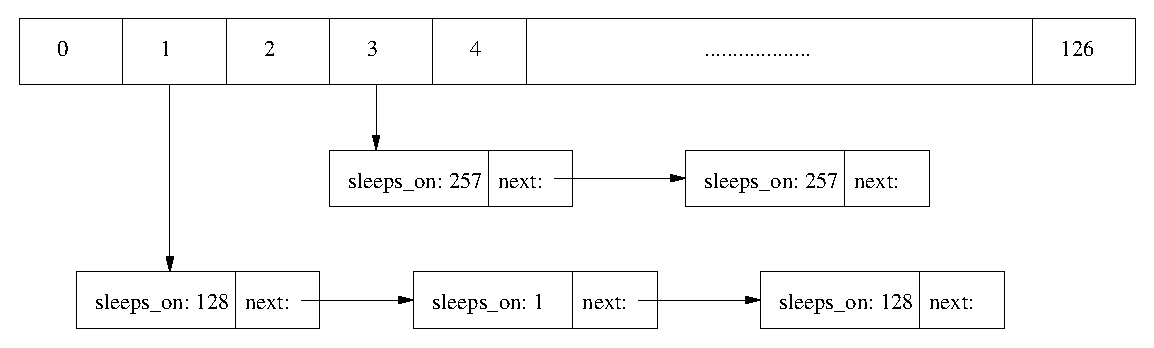
\includegraphics[width=\tablewidth,angle=0]{pics/sleepq.eps}
\caption{Linked lists in sleep queue.}
\label{fig:sleepq}
\end{center}
\end{figure}


To protect the hashtable from concurrent access, it is protected by a
spinlock \texttt{sleepq\_slock}
\index{sleepq\_slock@\texttt{sleepq\_slock}}. This lock must be held
and interrupts must be disabled in all sleep queue operations.

Threads are referenced in the sleep queue system by the resource they
are waiting for (sleeping on). The information is stored in
\texttt{thread\_table\_t} structure's field \texttt{sleeps\_on}
\index{sleeps\_on@\texttt{sleeps\_on}}. Zero in this field indicates
that the thread is not waiting for anything. The resource waiting is
in practice done by waiting for the address of a resource (a semaphore
struct, for example).

Sleep queue functions:

\begin{function}{void}{sleepq\_add}{void *resource}
\item Adds the currently running thread into the sleep queue. The
  thread is added to the sleep queue hashtable. The thread does not go
  to sleep when calling this function. An explicit call to
  \texttt{thread\_switch} is needed. The thread will sleep on the
  given \texttt{resource}, which is identified by its address.
\item Implementation:
\begin{enumerate}
\item Assert that interrupts are disabled. Interrupts need to be disabled
  because the thread holds a spinlock and because otherwise the thread
  can be put to sleep by the scheduler before it is actually ready to
  do so.
\item Set the current thread's \texttt{sleeps\_on} field to the
\texttt{resource}.
\item Lock the sleep queue structure.
\item Add the thread to the queue's end by hashing the address of
given resource.
\item Unlock the sleep queue structure.
\end{enumerate}
\end{function}

\begin{function}{void}{sleepq\_wake}{void *resource}
\item Wakes the first thread waiting for the given \texttt{resource}
from the queue. If no threads are waiting for the given
\texttt{resource}, do nothing.
\item Implementation:
\begin{enumerate}
\item Disable interrupts.
\item Lock the sleep queue structure.
\item Find the first thread waiting for the given resource by hashing the
resource address and walking through the chain.
\item Remove the found thread from the sleep queue hashtable.
\item Lock the thread table.
\item Set \texttt{sleeps\_on} \index{sleeps\_on@\texttt{sleeps\_on}}
to zero on the found thread.
\item If the thread is sleeping, add it to the scheduler's ready list
by calling \texttt{scheduler\_add\_to\_ready\_list}.
\item Unlock the thread table.
\item Unlock the sleep queue structure.
\item Restore the interrupt mask.
\end{enumerate}
\end{function}

\begin{function}{void}{sleepq\_wake\_all}{void *resource}

\item Exactly like \texttt{sleepq\_wake}, but wakes up all threads which
  are waiting for the given \texttt{resource}.
\end{function}

The sleep queue system is initialized in the boot sequence by calling the
following function:

\begin{function}{void}{sleepq\_init}{void}
\item Sets all hashtable values to -1 (free).
\end{function}


\begin{filelist}

\file{kernel/sleepq.h, kernel/sleepq.c}{Sleep queue operations}

\end{filelist}


\section{Semaphores}
\label{sec:semaphores}
\index{semaphores}

Interrupt disabling, spinlocks and sleep queue provide the low level
syncronization mechanisms in \buenos{}. However, these methods have
their limitations; they are cumbersome to use and thus error prone and
they require uninterrupted operations when doing processing on a
locked resource. Semaphores are higher level synchronization
mechanisms which solve these issues.

A semaphore can be seen as a variable with an integer value. Three
different operations are defined on a conceptual semaphore:

\begin{enumerate}

\item A semaphore may be initialized to any non-negative value.

\item The P-operation\footnote{The traditional names V and P for
operations are the initials of Dutch words for test (proberen) and
increment (verhogen).} decrements the value of the semaphore. If the
value becomes negative, the calling thread will block (sleep) and wait
until awakened by some other thread in V-operation.
(\texttt{semaphore\_P()} \index{semaphore\_P()@\texttt{semaphore\_P}})

\item The V-operation increments the value of the semaphore. If the
resulting value is not positive, one thread blocking in P-operation
will be unblocked. 
(\texttt{semaphore\_V()} \index{semaphore\_V()@\texttt{semaphore\_V}})

\end{enumerate}

In addition to these operations, we must be able to create and destroy
semaphores. Creation can be done by calling
\texttt{semaphore\_create()} and a no longer used semaphore can be
freed by calling \texttt{semaphore\_destroy()}.

\subsection{Semaphore Implementation}

\index{semaphores!implementation}

Semaphores are implemented as a static array of semaphore structures
with the name
\texttt{semaphore\_table}\index{semaphore\_table@\texttt{semaphore\_table}}.
When semaphores are ''created'', they are actually allocated from this
table. Spinlock \texttt{semaphore\_table\_slock}
\index{semaphore\_table\_slock@\texttt{semaphore\_table\_slock}} is
used to SMP-lock the structure. A semaphore is defined by
\texttt{semaphore\_t}\index{semaphore\_t@\texttt{semaphore\_t}}, which
is a structure of three fields:

\begin{center}
\begin{tabularx}{\tablewidth}{l|l|>{\PBS\raggedright}X}
\textbf{Type}   & \textbf{Name}    & \textbf{Description} \\
\hline

\texttt{spinlock\_t} & \texttt{slock} & Spinlock which must be held
when accessing the semaphore data.\\

\hline

\texttt{int} & \texttt{value} & The current value of the semaphore. If
the value is negative, it indicates that thread(s) are waiting for the
semaphore to be incremented. Conceptually the value of a semaphore is
never below zero since calls from \texttt{semaphore\_P()} do not
return while the value is negative.\\

\hline

\texttt{TID\_t} & \texttt{creator} & The thread ID of the thread that
created this semaphore. Negative value indicates that the semaphore is
unallocated (not yet created). The creator information is useful for
debugging purposes. \\

\end{tabularx}
\end{center}

The following functions are defined for semaphores:

\begin{function}{semaphore\_t *}{semaphore\_create}{int value}
\item Creates a new semaphore and initializes its value to
\texttt{value}.
\item Implementation:
\begin{enumerate}
\item Assert that the initial value is non-negative.
\item Disable interrupts.
\item Acquire spinlock \texttt{semaphore\_table\_slock}\index{semaphore\_table\_slock@\texttt{semaphore\_table\_slock}}.
\item Find free (\texttt{creator == -1}) semaphore from
\texttt{semaphore\_table}
\index{semaphore\_table@\texttt{semaphore\_table}} and set its
\texttt{creator} to the current thread. If no free semaphores are
available \texttt{NULL} is later returned.
\item Release the spinlock.
\item Restore the interrupt status.
\item Return with \texttt{NULL} if no semaphores were available.
\item Set the initial value of the semaphore to \texttt{value}.
\item Reset the semaphore spinlock.
\item Return the allocated semaphore.
\end{enumerate}
\end{function}

\begin{function}{void}{semaphore\_destroy}{semaphore\_t *sem}
\item Destroys the given semaphore \texttt{sem}.
\item Implementation:
\begin{enumerate}
\item Set the \texttt{creator} field in \texttt{sem} to -1 (free).
\end{enumerate}
\end{function}

\begin{function}{void}{semaphore\_V}{semaphore\_t *sem}
\item Increments the value of \texttt{sem} by one. If the value was
originally negative (there are waiters), wakes up one waiter.
\item Implementation:
\begin{enumerate}
\item Disable interrupts.
\item Acquire \texttt{sem}'s spinlock.
\item Increment the value of \texttt{sem} by one.
\item If the value was originally negative, wake up one thread
sleeping on this semaphore.
\item Release the spinlock.
\item Restore the interrupt status.
\end{enumerate}
\end{function}

\begin{function}{void}{semaphore\_P}{semaphore\_t *sem}
\item Decreases the value of \texttt{sem} by one. If the value becomes
negative, block (sleep). Conceptually the value of the semaphore is
never below zero, since this call returns only after the value is
non-negative.
\item Implementation:
\begin{enumerate}
\item Disable interrupts.
\item Acquire \texttt{sem}'s spinlock.
\item Decrement \texttt{sem}'s value by one.
\item If the value becomes negative, start sleeping on this semaphore
and simultaneously release the spinlock.
\item Else, release the spinlock.
\item Restore the interrupt status.
\end{enumerate}
\end{function}


\begin{filelist}
\file{kernel/semaphore.h, kernel/semaphore.c}{Semaphores}
\end{filelist}

\begin{exercises}

\exercise{Why must interrupts be disabled when acquiring and holding a
spinlock? Consider the requirement that spinlocks should be held only
for a very short time. Is the problem purely efficiency or will
something actually break if a spinlock is held with interrupts enabled?}

\exercise{How could the spinlock acquiring and releasing be improved
in efficiency when the kernel is compiled for a uniprocessor system?
(Hint: read the spinlock introduction carefully.)}

\exercise{When waking up a thread in \texttt{sleepq\_wake} the thread
  in sleep queue is either \emph{Running} or \emph{Sleeping}. Why can
  the thread still be \emph{Running}? Consider the usage example of
  the sleep queue shown in \autoref{fig:sleepqadd} and
  \autoref{fig:sleepqwake}. What happens if the thread is woken up by
  some other thread (running on another CPU) between lines 5 and 6 in
  the code in \autoref{fig:sleepqadd}?}

\exercise{Suppose you need to implement periodic wake-ups for threads.
For example threads can go to sleep and then they are waked up every
time a timer interrupt occurs. In this case a resource spinlock is not
needed to use the sleep queue. Why can the functions
\texttt{sleepq\_add}, \texttt{sleepq\_wake} and
\texttt{sleepq\_wake\_all} be called without holding a resource
spinlock in this case?}

\exercise{Some synchronization mechanisms may be used in both threads
and interrupt handlers, some cannot. Which of the following functions
can be called from a interrupt handler (why or why not?):
\begin{enumerate}
\item \texttt{\_interrupt\_disable()}
\item \texttt{\_interrupt\_enable()}
\item \texttt{spinlock\_acquire()}
\item \texttt{spinlock\_release()}
\item \texttt{sleepq\_add()}
\item \texttt{sleepq\_wake()}
\item \texttt{sleepq\_wake\_all()}
\item \texttt{semaphore\_V()}
\item \texttt{semaphore\_P()}
\end{enumerate}}

\cexercise{Locks and condition variables provide an alternative
synchronization method to semaphores. Implement locks and
Lampson--Redell (Mesa) style condition variables without the timeout
rule. (The structure with a lock and several condition variables is
also known as a monitor.)

You have to implement procedures for handling lock \emph{acquiring},
\emph{releasing} and condition variable \emph{waiting},
\emph{signaling} and \emph{broadcasting}. You \textbf{may not} use
semaphores (see \autoref{sec:semaphores}) to build the locks and
condition variables. Use the primitive thread handling routines
(defined in \autoref{sec:threading}) and synchronization
mechanisms (spinlocks, interrupt disabling and sleep queue) instead.
You \textbf{must} use the following interface:

For locks:
\begin{itemize}
\item \texttt{lock\_t *lock\_create(void)}
\item \texttt{void lock\_destroy(lock\_t *lock)}
\item \texttt{void lock\_acquire(lock\_t *lock)}
\item \texttt{void lock\_release(lock\_t *lock)}
\end{itemize}

For condition variables:
\begin{itemize}
\item \texttt{cond\_t *condition\_create(void)}
\item \texttt{void condition\_destroy(cond\_t *cond)}
\item \texttt{void condition\_wait(cond\_t *cond, lock\_t *condition\_lock)}
\item \texttt{void condition\_signal(cond\_t *cond, lock\_t *condition\_lock)}
\item \texttt{void condition\_broadcast(cond\_t *cond, lock\_t *condition\_lock)}
\end{itemize}
It is up to you to define the \texttt{lock\_t} and \texttt{cond\_t}
types and provide exact semantics for each of the functions above.
Write your lock and condition variable implementation in
\texttt{kernel/lock\_cond.c} and \texttt{kernel/lock\_cond.h}.

In Lampson--Redell style monitors \emph{signaling} and
\emph{broadcasting} will move the thread(s) to the ready list but it is
not guaranteed that the thread is the next to run. Thus, the woken
thread must recheck the condition before it can continue. What is the
other style to define condition variables? What is it called and how
the semantics differ from Lampson--Redell? (Remember that, in this
exercise, you \textbf{have to} implement Lampson--Redell semantics.)}

\cexercise{Implement a synchronized bounded buffer. The buffer has
some preset size. You have to implement two synchronized operations on
this buffer: \texttt{buffer\_put} and \texttt{buffer\_get}.
\texttt{buffer\_put} puts one byte into the buffer and
\texttt{buffer\_get} gets one byte from the buffer.
\texttt{buffer\_put} must block until it has put the byte into the
buffer, and \texttt{buffer\_get} must block until it can return a byte
(there is something to return). Use your implementation of \emph{locks
and condition variables} as synchronization primitives (No interrupt
disabling, no spinlocks, no sleep queue usage, no semaphores).

Test your code by running multiple threads calling
\texttt{buffer\_put} (producers) and multiple threads calling
\texttt{buffer\_get} (consumers).}

\cexercise{Implement a solution for the following toy problem: You have
to synchronize chemical reactions needed to form water out of hydrogen
and oxygen atoms. Mother nature doesn't seem to get it right because
of the synchronization problems involved.

Atoms are represented by threads calling either \texttt{hydrogen} or
\texttt{oxygen} functions. The function calls do not return until the
atom is part of a formed water molecule. You must implement these
functions as well as \texttt{makewater} function which is called by
one of the atoms in the just formed new water molecule. The
\texttt{makewater} function prints a text to the console when the new
water molecule has been formed.

Use \emph{semaphores} as synchronization primitives in your
implementation (no busy waiting, no sleep queue, no interrupt
disabling, no spinlocks).}

\cexercise{Implement a solution for the following toy problem: Mother
nature is in trouble again. The whale population in oceans does not
seem to grow. The problem seems to be in the complex mating procedure
followed by the whales.

Three (!) whales are needed to be present in order to make a
successful mating: one male, one female and one matchmaker. The
matchmaker will literally push the male and female together.

The whales are represented by threads. The threads call either
\texttt{male}, \texttt{female} or \texttt{matchmaker} functions. Both
genders and the matchmakers must wait until all three are present and
then initiate the mating. After a successful mating, all three
functions return.

Use \emph{locks and condition variables} as synchronization primitives
in your implementation (no busy waiting, no sleep queue, no interrupt
disabling, no spinlocks).

Hint: Matchmaker should be treated as a third gender.}

\cexercise{Implement a solution for the following toy problem: The
guild of computer science students uses one room at the university
building as a living room for their members. This room has many sofas,
but only one rather small table. Many members like to play a card game
called Bridge, which requires exactly four players. The table is so
small, that only one card game can be played at a time. The students
queuing for their turn to play like to sleep while waiting.

The students wanting to play Bridge are represented by threads. (Those
students who do not want to play are ignored.) You have to synchronize
the access to the game table. Threads call \texttt{student\_arrives}
function when they enter the room and want to play. This function
returns when four players are present at the game table. The return
value of the function is the thread ID of the person (thread) on the
opposite side of the table (who is called a pair, for Bridge is a team
game). When the function has returned, the thread will call
\texttt{play\_bridge} function which should print the ID of the
thread, as well as the ID of the thread's partner. After the printing,
the function calls \texttt{thread\_sleep} (if one is available) to
simulate the time spent on playing the game. When the
\texttt{play\_bridge} function returns, the thread will call
\texttt{leave\_table} function, which will free the place at the game
table for someone else.

Use \emph{semaphores} as synchronization primitives in your
implementation (no busy waiting, no sleep queue, no interrupt
disabling, no spinlocks).

Note that the requirement which states that the students want to sleep
while waiting their turns is implicitly fulfilled when calling
\texttt{semaphore\_P}, since that function forces the thread into
sleep while waiting the semaphore value to raise.}

\cexercise{Implement a mechanism which allows threads to sleep for a
specified time. Create a function \texttt{thread\_sleep}, which takes
a number of milliseconds as an argument. When a thread calls this
function, it will go to sleep. The thread will wake up when at least
the given number of milliseconds has passed.

The thread may not wake up before the specified time has elapsed, even
to just go back to sleep again. It may however wake up some (short)
time later than the specified time (this is not a real time operating
system).

Hints: You may find it helpful to use the real time clock driver (see
\autoref{sec:rtc}) and modify the way in which timer interrupts are
scheduled in \texttt{scheduler\_schedule}.}

\end{exercises}


\chapter{Userland Processes}
\label{sec:userland}
\index{userland!processes}
\index{userland}

\buenos{} has currently implemented a very simple support for
processes run in userland. Basically processes differ from threads in
that they have an individual virtual memory address space. Userland
processes won't of course have an access to kernel code except via
system calls (see \autoref{sec:syscalls}). There is currently no
separate process table.

Processes are started as regular threads. During process startup in
the function \texttt{process\_start()}, function
\texttt{thread\_go\_to\_userland()} is called. This function will
switch the thread to usermode by setting the usermode bit in the CP0
status register. After this, a context switch is done. Next time the
thread is switched to running mode it will run in usermode.

Processes have their own virtual memory address space. In the case of
user processes this space is limited to \emph{user mapped} segment of
the virtual memory address space. Individual virtual memory space is
provided by creating a pagetable for the process. This is done by
calling \texttt{vm\_create\_pagetable()}
\index{vm\_create\_pagetable@\texttt{vm\_create\_pagetable}}. Because
of the limitations of the current virtual memory system, the whole
pagetable must fit to the TLB at once. This limits the memory space to
16 pages ($16 * 4096$ bytes). Both the userland binary and the memory
allocated for the data must fit in this limited space. More details
about virtual memory is found in \autoref{sec:vm}.

\index{userland!process context} \index{context!userland process}
Because processes are run in threads, the \texttt{thread\_t}
\index{thread\_t@\texttt{thread\_t}} structure has a few fields for
(userland) processes (see \autoref{sec:threads} and
\autoref{tab:threadtable}). In context switches \texttt{user\_context}
\index{user\_context@\texttt{user\_context}} is set to point to the
saved user context of the process. The context follows the regular
\texttt{context\_t} \index{context\_t@\texttt{context\_t}} data
structure. The \texttt{pagetable} field is provided for the pagetable
created during process startup. The \texttt{process\_id} field is
currently not used. It could be used for example as an index to a
separate process table.

For an introduction to userland and process issues, read either
\cite{stallings} p. 108--142, 154--168, 302--308 and 325--326 or
\cite{tanenbaum} p. 71--80 and 202--207.

\section{Process Startup}

\index{process startup}
\index{startup of userland processes}

New processes can currently be started by calling the function
\texttt{process\_start}. The function needs to be modified before used
to implement the \texttt{Exec} system call, but it can be used to fire
up test processes.

\begin{function}{void}{process\_start}{char *executable}

\item Starts one userland process. The code and data for the process
is loaded from file \texttt{executable}.

\item The thread calling this function will be used to run the
process. A call to this function will never return.

\item{Implementation:}

\begin{enumerate}

\item Allocate one \texttt{context\_t}
\index{context\_t@\texttt{context\_t}} from the stack for the new
userland process. (Stack allocation is done simply by declaring the
variable inside the function). Since the context switching code
expects the context to be in the stack, this is the most convenient
way to do that.

\item Create a new page table for this thread by calling
\texttt{vm\_create\_pagetable()}.

\item Disable interrupts. (Interrupts must be disabled when
manipulating thread information so that partial writes into thread
entries are never used in case of an interrupt occuring during page
table setup.)

\item Set the new page table as the page table of this thread.

\item Restore the interrupt status.

\item Open the \texttt{executable} file.

\item Calculate the total size of both the read-only and the
read-write program segments in pages (4096 byte chunks).

\item Allocate and map the stack for the new process.

\item Allocate and map pages for both program segments.

\item Put the mapped pages into the TLB. This must be done manually
here before we have a proper virtual memory subsystem. Note that the TLB
is filled automatically after threads are switched by the scheduler,
so we could replace this force filling by calling
\texttt{thread\_yield()}. Interrupts are disabled during this
operation to prevent scheduler's TLB filling code interference.

\item Fill all allocated pages (including the stack) with zero.

\item Copy segments from the \texttt{executable} into memory by using
information provided by the \texttt{elf}-library (see below for
details on \texttt{elf} library). We can use userland virtual
addresses as target addresses, because we know for sure that the pages
are mapped and are not swapped out (we have no swapping).

\item Zero all registers in the userland context.

\item Set the stack pointer into SP-register of the userland context.

\item Set the program counter (PC) in the userland context.

\item Call \texttt{thread\_goto\_userland()}
\index{thread\_goto\_userland@\texttt{thread\_goto\_userland}},
which will never return.

\end{enumerate}

\end{function}

\section{Userland Binary Format}
\index{ELF}
\index{userland!binary format}
\index{binary format, userland programs}

When a new userland process is created, the code run in this process
needs to be loaded from a file. This file needs to be understood by
the kernel code which loads the userland binary into the memory. The
userland binary format used in \buenos{} is ELF.

The ELF binary format has sections used for linking, relocation and
debugging purposes in addition to storing data and program code, as
well as program segments which are the ones relevant to program
loading. Each program segment includes one or more of the sections.

The MIPS32 architecture only supports two kinds of memory pages,
read-only and read-write. This means that in effect there will be only
two program segments in the binary file, the read-only and read-write
segments. The ELF code in \buenos{} requires that there are indeed at
most one of each kind of segments. The segments are as follows:

\begin{itemize}
\item \texttt{ro\_segment}: \index{read-only segment} contains the
  actual code run in the process (\texttt{.text}) as well as read-only
  data needed by the program (\texttt{.rodata}).

\item \texttt{rw\_segment}: \index{read-write segment} contains
  initialized data needed by the program (\texttt{.data}) as well as
  uninitialized data (\texttt{.bss}). The uninitialized data is not
  stored in the binary and the file only contains the size and
  addressing information about it.
\end{itemize}

An ELF executable file is organized in the following way from the
program loading viewpoint. The ELF header is in the beginning of the
file. It includes a magic string to identify it as an ELF file, as
well as the number of program segment headers and their location in
the file. These program headers are the ones used when loading the
executable into memory. The ELF header also contains the program entry
point \index{entry point} \index{program entry point} and information
to determine if the file is of the right format (MIPS big-endian), as
well as other information which is not relevant to the \buenos{} ELF
loader.

For each program segment there is a header in the ELF file containing
(among others) the following relevant information:

\begin{itemize}
\item The type of the segment. The ones loaded into memory have a type
  of \texttt{PT\_LOAD}.

\item The flags for the segment, mainly readable, writable and
  executable. Only the writable flag is checked by \buenos{}.

\item The virtual address of the beginning of the segment. This is the
  address that the code uses to reference this segment and the address
  where the segment should be loaded at.

\item The size of the segment stored in the file.

\item The size of the segment in memory. Since uninitialized data is
  not stored in the file, this size may be different from the size
  that is stored in the file.

\item The location of the initialized data (if any) or code in the
  file.
\end{itemize}


The current implementation of \buenos{} contains the function
\texttt{elf\_parse\_header}
\index{eclf\_parse\_header@\texttt{elf\_parse\_header}} to parse the
headers of an ELF file. This function reads the headers from a given
file and returns the result in structure
\texttt{elf\_info\_t}\index{elf\_info\_t@\texttt{elf\_info\_t}}, which
is described in \autoref{tab:elfinfo}.

\begin{table}
\begin{structdescription}

\structfield{uint32\_t}{entry\_point}{The entry point for this
  program.}

\structfield{uint32\_t}{ro\_location}{The location of the read-only
  segment in the ELF file.}
\structfield{uint32\_t}{ro\_size}{The size of the read-only segment
  stored in the ELF file.}
\structfield{uint32\_t}{ro\_pages}{The number of memory pages needed
  by the read-only segment.}
\structfield{uint32\_t}{ro\_vaddr}{The virtual address of the start of
  the read-only segment.}

\structfield{uint32\_t}{rw\_location}{The location of the read-write
  segment in the ELF file.}
\structfield{uint32\_t}{rw\_size}{The size of the read-write segment
  stored in the ELF file.}
\structfield{uint32\_t}{rw\_pages}{The number of memory pages needed
  by the read-write segment.}
\structfield{uint32\_t}{rw\_vaddr}{The virtual address of the start of
  the read-write segment.}

\end{structdescription}

\caption{The structure \texttt{elf\_info\_t} returned by function
\texttt{elf\_parse\_header}.}
\label{tab:elfinfo}
\end{table}

\begin{function}{int}{elf\_parse\_header}{elf\_info\_t *elf,
    openfile\_t file}

\item Reads the ELF headers from \texttt{file} and returns the
  information about program segments in \texttt{elf}.
\item Returns 0 on failure (ie. \texttt{file} was not a valid ELF file
  or no program segments were found). Other values indicate success.

\item Implementation:
  \begin{enumerate}
  \item Read the ELF header. If the read fails return 0.
  \item Check that the ELF magic, file format, version and type are
    correct in the ELF header. If not, return 0.
  \item Zero the \texttt{elf} structure.
  \item For each program segment do the following:

    \begin{enumerate}
    \item Read the program header from \texttt{file}. If the read fails
      return 0.
    \item If the program header type is \texttt{PT\_NULL},
      \texttt{PT\_NOTE} or \texttt{PT\_PHDR}, continue from the next
      program header (these types can safely be ignored).
    \item If the segment type is \texttt{PT\_LOAD}, check the flags
      for whether this is the read-only or read-write segment and fill
      the appropriate fields in \texttt{elf}.
    \item If the segment type is none of the above, this is an
      unsupported file (not a statically linked executable). Return 0.
    \end{enumerate}
    
  \item Return the boolean: \it{\# of loadable segments} $> 0$
  \end{enumerate}

\end{function}

\section{Exception Handling}

\index{userland!exception handling}
\index{handling exceptions, userland}

When an exception occurs in user mode the context switch code switches
the current thread from user context to kernel context. The thread
will resume its execution in kernel mode in function
\texttt{user\_exception\_handle}. This function will handle the TLB
misses \index{TLB!miss} and system calls \index{system calls} caused by
the userland process.

\begin{function}{void}{user\_exception\_handle}{int exception}
\item This function is called when an exception has occured in user
  mode. Handles the given \texttt{exception}.
\item Implementation:
\begin{enumerate}
\item Dispatch system calls to the syscall handler, PANIC on other
exceptions.
\end{enumerate}
\end{function}

\begin{filelist}
\file{proc/exception.c}
{\texttt{user\_exception\_handle}}
\file{proc/elf.h, proc/elf.c}{\texttt{elf\_parse\_header()}}
\file{proc/syscall.c}{System call handling}
\file{proc/process.h, proc/process.c}{Process management}
\end{filelist}

\section{System Calls}
\label{sec:syscalls}
\index{system calls}

System calls are an interface through which userland programs can call
kernel functions, mainly those that are I/O-related, and thus require
kernel mode privileges. Userland code cannot of course call kernel
functions directly, since this would imply access to kernel memory,
which would break the userland sandbox and userland programs could
corrupt the kernel at their whim. This means that the system call
handlers in the kernel should be written very carefully. A userland
program should not be able to affect normal kernel functionality
\emph{no matter what arguments it passes to the system call} (this is
called \emph{bullet proofing} \index{bullet proofing} the system
calls).

\subsection{How System Calls Work}

A system call is made by first placing the arguments for the system
call and the \emph{system call function number} \index{system
calls!number} in predefined registers. In \buenos{}, the standard MIPS
argument registers \texttt{a0--a3} \index{registers!a0--a3} are used for
this purpose. The system call number is placed in \texttt{a0}, and its
three arguments in \texttt{a1}, \texttt{a2} and \texttt{a3}. If there
is a need to pass more arguments for a system call, this can be easily
achieved by making one of the arguments a memory pointer which points
to a structure containing rest of the arguments.

After the arguments are in place, the special machine instruction
\texttt{syscall} is executed. It generates a system call exception and
thus transfers control to the kernel exception handler. The return
value of the system call is placed in a predefined register by the
system call handler. In \buenos{} the standard return value register
\texttt{v0} \index{registers!v0} is used.

The system call exception is handled then as follows (note that not
all details are mentioned here):

\begin{enumerate}
\item The context is saved as with any exception or interrupt.

\item As we notice that the cause of the exception was a system call,
interrupts are enabled and the system call handler is called. Enabling
interrupts (and also clearing the EXL bit \index{EXL bit}) results in
the thread running as a normal thread rather than an exception
handler.

\item The system call handler gets a pointer to the user context as
its argument. The system call number and arguments are read from the
registers saved in the user context, and an appropriate handler
function is called for each system call number. The return value is
then written to the \texttt{V0} register saved in the user context.

\item The program counter in the saved user context is incremented by
one instruction, since it points to the \texttt{syscall} instruction
which generated this exception.

\item Interrupts are disabled (and EXL bit set), and the thread is
again running as an exception handler.

\item The context is restored, which also restores the thread to user
mode.

\end{enumerate}

\textbf{Note:} You cannot directly change thread/process (ie. call
scheduler) when in syscall or other exception handlers, since it will
mess up the stack. All thread changes should be done through
(software) interrupts \index{software interrupt} (e.g. calling
\texttt{thread\_switch}
\index{thread\_switch@\texttt{thread\_switch}}).

\subsection{System Calls in \buenos{}}
\label{sec:syscalllist}

\index{system calls}
\index{list of system calls}

\buenos{} has a wrapper function for the \texttt{syscall} instruction,
so there is no need to write code in assembler. In addition, some
syscall function numbers are specified (in \texttt{proc/syscall.h})
and wrapper functions with proper argumets for these are implemented
in \texttt{tests/lib.c}. These wrappers, or rather library functions,
are described below.

\index{binary compatibility}
\index{adding system calls}
\index{system calls!adding new}
When implementing the system calls, the interface must remain
\emph{binary compatible} with the unaltered \buenos{}. This means that
the already existing system call function numbers must not be changed
and that return value and argument semantics are exactly as described
below. When adding system calls not mentioned below the arguments and
return value semantics can of course be defined as desired.

\subsubsection{Halting the Operating System}
\index{halting the operating system}

\begin{function}{void}{syscall\_halt}{void}
\item This is the only system call already implemented in
\buenos{}. It will unmount all mounted filesystems and then power off
the machine (\yams{} will terminate). This system call is the
\emph{only} method for userland processes to cause the machine to
halt.
\end{function}

\subsubsection{File System Related}

\begin{function}{int}{syscall\_open}{const char *filename}
\item Open the file identified by \emph{filename} for reading and
writing.
\item Returns the file handle of the opened file (non-negative), or a
negative value on error.
\item Never returns values 0, 1 or 2, because they are reserved
for \texttt{stdin}, \texttt{stdout} and \texttt{stderr}.
\end{function}

\begin{function}{int}{syscall\_close}{int filehandle}
\item Close the open file identified by \emph{filehandle}.
\item \emph{filehandle} is no longer a valid file handle after this
call.
\item Returns zero on success, other numbers indicate failure (e.g.
filehandle is not open so it can't be closed).
\end{function}

\begin{function}{int}{syscall\_create}{const char *filename, int size}
\item Create a file with the name \emph{filename} and initial size of
\emph{size}.
\item The initial size means that at least \emph{size} bytes, starting
from the beginning of the file, can be written to the file at any point
in the future (as long as it is not deleted), ie. the file is
initially allocated \emph{size} bytes of disk space.
\item Returns 0 on success, or a negative value on error.
\end{function}

\begin{function}{int}{syscall\_delete}{const char *filename}
\item Remove the file identified by \emph{filename} from the
filesystem it resides on.
\item Returns 0 on success, or a negative value on error.
\item Note that it is impossible to implement a clean solution for the
delete interaction with open files at the system call level. You are
not expected to do that at this time (filesystem chapter has a
separate exercise for this particular issue).
\end{function}

\begin{function}{int}{syscall\_seek}{int filehandle, int offset}
\item Set the file position of the open file identified by
\emph{filehandle} to \emph{offset}.
\item Returns 0 on success, or a negative value on error.
\end{function}

\begin{function}{int}{syscall\_read}{int filehandle, void *buffer, int length}
\item Read at most \emph{length} bytes from the file identified by
\emph{filehandle} into \emph{buffer}.
\item The read starts at the current file position, and the file
position is advanced by the number of bytes actually read.
\item Returns the number of bytes actually read (e.g. 0 if the file
position is at the end of file), or a negative value on error.
\item If the \texttt{filehandle} is zero, the read is done from \texttt{stdin}
(the console), which is always considered to be an open file.
\item Filehandles 1 and 2 cannot be read from and attempt to do so will always 
return an error code.
\end{function}


\begin{function}{int}{syscall\_write}{int filehandle, const void *buffer,
int length}
\item Write \emph{length} bytes from \emph{buffer} to the open file
identified by \emph{filehandle}.
\item Writing starts at the current file position, and the file
position is advanced by the number of bytes actually written.
\item Returns the number of bytes actually written, or a negative
value on error. (If the return value is less than \emph{length} but
$\geq 0$, it means that some error occured but that the file was still
partially written).
\item If the \texttt{filehandle} is 1, the write is done to \texttt{stdout} (the
console), which is always considered to be an open file.
\item If the \texttt{filehandle} is 2, the write is done to \texttt{stderr} (
typically also console), which is always considered to be an open file.
\item Filehandle 0 cannot be written to and attempt to do so will always 
return an error code.
\end{function}


\subsubsection{Process Related}

\begin{function}{void}{syscall\_exit}{int retval}
\item Terminate the current process with the exit code \emph{retval}.
\item Note that \emph{retval} must be non-negative since negative
return values for \texttt{syscall\_join} are interpreted as errors in
the join call itself.
\item This function never returns.
\end{function}

\begin{function}{int}{syscall\_exec}{const char *filename}
\item Create a new process (child process), load the file identified by
\emph{filename} and execute it as the created process.
\item Returns the process ID (PID) of the created process, or a
negative value on error.
\end{function}

\begin{function}{int}{syscall\_join}{int pid}
\item Wait until the execution of the child process identified by
\emph{pid} is finished.
\item Returns the exit code of the joined process, or a negative value
on error.
\item This call should work correctly and return the exit code of a
once started process, even if the process to be joined has already
finished execution before or during this call. (These processes are
usually called \emph{zombies}.) \index{zombie}
\end{function}

\subsubsection{Extra System Calls}
\label{sec:extrasyscalls}

These are actually also process related, but since their
implementation is beyond the scope of the basic system call exercise,
they are listed in their own section.

\begin{function}{int}{syscall\_fork}{void (*func)(int), int arg}
\item Create a new thread running in the same address space as the caller.
\item The new thread will start at function \emph{func} and the thread
will end when \emph{func} returns. \emph{arg} is passed as an argument
to \emph{func}.
\item Returns 0 on success and a negative value on error.
\end{function}

This system call is implemented in one virtual memory exercise in
\autoref{sec:vm}.

\begin{function}{void *}{syscall\_memlimit}{void *heap\_end}
\item Allocate or free memory by trying to set the heap to end at the
address \emph{heap\_end}.
\item Returns the new end address of the heap (the last addressable
byte), or NULL on error.
\item If \emph{heap\_end} is NULL, the current heap end is returned.
\end{function}

If you implement argument passing between parent and child processes,
use this version of exec instead of the standard one (see exercises
below).

\begin{function}{int}{syscall\_execp}{const char *filename,
int argc, const char **argv}
\item Creates a new process (child process), loads the file identified by
\emph{filename} and executes it as the created process.
\item Passes \texttt{argc} arguments to the child process.
\item The arguments are in a table of string pointers (\texttt{char
*}), and there are thus \texttt{argc} rows in the table
\texttt{argv} which holds the argument strings.
\item Returns the process ID (PID) of the created process, or a
negative value on error.
\end{function}


\begin{exercises}

\exercise{The userland binary is divided into different segments:
\texttt{text} segment, \texttt{rdata} segment, \texttt{data} segment
and \texttt{bss} segment. In addition to these, the userland program
has a stack, but this is not defined in the binary. What is the purpose of
each of these segments?

The binary could be loaded into memory in one big chunk if these
segments were not defined. Which of these could be set read only in
memory and what benefits would that gain? What are the other
advantages of this segmented approach?}

\cexercise{Implement a way to transfer data safely between kernel and
userland. When implementing system calls, various data blocks need to
be transferred between userland process memory and kernel memory
regions. It must not be possible for the userland process to fool the
kernel into giving it access rights to the memory space of other
processes or kernel memory areas (even one written or read byte in the
wrong place is extra access).

You need to provide two types of functionality: One to move blocks of
predefined size between kernel and userland and the other to safely
transfer strings (C strings, the length is not known in advance but
can have a reasonably big upper limit, ends when a 0 byte is
encountered).}

\cexercise{Implement process entries. You need to provide a
synchronized data structure to store information on running userland
processes. The entry for a process must contain at least the name of
the process (the binary file name is ok, useful for debugging) and the
thread(s) which belong to it. All threads associated with userland
processes must also know which process they belong to.

You also need to add fields in this data structure for all
process-related information needed to implement system calls properly
(see next exercise).}

\cexercise{Implement system calls. Implement all predefined system
calls except \texttt{fork}, \texttt{execp} and \texttt{memlimit}. The
system calls must be bulletproof so that the only way userland
processes can stop the system is the \texttt{halt} system call and
there is no way for any userland process to interfere with other
processes.

You don't need to fix the filesystem to provide proper synchronized
access to the same files, but you need to make sure that processes
don't interfere with the open file handles of other processes (no
filesystem or VFS modifications should be needed, but are allowed).

Note that you can add other system calls if you wish, but the
predefined set must work as documented so that your operating system
can run precompiled binaries built against the system call
definitions.

Note also that this exercise implies that you must handle exception
conditions caused by userland processes in some other sensible manner
than the current \texttt{PANIC}, since the current approach gives
userland processes an easy way to shut the system down without calling
\texttt{halt}.}

\cexercise{Implement a shell. A shell is a userland program which
interacts with the user through the console and enables the user to
start programs by typing names of programs. The shell must make it
possible to start programs into the background (shell use continues)
and into the foreground (the shell is not usable until the started
process ends). It must be possible to exit from the shell.

The shell must print the return value of a started (foreground)
process when the process finishes. Can you find a good way to inform
the user when a background process has finished and print its return
value?}

\cexercise{Implement a set of userland programs to test your system
call implementation. Make sure that you test all implemented system
calls. The programs should do something at least remotely useful
(like copy files). If you do not implement arguments for programs (see
exercise below), you can hard-code the parameters into the test
programs.

Remember also to test that your system calls do not do more than they
are supposed to do! Note also that the shell can be used as a test
program for some syscalls.}

\cexercise{Implement the system call \texttt{fork}. Fork enables you
to run multiple threads in the context of one process and thus bring
the SMP threading capabilities of the \buenos{} kernel into userland.

Remember to plan how the \texttt{exit} system call behaves when a process
has multiple threads. When does the process actually end? (First to
\texttt{exit}?, Last to \texttt{exit}? Original thread
\texttt{exit}s?).}

\cexercise{Add a way to pass arguments from one userland process
calling \texttt{execp} to the started child process. You must use the
version of \texttt{execp} presented in the
\autoref{sec:extrasyscalls}. Note that the system call ids for for
both \texttt{exec} and \texttt{execp} are the same, so that
\texttt{exec} should be backward binary compatible with your new
\texttt {exec} implementation..

Arguments are defined as an arbitrary (0 to N) number of strings. You
can of course set some configurable upper limit on the number of
arguments and/or their size.

The newly created process should receive its arguments as arguments to
the C function \texttt{main()}. Study the calling convention
(\autoref{callingconvention}) before starting this assignment.}

\end{exercises}


\chapter{Virtual Memory}
\label{sec:vm}

\index{virtual memory}
\index{VM}

By definition, virtual memory provides an illusion of unlimited
sequential memory regions to threads and processes. Also the VM
subsystem should isolate processes so that they cannot see or
manipulate memory allocated by other processes. The current \buenos{}
implementation does not achieve these goals. Instead, it provides
tools and utility functions which are useful when implementing a real
and working virtual memory subsystem.

Currently the VM subsystem has primitive page tables for threads and
processes, utilities to manipulate hardware TLB and a simple mechanism
for allocating and freeing physical pages. There is no swapping, the
pagetables are inefficient to use and hardware TLB is used in a very
limited way. Kernel threads must also manipulate allocated memory
directly by pages. Suggested improvements are documented as exercises
at the end of this chapter.

As result of this simple approach, the system can support only 16
pages of mappings (64 kB) for each (userland) process. These 16
mappings can be fit into the TLB and are currently done so by calling
\texttt{tlb\_fill} after changing threads by the scheduler. The system
does not handle TLB exceptions. 

The current kernel implementation does not use mapped memory. It also
does all its memory reservations through pagepool, which is described
in \autoref{sec:pagepool}. Since kernel needs both virtual
addresses for actual usage and physical address for hardware, simple
mapping macros are available for easy conversion. These macros are
\texttt{ADDR\_PHYS\_TO\_KERNEL()}
\index{ADDR\_PHYS\_TO\_KERNEL@\texttt{ADDR\_PHYS\_TO\_KERNEL}} and
\texttt{ADDR\_KERNEL\_TO\_PHYS()}
\index{ADDR\_KERNEL\_TO\_PHYS@\texttt{ADDR\_KERNEL\_TO\_PHYS}} and
they are defined in \texttt{vm/pagepool.h}. Note that the macros can
support only kernel region addresses which are within the first 512MB
of physical memory. See below for description on address regions.

\section{Hardware Support for Virtual Memory}
\label{sec:segments}

The hardware in \yams{} supports virtual memory with two main
mechanisms: memory segmentation and translation lookaside buffer
(TLB).  \index{TLB} The system doesn't support hardware page
tables. All page table operations and data structures are defined by
the operating system. The page size \index{page size,
memory}\index{hardware!memory page size}\index{memory!page
size}\index{size!memory page} of the hardware is 4 kB (4096
bytes). All mappings are done in page sized chunks.

Memory segmentation \index{memory!segmentation} \index{segments,
memory} means that addresses of different regions of address space
behave differently. The system has 32-bit address space.

If the topmost bit of an address is 0 (the first 2GB of address
space), the address is valid to use even if the CPU is in user mode
(not in kernel mode). This region of addresses is called \texttt{user
mapped region} \index{user mapped memory region}
\index{memory!user mapped region} and it is used in userland
programs and in kernel when userland memory is manipulated. This
region is \emph{mapped}.  Mapping \index{memory!mapping} means that
the addresses do not refer to real memory addresses, but the real
memory page is looked up from TLB when an address in this region is
used. The TLB is described in more detail in its own section (see
\autoref{sec:tlb}).

\index{memory segments!kernel unmapped}
\index{memory segments!kernel unmapped uncached}
\index{memory segments!supervisor mapped}
\index{memory segments!kernel mapped}
\index{kernel memory segment!unmapped}
\index{kernel memory segment!unmapped uncached}
\index{supervisor mapped memory segment}
\index{kernel memory segment!mapped}
The rest of the address space is reserved for the operating system
kernel and will generate an exception if used when the CPU is in user
(non-privileged) mode. This space is divided into four segments:
\texttt{kernel unmapped uncached}, \texttt{kernel unmapped},
\texttt{supervisor mapped} and \texttt{kernel mapped}. Each segment is
512MB in size. The supervisor mapped region is not used in \buenos{}.
The kernel unmapped uncached region is also not used in \buenos{}
except for memory mapped I/O-devices (YAMS doesn't have caches).

The kernel mapped region behaves just like the user mapped region,
except that it is usable only in kernel mode. This region can be used
for mapping memory areas for kernel threads. The area is currently
unused, but its usage might be needed in proper VM implementation.

The kernel unmapped region is used for static data structures in the
kernel and also for the kernel binary itself. The region maps directly to
the first 512MB of system memory (just strip the topmost bit in
an address).

In some parts of the system a term \emph{physical memory address}
\index{physical memory address} is used. Physical addresses are
addresses starting from 0 and extending to the top of the machine's
real memory. These are used for example in TLB to point to actual
pages of memory and in device drivers when doing DMA data transfers.

\section{Virtual memory initialization}

During virtual memory initialization (function
\texttt{vm\_init}\index{vm\_init@\texttt{vm\_init}}) page pool data
structure is initialized (see \autoref{sec:pagepool}) and the
ability to do arbitrary length permanent memory reservation (i.e.
\texttt{kmalloc}\index{kmalloc@\texttt{kmalloc}}) is disabled.
\texttt{kmalloc} is disabled so that it will not mess up with dynamically
reserved pages.

\section{Page Pool}
\label{sec:pagepool}

\index{page pool}
\index{memory!reservation, page pool}

Page pool is a data structure containing the status of all physical
pages. The status of a physical page is either free or reserved. This
status information (of the $n$th page) is kept in (the $n$th bit of) a
bitmap field
\texttt{pagepool\_free\_pages}\index{pagepool\_free\_pages@\texttt{pagepool\_free\_pages}},
zero meaning a free and one a reserved page.

A spinlock is provided to secure synchronous access to the bitmap
field. It is needed to prevent two (or more) threads from reserving
the same physical page. Note that when you modify the virtual memory
system to support swapping, these pagepool functions must still work
because they are used in device drivers, networking and filesystem
code. You can reserve a certain amount of physical memory for the kernel
(pagepool) and rest for userland processes (mapped access) if you wish.

\begin{function}{void}{pagepool\_init}{}

\item Initializes the pagepool. After this it is known which pages may
be used by virtual memory system for dynamic memory
reservation. Statically reserved pages are marked as reserved.

\item Implementation:

\begin{enumerate}

\item Find out total number of physical pages from \texttt{kmalloc}.

\item Reserve space for \texttt{pagepool\_free\_pages} bitmap
field. Note that this is still a permanent memory reservation.

\item Find out the number of reserved pages from
\texttt{kmalloc}. This is the total amount of reserved memory divided
by page size, rounded up.

\item Mark all reserved pages as ones in bitmap field. 

\end{enumerate}
\end{function}

Following pagepool handling functions are provided to handle page pool
data structure.

\begin{function}{uint32\_t}{pagepool\_get\_phys\_page}{}

\item Returns the physical address of a free page. If no free pages are
available, returns zero.

\item Function finds first zero bit from
\texttt{pagepool\_free\_pages} and marks it to one. The address is
calculated by multiplying the bit number with page size.

\end{function}


\begin{function}{void}{pagepool\_free\_phys\_page}{uint32\_t phys\_addr}

\item Frees a physical page by setting the corresponding bit to zero.

\item Asserts that the freed page is \emph{a)} reserved and \emph{b)} is
not statically reserved.

\end{function}



\section{Pagetables and Memory Mapping}

\index{page tables}
\index{memory!mapping}
\index{mapping memory}

\begin{table}
\begin{structdescription}

\structfield{uint32\_t}{ASID}{Address space identifier. The entries
placed in TLB will be set with this ASID. Only entries in TLB with
ASID matching with ASID of the currently running thread will be
valid. In \buenos{} we use ASID == Thread ID.}

\structfield{uint32\_t}{valid\_count}{Number of valid mapping entries
in this pagetable.}

\structfield{tlb\_entry\_t [PAGETABLE\_ENTRIES]}{entries}{The actual
page mapping entries in the form accepted by hardware TLB. See also
\autoref{sec:tlbmips} for description of TLB entries.}

\end{structdescription}

\caption{Pagetable (\texttt{pagetable\_t}) structure fields}
\label{tab:pagetable}
\end{table}

\buenos{} uses very primitive pagetables to store memory mappings for
userland programs. Each thread entry in the system has private
pagetable field in its information structure. If the entry is
\texttt{NULL}, thread is a kernel-only thread. If the entry is available,
thread is used in userland. 

The pagetable stores virtual address physical address mapping pairs
for the process. Virtual addresses are private for the process, but
physical addresses are global and refer to actual physical memory
locations. The pagetable is stored in \texttt{pagetable\_t}
\index{pagetable\_t@\texttt{pagetable\_t}} structure described in
\autoref{tab:pagetable}. The internal representation is the same as
used by hardware TLB. See \autoref{sec:tlbmips} for details on TLB
entries.

To use memory mapping, thread must create a pagetable by calling the
function \texttt{vm\_create\_pagetable()} giving its thread ID as an
argument. This pagetable is then stored in thread's information
structure. For an example on usage, see \texttt{process\_start()} in
\texttt{proc/process.c}. Note that the current VM implementation
cannot handle TLB dynamically, which means that TLB must be filled
with proper mappings manually before running thread (userland process)
which needs them. This can be achieved by calling \texttt{tlb\_fill()}
\index{tlb\_fill@\texttt{tlb\_fill}} (see \texttt{proc/process.c:
process\_start()} and \texttt{kernel/interrupt.c: interrupt\_handle()}
for current usage).

When the thread no longer needs its memory mappings, it must destroy
its pagetable by calling \texttt{vm\_destroy\_pagetable()}. Note that
this only clears the mappings, but does not invalidate the pagetable
entry in thread information structure, free the physical pages used in
mappings or clear the TLB. These things must be handled by the thread
wishing to free memory (eg. a dying userland process).

\begin{function}{pagetable\_t *}{vm\_create\_pagetable}{uint32\_t asid}
\item Creates a new pagetable. Returns pointer to the table created.
\item Argument \texttt{asid} defines the address space identifier
associated with this page table. In \buenos{} we use asids which equal
to thread IDs.
\item Pagetable occupies one hardware page (4096 bytes).
\item Implementation:
\begin{enumerate}

\item Reserve one physical memory page from pagepool. This page will
contain one \texttt{pagetable\_t} structure.

\item Set the ASID field in the created structure.

\item Set the number of valid mappings to 0.

\item Return the created pagetable.

\end{enumerate}
\end{function}


\begin{function}{void}{vm\_destroy\_pagetable}{pagetable\_t *pagetable}

\item Frees the given pagetable.

\item Pagetable must not be used after it is freed. The freeing is
done when thread is finished or userland program terminates.

\item Note that this function does not invalidate any entries present
on TLB on any CPU.

\item Implementation:
\begin{enumerate}

\item Free the page used for the pagetable by calling pagepool's
freeing function.

\end{enumerate}
\end{function}

\index{adding memory mappings} \index{memory!mapping} \index{mapping
memory} Memory mappings can be added to pagetables by calling
\texttt{vm\_map()}. Note that with the current implementation threads
should manipulate only their own mappings, not mappings of other
threads. The current TLB implementation cannot handle more than 16
pagetable mappings correctly, a better system is left as an exercise.

Mappings can be removed one by one with \texttt{vm\_unmap()}, but
implementation is left as an exercise. The dirty bit of a mapping can
be changed by calling \texttt{vm\_set\_dirty()}.

\begin{function}{void}{vm\_map}{pagetable\_t *pagetable, 
uint32\_t physaddr,\brtab uint32\_t vaddr, int dirty}

\item Maps the given virtual address (\texttt{vaddr}) to point to the
given physical address (\texttt{physaddr}) in the context of given
\texttt{pagetable}. The addresses must be page aligned (4096 bytes).

\item If \texttt{dirty} is true, the mapping is marked dirty
(read/write mapping). If false, the mapping will be clean (read-only).

\item Implementation:
\begin{enumerate}

\item If the pagetable already contains the pair entry for the given virtual
address (page), the pair entry is filled. Pagetables use hardware
TLB's mapping definitions where even and odd pages are mapped to the
same entry but can point to different physical pages.

\item Else creates new mapping entry, fills the appropriate fields and
invalidates the pairing (not yet mapped) entry.

\end{enumerate}
\end{function}

\index{unmapping memory}

\begin{function}{void}{vm\_unmap}{pagetable\_t *pagetable, uint32\_t vaddr}

\item Unmaps the given virtual address (\texttt{vaddr}) from given
\texttt{pagetable}. The address must be page aligned and mapped in this
\texttt{pagetable}.

\item Implementation:
\begin{enumerate}

\item This function is not implemented, the implementation is left as
an exercise.

\end{enumerate}
\end{function}

\begin{function}{void}{vm\_set\_dirty}{pagetable\_t *pagetable, 
uint32\_t vaddr, int dirty}

\item Sets the dirty bit to \texttt{dirty} of a given virtual address
(\texttt{vaddr}) in the context of the given \texttt{pagetable}. The
address must be page aligned (4096 bytes).

\index{dirty bit} \index{dirty memory page} \index{read-only memory mapping}
\item If \texttt{dirty} is true (1), the mapping is marked dirty
(read/write mapping). If false (0), the mapping will be clean (read-only).

\item Implementation:
\begin{enumerate}

\item Find the mapping of the given virtual address.

\item Set the dirty bit if a mapping was found.

\item If the mapping was not found, panic.

\end{enumerate}
\end{function}



\section{TLB}
\label{sec:tlb}

\index{TLB}
\index{translation lookaside buffer}
\index{MMU}
\index{memory management unit}

Most modern processors access virtual memory through a Translation
Lookaside Buffer (TLB). It is an associative table inside the memory
management unit (MMU, CP0 in MIPS32) which consists of a small number of
entries similar to page table entries mapping virtual memory pages to
physical pages.

When the address of a memory reference falls into a mapped memory
range (\texttt{0x00000000-0x7fffffff} or
\texttt{0xc0000000-0xffffffff} in MIPS) \index{memory!mapped range}
\index{mapped memory region} the virtual page of the address is
translated into a physical page by the MMU hardware by looking it up
in the TLB and the resulting physical address is used for the
reference. If the virtual page has no entry in the TLB, a TLB
exception occurs.

\subsection{TLB dual entries and ASID in MIPS32 architectures}
\label{sec:tlbmips}

In MIPS32 architecture, one TLB entry always maps two consecutive pages,
even and odd. This needs to be taken into account when implementing
the TLB handling routines, as a new mapping may need to be added to an
already existing TLB entry. One might think that the consecutive pages
could be mapped in separate entries, leaving the other page in the
entry as invalid, but this would result in duplicate TLB matches and
thus cause undefined behavior.

A MIPS32 TLB entry also has an Address Space ID (ASID) \index{ASID}
\index{address space identifier} field. When the CP0 is checking for a
TLB match, also the \emph{ASID} of the entry must match the current
\emph{ASID} for the processor, specified in the \emph{EntryHi}
register (or the global bit is on, see \yams{} and MIPS32 documentation
for details). Thus, when using different \emph{ASID} for each thread,
the TLB need not necessarily be invalidated when switching between
threads.

\begin{table}
\begin{structdescription}

\structfield{unsigned int:19}{VPN2}{Virtual page pair number. These
are the upper 19 bits of a virtual address. VPN2 describes which
consecutive 2 page (8192 bytes) region of virtual address space this
entry maps.}

\structfield{unsigned int:5}{dummy1}{Unused}

\structfield{unsigned int:8}{ASID}{Address space identifier. When ASID
matches CP0 setted ASID this entry is valid. In \buenos{}, we use mapping
\texttt{ASID} = Thread ID.}

\structfield{unsigned int:6}{dummy2}{Unused}

\structfield{unsigned int:20}{PFN0}{Physical page number for even page
mapping (VPN2 + 0 bit).}

\structfield{unsigned int:3}{C0}{Cache settings. Not used.}

\structfield{unsigned int:1}{D0}{Dirty bit for even page. If this is
0, page is write protected. If 1 page can be written.}

\structfield{unsigned int:1}{V0}{Valid bit for even page. If this bit
is 1, this entry is valid.}

\structfield{unsigned int:1}{G0}{Global bit for even page. Cannot be
used without the global bit of odd page.}

\structfield{unsigned int:6}{dummy3}{Unused}

\structfield{unsigned int:20}{PFN1}{Physical page number for odd page
mapping (VPN2 + 1 bit).}

\structfield{unsigned int:3}{C1}{Cache settings. Not used.}

\structfield{unsigned int:1}{D1}{Dirty bit for odd page. If this is
0, page is write protected. If 1 page can be written.}

\structfield{unsigned int:1}{V1}{Valid bit for odd page. If this bit
is 1, this entry is valid.}

\structfield{unsigned int:1}{G1}{Global bit for odd page. Cannot be
used without the global bit of even page. If both bits are 1, the
mapping is global (ignores ASID), otherwise mapping is local (checks
ASID).}

\end{structdescription}

\caption{TLB entry (\texttt{tlb\_entry\_t} structure fields)}
\label{tab:tlbentry}
\end{table}

\buenos{} uses \texttt{tlb\_entry\_t}
\index{tlb\_entry\_t@\texttt{tlb\_entry\_t}} structure to store page
mappings. The entries in this structure are compatible with the
hardware TLB. The fields are described in \autoref{tab:tlbentry}.

\index{TLB!exceptions}
\index{exception!TLB exceptions}

The exception handler in \texttt{kernel/exception.c} should dispatch
TLB exceptions to the following functions, implemented in
\texttt{vm/tlb.c} (note that the current implementation does not
dispatch TLB exceptions):

\begin{function}{void}{tlb\_load\_exception}{void}
\item Called in case of a TLB miss exception caused by a load reference.
\end{function}
\begin{function}{void}{tlb\_store\_exception}{void}
\item Called in case of a TLB miss exception caused by a store reference.
\end{function}
\begin{function}{void}{tlb\_modified\_exception}{void}
\item Called in case of a TLB modified exception.
\end{function}

\subsection{TLB miss exception, Load reference}
\index{exception!TLB miss, load reference}
\index{TLB!miss (load) exception}

The cause of this exception is a memory load operation for which
either no entry was found in the TLB (TLB refill) or the entry found
was invalid (TLB invalid). These cases can be distinguished by probing
the TLB for the failing page number. The exception code is
\emph{EXCEPTION\_TLBL}\index{EXCEPTION\_TLBL@\texttt{EXCEPTION\_TLBL}}.

\subsection{TLB miss exception, Store reference}
\index{exception!TLB miss, store reference}
\index{TLB!miss (store) exception}

This exception is the same as the previous except that the operation
which caused it was a memory store. The exception code is
\emph{EXCEPTION\_TLBS}\index{EXCEPTION\_TLBS@\texttt{EXCEPTION\_TLBS}}.

\subsection{TLB modified exception}
\index{exception!TLB miss, modified}
\index{TLB!modified exception}

This exception occurs if an entry was found for a memory \emph{store}
reference but the entry's D bit is zero, indicating the page is not
writable. The D bit can be used both for write protection and
pagetable coherence when swapping is enabled (dirty/not dirty). The
exception code is
\emph{EXCEPTION\_TLBM}\index{EXCEPTION\_TLBM@\texttt{EXCEPTION\_TLBM}}.

\subsection{TLB wrapper functions in \buenos{}}

\index{TLB!exception wrappers}

The following wrapper functions to CP0 TLB operations, implemented in
\texttt{vm/\_tlb.S}, are provided so that writing assembler code is
not required.

\begin{function}{void}{\_tlb\_get\_exception\_state}{tlb\_exception\_state\_t *state}
\item Get the state parameters for a TLB exception and place them in
\texttt{state}.
\item This is usually the first function called by all TLB exception handlers.
\item Implementation:
\begin{enumerate}

\item Copy the \emph{BadVaddr} register to \texttt{state->badvaddr}.

\item Copy the \emph{VPN2} field of the \emph{EntryHi} register to
\texttt{state->badvpn2}.

\item Copy the \emph{ASID} field of the \emph{EntryHi} register to
\texttt{state->asid}.

\end{enumerate}
\end{function}

The structure \texttt{tlb\_exception\_state\_t}
\index{tlb\_exception\_state\_t@\texttt{tlb\_exception\_state\_t}} has
the following fields:

\begin{structdescription}

\structfield{uint32\_t}{badvaddr}{Contains the failing virtual address.}

\structfield{uint32\_t}{badvpn2}{Contains the VPN2 (bits 31..13) of
the failing virtual address.}

\structfield{uint32\_t}{asid}{Contains the ASID of the reference that
caused the failure. Only the lowest 8 bits are used.}

\end{structdescription}


\begin{function}{void}{\_tlb\_set\_asid}{uint32\_t asid}
\item Sets the current ASID \index{ASID} for the CP0 (in
\emph{EntryHi} register).
\item Used to set the current address space ID after operations that
modified the \emph{EntryHi} register.
\item Implementation:
\begin{enumerate}

\item Copy \texttt{asid} to the \emph{} \emph{EntryHi} register.

\end{enumerate}
\end{function}

\index{TLB!size}
\index{size!TLB}

\begin{function}{uint32\_t}{\_tlb\_get\_maxindex}{void}
\item Returns the index of the last entry in the TLB. This is one less
than the number of entries in the TLB.
\item Implementation:
\begin{enumerate}

\item Return the \emph{MMU size} field of the \emph{Conf1} register.

\end{enumerate}
\end{function}



\begin{function}{int}{\_tlb\_probe}{tlb\_entry\_t *entry}

\item Probes the TLB for an entry defined by the \emph{VPN2},
\emph{dummy1} and \emph{ASID} fields of \texttt{entry}.

\item Returns an index to the TLB, or a negative value if a matching
entry was not found.

\item Implementation:
\begin{enumerate}

\item Load the \emph{EntryHi} register with VPN2 and ASID.

\item Execute the \emph{TLBP} instruction.

\item Return the value in the \emph{Index} register.

\end{enumerate}
\end{function}


\begin{function}{int}{\_tlb\_read}{tlb\_entry\_t *entries, uint32\_t index, uint32\_t num}

\item Reads \texttt{num} entries from the TLB, starting from the
entry indexed by \texttt{index}. The entries are placed in the table
addressed by \texttt{entries}.

\item Only \texttt{MIN(TLBSIZE-index, num)} entries will be read.

\item Returns the number of entries actually read, or a negative value
on error.

\item Implementation:
\begin{enumerate}

\item Load the \emph{Index} register with \texttt{index}.

\item Execute the \emph{TLBR} instruction.

\item Move the contents of the \emph{EntryHi}, \emph{EntryLo0} and
\emph{EntryLo1} registers to corresponding fields in \texttt{entries}.

\item Advance \texttt{index} and \texttt{entries}, and continue from
step 1 until enough entries are read.

\item Return the number of entries read.

\end{enumerate}
\end{function}


\begin{function}{int}{\_tlb\_write}{tlb\_entry\_t *entries, uint32\_t index, uint32\_t num}

\item Writes \texttt{num} entries to the TLB, starting from the entry
indexed by \texttt{index}. The entries are read from the table
addressed by \texttt{entries}.

\item Only \texttt{MIN(TLBSIZE-index, num)} entries will be written.

\item Returns the number of entries actually written, or a negative value
on error.

\item Implementation:
\begin{enumerate}

\item Load the \emph{Index} register with \texttt{index}.

\item Fill the \emph{EntryHi}, \emph{EntryLo0} and \emph{EntryLo1}
registers from \texttt{entries}.

\item Execute the \emph{TLBWI} instruction.

\item Advance \texttt{index} and \texttt{entries}, and continue from
step 1 until enough entries are written.

\item Return the number of entries written.

\end{enumerate}
\end{function}

\begin{function}{void}{\_tlb\_write\_random}{tlb\_entry\_t *entry}

\item Writes the \texttt{entry} to a ``random'' entry in the TLB.
The entry is read from \texttt{entry}.

\item Note that if this function is called more than once, it is
\emph{not} guaranteed that the newest write will not overwrite the
previous, although this is usually the case. This function should only
be called to write a single entry.

\item Implementation:
\begin{enumerate}

\item Fill the \emph{EntryHi}, \emph{EntryLo0} and \emph{EntryLo1}
registers from \texttt{entry}.

\item Execute the \emph{TLBWR} instruction.

\end{enumerate}
\end{function}


The following function should be used only until a proper VM
implementation is done:

\index{filling the TLB}
\index{TLB!filling}

\begin{function}{void}{tlb\_fill}{pagetable\_t *pagetable}

\item Fills the TLB of the current CPU with entries from given
\texttt{pagetable}. Supports only 16 mappings and cannot be used if
\texttt{pagetable} might contain more mappings.

\item If the \texttt{pagetable} is \texttt{NULL}, the TLB is not touched.

\item Implementation:
\begin{enumerate}

\item Return if \texttt{pagetable} is \texttt{NULL}.

\item Assert that there are no more mappings than TLB can handle.

\item Write entries to TLB.

\item Set ASID in CP0 to match ASID of the pagetable (equals to thread
ID in \buenos{}).

\end{enumerate}
\end{function}


\begin{filelist}
\file{vm/vm.h, vm/vm.c}{Virtual Memory core, pagetable handling,
memory mapping}

\file{vm/pagepool.h, vm/pagepool.c}{Pagepool implementation, address
mapping macros}

\file{vm/pagetable.h}{Pagetable definitions}

\file{vm/tlb.h, vm/tlb.c, vm\_tlb.S}{TLB manipulation}

\end{filelist}

\begin{exercises}

\cexercise{Implement software management for the TLB. The current
implementation in \buenos{} simply fills the TLB with page mappings
after each scheduler run. This is not sufficient, because only 16
pages can be mapped this way. The approach is also slow, because many
unneeded pages are also mapped. Write handlers for TLB exceptions and
make it possible to use any page mapped for this purpose even if there
are more than 16 mappings.

Note that you need handlers for both userland and kernel exceptions.}

\cexercise{Implement better page tables. The current \buenos{} page
tables are limited to 340 page mappings. Implement a solution which
makes it possible to efficiently map any number of available pages in
a pagetable. Your solution must:

\begin{itemize}
\item Make it possible to map any sensible number of pages in a
pagetable.

\item Implement an efficient way to find a mapping for a given virtual
page from a page table (linear search is not efficient).

\item Support page unmapping (write the implementation for
\texttt{vm\_unmap} function).
\end{itemize}}

\cexercise{Implement paging. Write a solution which allows the
system to extend physical memory to disk and run larger programs than
the system memory can hold. It is sufficient to make paging possible
only for memory used by userland processes.

Hints: You can add a new disk to the system to represent a ``swap
partition'' if you wish. Keep the pagepool (see \autoref{sec:pagepool})
functional, it is used in many places in the kernel code (including
disk handling). You can reserve a part of the system memory for the
pagepool and the rest for user programs if you want to. You
can decrease the amount of available memory in \yams{} for easier
testing.}

\cexercise{Refine your paging implemented in the previous
assignment. Implement on-demand loading for userland programs. In
on-demand loading, pages are filled only when they are used the first
time. Text segments (code) and initialized data will be read from the
binary and un-initialized data will be filled with zeroes when used
for the first time. Avoid writing any such page to swap which could be
read from the binary when needed.}

\cexercise{Make it possible for kernel threads to allocate mapped
memory. Implement new memory allocation routines, which allocate
memory from the page pool and map it to kernel thread's pagetable. Threads
should be able to reserve and free a memory chunk of any size (within
the limits of available memory and possible swap). Remember to make it
possible for threads to free the allocated memory properly without
causing too much memory fragmentation.}

\cexercise{Evaluate the performance of your virtual memory system.
Cache misses (in our case TLB misses and page faults) can be divided
into three different categories:

\begin{enumerate}
\item Compulsory misses happen when a page is referenced for the first
time. There is no way to avoid a compulsory miss.
\item Capacity misses occur when the cache size is too small and a
page must be replaced by another page. However, a miss is only counted
as a capacity miss if the replacement could not be avoided with an
optimal replacement policy.
\item Conflict misses occur when the replacement policy has performed
sub-optimally and the miss could have been avoided if correct choices
would have been made in the replacement algorithm.
\end{enumerate}

Instrument the kernel to count the number of different misses for both
TLB misses and page faults (swap ins). Print all six numbers when
the kernel shuts down with the halt system call.

Write a set of userland programs which stress the virtual memory
system in different ways (produce large amounts of different kind of
misses). 

Hint: decrease the available memory in \yams{} to introduce more swapping.}

\cexercise{Implement a memory allocation library for the userland.
Extend the userland libc to contain \texttt{malloc} and \texttt{free}
functions, which behave as normally in C. The interfaces for the
functions must be the following:

\begin{itemize}
\item \texttt{void *malloc(int size)}
\item \texttt{void free(void *ptr)}
\end{itemize}

To be able to implement these functions, you must also implement the
system call \emph{memlimit}, defined in the \autoref{sec:syscalllist}.}

\end{exercises}


\chapter{Filesystem}
\label{sec:fs}

\index{filesystem}

Filesystem is a collection of files which can be read and usually
also written. \buenos{} can support multiple filesystems at the same time,
thus you can attach (mount) several different filesystems on different
mount-points at any time. 

\buenos{} has one implemented filesystem, which is called Trivial
Filesystem (see \autoref{sec:tfs}). Filesystems are managed and
accessed through a layer called Virtual Filesystem which represents a
union of all available filesystems (see \autoref{sec:vfs}).

Trivial Filesystem supports only the most primitive filesystem
operations and does not enable concurrent access to the filesystem.
Only one request (read, write, create, open, close, etc.) is allowed
to be in action at any given time. TFS enforces this restriction
internally.

For an introduction on filesystem concepts, read either
\cite{stallings} p. 483--493, 515--518 and 526--550 or \cite{tanenbaum}
p. 300--302, 315--322 and 379--428.

\section{Filesystem Conventions}
\label{sec:fsconventions}

\index{filesystem!conventions}
\index{conventions, filesystem}

Files on filesystems are referenced with filenames. In \buenos{}
filenames can have at most 15 alphanumeric characters. The full path
to a file is called an absolute pathname and it must contain the
volume (mount-point or filesystem) on which the file is as well as
possible directory and the name of the file. 

\index{pathname!absolute}
\index{absolute pathnames}
\index{mount-point}
\index{volume (filesystem)}
\index{filesystem!volume}
\index{directories}
\index{filesystem!directories}
An example of a valid filename is \texttt{shell}. A full absolute path
to a shell might be \texttt{[root]shell} or \texttt{[root]bins/shell}.
Here \texttt{shell} is the name of a file, \texttt{root} is a
volumename (you could also call it disk, filesystem or mount-point).
If directories are used \texttt{bins} is a name of a directory.
Directories have the same restrictions on filenames as files
do\footnote{This should be logical, especially when we consider that
usually directories are implemented as files.}. Directories are
separated by slashes.

\section{Filesystem Layers}

\index{filesystem!layers}
\index{generic devices!block}

Typically a filesystem is located on a disk (but it can also be a
network filesystem or even totally virtual\footnote{Totally virtual
filesystems do not have any real files. The contents are created on
the fly by the kernel. An example of this is the
\texttt{/proc}-filesystem in Unix which has one virtual directory for
each process in the system and these directories contain virtual files
which tell the process name, memory footprint size, etc.}). Disks are
accessed through Generic Block Devices (\texttt{gbd}, see
\autoref{sec:gbd}). At boot time, the system will try to mount all
available filesystem drivers on all available disks through their
GBDs. The mounting is done into a virtual filesystem.

Virtual filesystem is a super-filesystem which contains all attached
(mounted) filesystems. The same access functions are used to access
local, networked and fully virtual filesystems. The actual filesystem
driver is recognized from the volume name part of a full absolute
pathname provided to the access functions.

\section{Virtual Filesystem}
\label{sec:vfs}

\index{virtual filesystem}
\index{VFS}

Virtual Filesystem (VFS) is a subsystem which unifies all available
filesystems into one big virtual filesystem. All filesystem operations
are done through it. Different attached filesystems are referenced
with names, which are called mount-points \index{mount-point} or
volumes\index{volume, filesystem}\index{filesystem!volume}.

VFS provides a set of file access functions (see
\autoref{sec:fileops}) and a set of filesystem access functions (see
\autoref{sec:filesysops}). The file access functions can be used to
open files on any filesystem, close open files, read and write open
files, create new files and delete existing files.

The filesystem manipulation functions are used to attach (mount)
\index{mounting filesystems} filesystems into VFS, detach filesystems
and get information on mounted filesystems (free space on volume). A
mechanism for forceful unmounting of all filesystems is also
provided. This mechanism is needed when the system performs shutdown
and to prevent filesystem corruption.

To be able to provide these services, VFS keeps track of attached
(mounted) filesystems and open files. VFS is thread safe and
synchronizes all its own operations and data structures. However TFS,
which is accessed through VFS does not provide proper concurrent
access, it simply allows only one operation at a time (but see
exercises below).

\subsection{Return Values}

\index{return values, VFS}
\index{VFS!return values}

All VFS operations return non-negative values as an indication of
successful operation and negative values as failures. The return
value \texttt{VFS\_OK} is defined to be zero and indicates success.
The rest of defined return values are negative. The full list of
values is:

\begin{description}

\item[VFS\_OK] \index{VFS\_OK@\texttt{VFS\_OK}} The operation
succeeded.

\item[VFS\_NOT\_SUPPORTED]
\index{VFS\_NOT\_SUPPORTED@\texttt{VFS\_NOT\_SUPPORTED}} The requested
operation is not supported and thus failed.

\item[VFS\_INVALID\_PARAMS]
\index{VFS\_INVALID\_PARAMS@\texttt{VFS\_INVALID\_PARAMS}} The
parameters given to the called function were invalid and the operation
failed.

\item[VFS\_NOT\_OPEN]
\index{VFS\_NOT\_OPEN@\texttt{VFS\_NOT\_OPEN}} The operation was
attempted on a file which was not open and thus failed.

\item[VFS\_NOT\_FOUND] 
\index{VFS\_NOT\_FOUND@\texttt{VFS\_NOT\_FOUND}} The requested file or
directory does not exist.

\item[VFS\_NO\_SUCH\_FS]
\index{VFS\_NO\_SUCH\_FS@\texttt{VFS\_NO\_SUCH\_FS}} The referenced
filesystem or mount-point does not exist.

\item[VFS\_LIMIT]
\index{VFS\_LIMIT@\texttt{VFS\_LIMIT}} The operation failed because
some internal limit was hit. Typically this limit is the maximum
number of open files or the maximum number of mounted filesystems.

\item[VFS\_IN\_USE]
\index{VFS\_IN\_USE@\texttt{VFS\_IN\_USE}} The operation couldn't be
performed because the resource was busy. (Filesystem unmounting was
attempted when filesystem has open files, for example.)

\item[VFS\_ERROR]
\index{VFS\_ERROR@\texttt{VFS\_ERROR}} Generic error, might be
hardware related.

\item[VFS\_UNUSABLE]
\index{VFS\_UNUSABLE@\texttt{VFS\_UNUSABLE}} The VFS is not in use,
probably because a forceful unmount has been requested by the system
shutdown code.

\end{description}

\subsection{Limits}

\index{filesystem!limits}

VFS limits the length of strings in filesystem operations. Filesystem
implementations and VFS file and filesystem access users must make
sure to use these limits when interacting with VFS.

\index{filename, maximum length of} \index{maximum length!filename}
The maximum length of a filename is defined to be 15 characters plus
one character for the end of string marker (\texttt{VFS\_NAME\_LENGTH
== 16} \index{VFS\_NAME\_LENGTH@\texttt{VFS\_NAME\_LENGTH}}).

\index{pathname!maximum length} \index{maximum length!pathname}
The maximum path length, including the volume name (mount-point),
possible absolute directory path and filename is defined to be 255
plus one character for the end of string marker
(\texttt{VFS\_PATH\_LENGTH == 256}
\index{VFS\_PATH\_LENGTH@\texttt{VFS\_PATH\_LENGTH}}).


\subsection{Internal Data Structures}

\begin{table}
\begin{structdescription}

\structfield{fs\_t *}{filesystem}{The filesystem driver for this
mount-point. If \texttt{NULL}, this entry is unused.}

\structfield{char [VFS\_NAME\_LENGTH]}{mountpoint}{The name of this
mount-point.}

\end{structdescription}
\caption{Mounted filesystem information structure (\texttt{vfs\_entry\_t})}
\label{tab:vfsentryt}
\end{table}

\begin{table}
\begin{structdescription}

\structfield{semaphore\_t *}{sem}{A binary semaphore used to lock
access to this table.}

\structfield{vfs\_entry\_t [CONFIG\_MAX\_
FILESYSTEMS]}{filesystems}{Table of mounted filesystems.}

\end{structdescription}
\caption{Table of mounted filesystems (\texttt{vfs\_table})}
\label{tab:vfstable}
\end{table}

\begin{table}
\begin{structdescription}

\structfield{fs\_t *}{filesystem}{The filesystem in which this open
file is located. If \texttt{NULL}, this is a free entry.}

\structfield{int}{fileid}{A filesystem defined id for this open file.
Every file in a filesystem must have a unique id. Ids do not need to
be globally unique.}

\structfield{int}{seek\_position}{The current seek position in the file.}

\end{structdescription}
\caption{VFS information on open file (\texttt{openfile\_entry\_t})}
\label{tab:openfileentryt}
\end{table}

\begin{table}
\begin{structdescription}

\structfield{semaphore\_t *}{sem}{A binary semaphore used to lock
access to this table.}

\structfield{openfile\_entry\_t [CONFIG\_MAX\_
OPEN\_FILES]}{files}{Table of open files.}

\end{structdescription}
\caption{Table of open files in VFS (\texttt{openfile\_table})}
\label{tab:openfiletable}
\end{table}

VFS has two primary data structures: the table of all attached
filesystems and the table of open files.

The table of all filesystems,
\texttt{vfs\_table}\index{vfs\_table@\texttt{vfs\_table}}, is
described in \autoref{tab:vfsentryt} and \autoref{tab:vfstable}. The
table is initialized to contain only \texttt{NULL} filesystems. All
access to this table must be protected by acquiring the semaphore used
to lock the table (\texttt{vfs\_table.sem}). New filesystems can be
added to this table whenever there are free rows, but only filesystems
with no open files can be removed from the table.

The table of open files
(\texttt{openfile\_table}\index{openfile\_table@\texttt{openfile\_table}})
is described in \autoref{tab:openfileentryt} and
\autoref{tab:openfiletable}. This table is also protected by a semaphore
(\texttt{openfile\_table.sem}). Whenever the table is altered, this
semaphore must be held.

If access to both tables is needed, the semaphore for
\texttt{vfs\_table} must be held before the \texttt{openfile\_table}
semaphore can be lowered. This convention is used to prevent deadlocks.

In addition to these, VFS uses two semaphores and two integer
variables to track active filesystem operations. The first semaphore
is \texttt{vfs\_op\_sem}\index{vfs\_op\_sem@\texttt{vfs\_op\_sem}},
which is used as a lock to synchronize access to the three other
variables. The second semaphore,
\texttt{vfs\_unmount\_sem}\index{vfs\_unmount\_sem@\texttt{vfs\_unmount\_sem}},
is used to signal pending unmount operations when the VFS becomes
idle. The initial value of \texttt{vfs\_op\_sem} is one and
\texttt{vfs\_unmount\_sem} is initially zero. Integer \texttt{vfs\_ops}
\index{vfs\_ops@\texttt{vfs\_ops}} is a zero initialized counter which
indicates the number of active filesystem operations on any given
moment. Finally, the boolean \texttt{vfs\_usable}
\index{vfs\_usable@\texttt{vfs\_usable}} indicates whether VFS
subsystem is in use. VFS is out of use before it has been initialized
and it is turned out of use when a forceful unmount is started by the
shutdown process.

\subsection{VFS Operations}

\index{VFS!filesystem operations}

The virtual filesystem is initialized at the system bootup by calling
the following function:

\begin{function}{void}{vfs\_init}{void}

\item Initializes the virtual filesystem. This function is called
before virtual memory is initialized.

\item Implementation:
\begin{enumerate}

\item Create the semaphore \texttt{vfs\_table.sem} (initial value 1) and
the semaphore \texttt{openfile\_table.sem} (initial value 1).

\item Set all entries in both \texttt{vfs\_table} and
\texttt{openfile\_table} to free.

\item Create the semaphore \texttt{vfs\_op\_sem} (initial value 1) and
the semaphore \texttt{vfs\_unmount\_sem} (initial value 0).

\item Set the number of active operations (\texttt{vfs\_ops}) to zero.

\item Set the VFS usable flag (\texttt{vfs\_usable}).

\end{enumerate}
\end{function}

When the system is being shut down, the following function is called
to unmount all filesystems \index{forceful unmount} \index{unmount,
forceful}:

\begin{function}{void}{vfs\_deinit}{void}

\item Force unmounts on all filesystems. This function must be used only
at system shutdown. 

\item Sets VFS into unusable state and waits until all active
filesystem operations have been completed. After that, unmounts all
filesystems.

\item Implementation:
\begin{enumerate}

\item Call \texttt{semaphore\_P} on \texttt{vfs\_op\_sem}.

\item Set VFS unusable.

\item If there are active operations (\texttt{vfs\_ops} $>$ 0): call
\texttt{semaphore\_V} on \texttt{vfs\_op\_sem}, wait for operations to
complete by calling \texttt{semaphore\_P} on
\texttt{vfs\_unmount\_sem}, re-acquire the \texttt{vfs\_op\_sem} with
a call to \texttt{semaphore\_P}.

\item Lock both data tables by calling \texttt{semaphore\_P} on both
\texttt{vfs\_table.sem} and \texttt{openfile\_table.sem}.

\item Loop through all filesystems and unmount them.

\item Release semaphores by calling \texttt{semaphore\_V} on
\texttt{openfile\_table.sem}, \texttt{vfs\_table.sem} and
\texttt{vfs\_op\_sem}.

\end{enumerate}
\end{function}

To maintain count on active filesystem operations and to wake up
pending forceful unmount, the following two internal functions are
used. The first one is always called before any filesystem operation
is started and the latter when the operation has finished.

\begin{function}{static int}{vfs\_start\_op}{void}

\item Start a new operation on VFS. Operation is any such action which
touches a filesystem. \index{VFS!operation}

\item Returns \texttt{VFS\_OK} if the operations can continue, error
(negative value) if the operation cannot be started (VFS is unusable).
If the operation cannot continue, it should not later call
\texttt{vfs\_end\_op}.

\item Implementation:
\begin{enumerate}

\item Call \texttt{semaphore\_P} on \texttt{vfs\_op\_sem}.

\item If VFS is usable, increment \texttt{vfs\_ops} by one.

\item Call \texttt{semaphore\_V} on \texttt{vfs\_op\_sem}.

\item If VFS was usable, return \texttt{VFS\_OK}, else return
\texttt{VFS\_UNUSABLE}.

\end{enumerate}
\end{function}

\begin{function}{static void}{vfs\_end\_op}{void}

\item End a started VFS operation.

\item Implementation:
\begin{enumerate}

\item Call \texttt{semaphore\_P} on \texttt{vfs\_op\_sem}.

\item Decrement \texttt{vfs\_ops} by one.

\item If VFS is not usable and the number of active operations is
zero, wake up pending forceful unmount by calling
\texttt{semaphore\_V} on \texttt{vfs\_unmount\_sem}.

\item Call \texttt{semaphore\_V} on \texttt{vfs\_op\_sem}.

\end{enumerate}
\end{function}


\subsection{File Operations}
\label{sec:fileops}

\index{file operations, VFS}
\index{VFS!file operations}

The primary function of the virtual filesystem is to provide unified
access to all mounted filesystems. The filesystems are accessed
through file operation functions.

Before a file can be read or written it must be opened by calling
\texttt{vfs\_open}:

\begin{function}{openfile\_t}{vfs\_open}{char *pathname}

\item Opens the file described by \texttt{pathname}. The name must
include both the full pathname and the filename. (e.g.
\texttt{[root]shell})

\item Returns an openfile identifier. Openfile identifiers are
non-negative integers. On error, negative value is returned.

\item Implementation:
\begin{enumerate}

\item Call \texttt{vfs\_start\_op}. If an error is returned by it,
 return immediately with the error code \texttt{VFS\_UNUSABLE}.

\item Parse \texttt{pathname} into volume name and filename parts.

\item If filename is not valid (too long, no mountpoint, etc.), call
\texttt{vfs\_end\_op} and return with error code \texttt{VFS\_ERROR}.

\item Acquire locks to the filesystem table and the openfile table by
calling \texttt{semaphore\_P} on \texttt{vfs\_table.sem} and
\texttt{openfile\_table.sem}.

\item Find a free entry in the openfile table. If no free entry is found
(the table is full), free locks by calling \texttt{semaphore\_V} on
\texttt{openfile\_table.sem} and \texttt{vfs\_table.sem}, call
\texttt{vfs\_end\_op} and return with the error code \texttt{VFS\_LIMIT}.

\item Find the filesystem specified by the volume name part of the
\texttt{pathname} from the filesystem table. If the volume is not found,
return with the same procedure as for full openfile table except that
the error code is \texttt{VFS\_NO\_SUCH\_FS}.

\item Allocate the found free openfile entry by setting its filesystem field.

\item Free the locks by calling \texttt{semaphore\_V} on
\texttt{openfile\_table.sem} and \texttt{vfs\_table.sem}.

\item Call filesystem's \texttt{open} function. If the return value
indicates error, lock the openfile table by calling
\texttt{semaphore\_P} on \texttt{openfile\_table.sem}, mark the entry
free and free the lock with \texttt{semaphore\_V}. Call
\texttt{vfs\_end\_op} and return the error given by the filesystem.

\item Save the fileid returned by the filesystem in the openfile table.

\item Set file's seek position to zero (beginning of the file).

\item Call \texttt{vfs\_end\_op}.

\item Return the row number in the openfile table as the openfile identifier.

\end{enumerate}
\end{function}

\index{files!open files}
\index{open files}
\index{closing files}
Open files must be properly closed. If a filesystem has open files,
the filesystem cannot be unmounted except on shutdown where unmount is
forced. The closing is done by calling \texttt{vfs\_close}:

\begin{function}{int}{vfs\_close}{openfile\_t file}

\item Closes an open file \texttt{file}.

\item Returns \texttt{VFS\_OK} (zero) on success, negative on error.

\item Implementation:
\begin{enumerate}

\item Call \texttt{vfs\_start\_op}. If an error is returned by it,
 return immediately with the error code \texttt{VFS\_UNUSABLE}.

\item Lock the openfile table by calling \texttt{semaphore\_P} on
\texttt{openfile\_table.sem}.

\item Verify that the given \texttt{file} is really open (kernel
panics if it is not).

\item Call \texttt{close} on the actual filesystem for the \texttt{file}.

\item Mark the entry in the openfile table free.

\item Free the openfile table by calling \texttt{semaphore\_V} on
\texttt{openfile\_table.sem}.

\item Call \texttt{vfs\_end\_op}.

\item Return the return value given by the filesystem when
\texttt{close} was called.

\end{enumerate}
\end{function}

The seek position within the file can be changed by calling:

\begin{function}{int}{vfs\_seek}{openfile\_t file, int seek\_position}

\item Seek the given open \texttt{file} to the given \texttt{seek\_position}.

\item The position is not verified to be within the file's size and
behaviour on exceeding the current size of the file is filesystem
dependent.

\item Returns \texttt{VFS\_OK} on success, negative on error.

\item Implementation:
\begin{enumerate}

\item Call \texttt{vfs\_start\_op}. If error is returned by it,
 return immediately with error code \texttt{VFS\_UNUSABLE}.

\item Locks the openfile table by calling \texttt{semaphore\_P} on
\texttt{openfile\_table.sem}.

\item Verify that the \texttt{file} is really open (panic if not).

\item Set the new seek position in openfile table.

\item Free the openfile table by calling \texttt{semaphore\_V} on
\texttt{openfile\_table.sem}.

\item Call \texttt{vfs\_end\_op}.

\item Return \texttt{VFS\_OK}.

\end{enumerate}
\end{function}

\index{reading files}
\index{writing files}
\index{files!writing}
\index{files!reading}
Files are read and written by the following two functions:

\begin{function}{int}{vfs\_read}{openfile\_t file, void *buffer,
int bufsize}

\item Reads at most \texttt{bufsize} bytes from the given
\texttt{file} into the \texttt{buffer}. The read is started from the current
seek position and the seek position is updated to match the new position in the file after the read.

\item Returns the number of bytes actually read. On most filesystems,
the requested number of bytes is always read when available, but this
behaviour is not guaranteed. At least one byte is always read, unless
the end of file or error is encountered. Zero indicates the end of
file and negative values are errors.

\item Implementation:
\begin{enumerate}

\item Call \texttt{vfs\_start\_op}. If an error is returned by it,
 return immediately with the error code \texttt{VFS\_UNUSABLE}.

\item Verify that the \texttt{file} is really open (panic if not).

\item Call the \texttt{read} function of the filesystem.

\item Lock the openfile table by calling \texttt{semaphore\_P} on
\texttt{openfile\_table.sem}.

\item Update the seek position in the openfile table.

\item Free the openfile table by calling \texttt{semaphore\_V} on
\texttt{openfile\_table.sem}

\item Call \texttt{vfs\_end\_op}.

\item Return the value returned by filesystem's \texttt{read}.

\end{enumerate}
\end{function}

\begin{function}{int}{vfs\_write}{openfile\_t file, void *buffer, int datasize}

\item Writes at most \texttt{datasize} bytes from the given
\texttt{buffer} into the open \texttt{file}.

\item The write is started from the current seek position and the seek
position is updated to match the new place in the file.

\item Returns the number of bytes written. All bytes are always
written unless an unrecoverable error occurs (filesystem full, for
example). Negative values are error conditions on which nothing was written.

\item Implementation:
\begin{enumerate}

\item Call \texttt{vfs\_start\_op}. If an error is returned by it,
 return immediately with the error code \texttt{VFS\_UNUSABLE}.

\item Verify that the \texttt{file} is really open (panic if not).

\item Call the \texttt{write} function of the filesystem.

\item Lock the openfile table by calling \texttt{semaphore\_P} on
\texttt{openfile\_table.sem}.

\item Update the seek position in the openfile table.

\item Free the openfile table by calling \texttt{semaphore\_V} on
\texttt{openfile\_table.sem}

\item Call \texttt{vfs\_end\_op}.

\item Return the value returned by filesystem's \texttt{write}.

\end{enumerate}
\end{function}

\index{creating!files}
\index{removing files}
\index{deleting files}
\index{files!deleting}
\index{files!creating}
Files can be created and removed by the following two functions:

\begin{function}{int}{vfs\_create}{char *pathname, int size}

\item Creates a new file with given \texttt{pathname}. The size of the
file will be \texttt{size}. The \texttt{pathname} must include the
mount-point (full name would be \texttt{[root]shell}, for example).

\item Returns \texttt{VFS\_OK} on success, negative on error.

\item Implementation:
\begin{enumerate}

\item Call \texttt{vfs\_start\_op}. If an error is returned by it,
 return immediately with the error code \texttt{VFS\_UNUSABLE}.

\item Parse the \texttt{pathname} into volume name and file name parts.

\item If the \texttt{pathname} was badly formatted or too long, call
\texttt{vfs\_end\_op} and return with the error code \texttt{VFS\_ERROR}.

\item Lock the filesystem table by calling \texttt{semaphore\_P} on
\texttt{vfs\_table.sem}. (This is to prevent unmounting of the
filesystem during the operation. Unlike read or write, we do not have
an open file to guarantee that unmount does not happen.)

\item Find the filesystem from the filesystem table. If it is not
found, free the table by calling \texttt{semaphore\_V} on
\texttt{vfs\_table.sem}, call \texttt{vfs\_end\_op} and return with
the error code \texttt{VFS\_NO\_SUCH\_FS}.

\item Call filesystem's \texttt{create}.

\item Free the filesystem table by calling \texttt{semaphore\_V} on
\texttt{vfs\_table.sem}.

\item Call \texttt{vfs\_end\_op}.

\item Return with the return code of filesystem's \texttt{create}
function.

\end{enumerate}
\end{function}

\begin{function}{int}{vfs\_remove}{char *pathname}

\item Removes the file with the given \texttt{pathname}. The
\texttt{pathname} must include the mount-point (a full name would be
\texttt{[root]shell}, for example).

\item Returns \texttt{VFS\_OK} on success, negative on failure.

\item Implementation:
\begin{enumerate}

\item Call \texttt{vfs\_start\_op}. If an error is returned by it,
 return immediately with the error code \texttt{VFS\_UNUSABLE}.

\item Parse the \texttt{pathname} into the volume name and file name parts.

\item If the \texttt{pathname} was badly formatted or too long, call
\texttt{vfs\_end\_op} and return with the error code \texttt{VFS\_ERROR}.

\item Lock the filesystem table by calling \texttt{semaphore\_P} on
\texttt{vfs\_table.sem}. (This is to prevent unmounting of the
filesystem during the operation. Unlike read or write, we do not have
an open file to guarantee that unmount does not happen.)

\item Find the filesystem from the filesystem table. If it is not
found, free the table by calling \texttt{semaphore\_V} on
\texttt{vfs\_table.sem}, call \texttt{vfs\_end\_op} and return with
the error code \texttt{VFS\_NO\_SUCH\_FS}.

\item Call filesystem's \texttt{remove}.

\item Free the filesystem table by calling \texttt{semaphore\_V} on
\texttt{vfs\_table.sem}.

\item Call \texttt{vfs\_end\_op}.

\item Return with the return code of filesystem's \texttt{remove}
function.

\end{enumerate}
\end{function}



\subsection{Filesystem Operations}
\label{sec:filesysops}

\index{mounting filesystems}
\index{unmounting filesystems}
In addition to providing an unified access to all filesystems, VFS
also provides functions to attach (mount) and detach (unmount)
filesystems. Filesystems are automatically attached at boot time
with the function \texttt{vfs\_mount\_all}, which is described below.

The file \texttt{fs/filesystems.c} contains a table of all available
filesystem drivers. When an automatic mount is tried, that table is
traversed by \texttt{filesystems\_try\_all} function to find out which
driver matches the filesystem on the disk.

\begin{function}{void}{vfs\_mount\_all}{void}

\item Mounts all filesystems found on all disks attached to the
system. Tries all known filesystems until a match is found. If no match
is found, prints a warning and ignores the disk in question.

\item Called in the system boot up sequence.

\item Implementation:
\begin{enumerate}

\item For each disk in the system do all the following steps:

\item Get the device entry for the disk by calling \texttt{device\_get}.

\item Dig the generic block device entry from the device descriptor.

\item Attempt to mount the filesystem on the disk by calling
\texttt{vfs\_mount\_fs} with \texttt{NULL} volumename (see below).

\end{enumerate}
\end{function}

To attach a filesystem manually either of the following two functions
can be used. The first one probes all available filesystem drivers to
initialize one on the given disk and the latter requires the
filesystem driver to be pre-initialized.

\begin{function}{int}{vfs\_mount\_fs}{gbd\_t *disk, char *volumename}

\item Mounts the given \texttt{disk} to the given mountpoint
(\texttt{volumename}). The mount is performed by trying out all
available filesystem drivers in \texttt{fileystems.c}. The first match
is used as the filesystem driver for the \texttt{disk}.

\item If \texttt{NULL} is given as the \texttt{volumename}, the name
returned by the filesystem driver is used as the mount-point.

\item Returns \texttt{VFS\_OK} (zero) on success, negative on error
(no matching filesystem driver or too many mounted filesystems).

\item Implementation:
\begin{enumerate}

\item Try out \texttt{init} functions of all available filesystems in
\texttt{fs/filesystems.c} by calling \texttt{filesystems\_try\_all}.

\item If no matching filesystem driver was found, print warning and
return the error code \texttt{VFS\_NO\_SUCH\_FS}.

\item If the \texttt{volumename} is \texttt{NULL}, use the name stored
into \texttt{fs\_t->volume\_name} by the filesystem driver.

\item If the \texttt{volumename} is invalid, unmount the filesystem driver
from the disk and return \texttt{VFS\_INVALID\_PARAMS}.

\item Call \texttt{vfs\_mount} (see below) with the filesystem driver
instance and \texttt{volumename}.

\item If \texttt{vfs\_mount} returned an error, unmount the filesystem
driver from the disk and return the error code given by it.

\item Return with \texttt{VFS\_OK}.

\end{enumerate}
\end{function}


\begin{function}{int}{vfs\_mount}{fs\_t *fs, char *name}

\item Mounts an initialized filesystem driver \texttt{fs} into the VFS
mount-point \texttt{name}.

\item Returns \texttt{VFS\_OK} on success, negative on error. Typical
errors are \texttt{VFS\_LIMIT} (too many mounted filesystems) and
\texttt{VFS\_ERROR} (mount-point was already in use).

\item Implementation:
\begin{enumerate}

\item Call \texttt{vfs\_start\_op}. If an error is returned by it,
 return immediately with the error code \texttt{VFS\_UNUSABLE}.

\item Lock the filesystem table by calling \texttt{semaphore\_P} on
\texttt{vfs\_table.sem}.

\item Find a free entry on the filesystem table.

\item If the table was full, free it by calling \texttt{semaphore\_V}
on \texttt{vfs\_table.sem}, call \texttt{vfs\_end\_op} and return the
error code \texttt{VFS\_LIMIT}.

\item Verify that the mount-point \texttt{name} is not in use. If it
is, free the filesystem table by calling \texttt{semaphore\_V} on
\texttt{vfs\_table.sem}, call \texttt{vfs\_end\_op} and return the
error code \texttt{VFS\_ERROR}.

\item Set the \texttt{mountpoint} and \texttt{fs} fields in the
filesystem table to match this mount.

\item Free the filesystem table by calling \texttt{semaphore\_V} on
\texttt{vfs\_table.sem}.

\item Call \texttt{vfs\_end\_op}.

\item Return \texttt{VFS\_OK}.

\end{enumerate}
\end{function}

\index{free space, filesystem}
\index{filesystem!free space}

To find out the amount of free space on given filesystem volume, the
following function can be used:

\begin{function}{int}{vfs\_getfree}{char *filesystem}

\item Finds out the number of free bytes on the given
\texttt{filesystem}, identified by its mount-point name.

\item Returns the number of free bytes, negative values are errors.

\item Implementation:
\begin{enumerate}

\item Call \texttt{vfs\_start\_op}. If an error is returned by it,
 return immediately with the error code \texttt{VFS\_UNUSABLE}.

\item Lock the filesystem table by calling \texttt{semaphore\_P} on
\texttt{vfs\_table.sem}. (This is to prevent unmounting of the
filesystem during the operation. Unlike read or write, we do not have
an open file to guarantee that unmount does not happen.)

\item Find the filesystem by its mount-point name \texttt{filesystem}.

\item If the filesystem is not found, free the filesystem table by
calling \texttt{semaphore\_V} on \texttt{vfs\_table.sem}, call
\texttt{vfs\_end\_op} and return the error code
\texttt{VFS\_NO\_SUCH\_FS}.

\item Call filesystem's \texttt{getfree} function.

\item Free the filesystem table by calling \texttt{semaphore\_V} on
\texttt{vfs\_table.sem}

\item Call \texttt{vfs\_end\_op}.

\item Return the value returned by filesystem's \texttt{getfree} function.

\end{enumerate}
\end{function}



\subsection{Filesystem Driver Interface}

\index{filesystem!driver}
\index{driver!filesystem}

Filesystem drivers are implemented in \buenos{} by creating a set of
functions which map into the function pointers required to fill the
filesystem driver information structure
\texttt{fs\_t}\index{fs\_t@\texttt{fs\_t}}. This structure is
described in \autoref{tab:fst}.

In addition to these functions, an initialization function returning
\texttt{fs\_t} pointer and taking a generic block device (disk) as an
argument must be implemented. When this function is called it
determines whether the given disk contains the filesystem supported by
this driver. If not, it returns \texttt{NULL}. If the filesystem
matches, a filled \texttt{fs\_t} is returned. All values must be valid
(not \texttt{NULL}) in the returned structure pointer.

When the filesystem driver functions, specified by the function
pointers in the \texttt{fs\_t} structure are called, the
\texttt{fs\_t} pointer from which they are called is also given as an
argument (treat like \texttt{this} in object oriented languages).

%\begin{table}
\begin{longstructdescription}{Filesystem driver information structure (\texttt{fs\_t})}{tab:fst}

\structfield{void *}{internal}{Internal data of the filesystem driver.}

\structfield{char [16]}{volume\_name}{Advisory mount-point name filled
by the filesystem driver.}

\structfield{int (*)(struct fs\_struct *fs)}{unmount}{A function
pointer to a function which unmounts this driver instance from the
disk. A call to this function also invalidates the \texttt{fs\_t}
pointer to this struct. The filesystem on the disk must be in a stable
state when this function returns.}

\structfield{int (*)(struct fs\_struct *fs, char *filename)}{open}{A
function pointer to a function which opens a file on the filesystem.
The name of the file without the mount-point part is given as an
argument. Returns a non-negative file id, negative values are errors.}

\structfield{int (*)(struct fs\_struct *fs, int fileid)}{close}{A
function pointer to a function which closes an open file specified
by the argument \texttt{fileid}. Returns \texttt{VFS\_OK} (zero) on
success, negative on failure.}

\structfield{int (*)(struct fs\_struct *fs, int fileid, void *buffer,
int bufsize, int offset)}{read}{A function pointer to a function which
reads at most \texttt{bufsize} bytes from the file specified by
\texttt{fileid} into the \texttt{buffer} starting from
\texttt{offset}. The number of bytes read is returned. Zero is
returned only at the end of the file (nothing read). Negative values
are errors. The filesystem drivers should always attempt to read the
requested number of bytes if possible.}

\structfield{int (*)(struct fs\_struct *fs, int fileid, void *buffer,
int datasize, int offset)}{write}{A function pointer to a function
which writes at most \texttt{datasize} bytes from the \texttt{buffer}
into the file specified by \texttt{fileid} starting write from file
location \texttt{offset}. The number of bytes written is returned. Any
return value other than \texttt{datasize} is an error, negative values
are specific errors and positive values partial writes (can occur when
the filesystem fills up, for example).}

\structfield{int (*)(struct fs\_struct *fs, char *filename, int
size)}{create}{A function pointer to a function which creates a new
file with the given \texttt{filename} and \texttt{size}. Returns
the standard VFS return codes.}

\structfield{int (*)(struct fs\_struct *fs, char *filename)}{remove}{A
function pointer to a function which removes the file with the given
\texttt{filename}. Returns the standard VFS return codes.}

\structfield{int (*)(struct fs\_struct *fs)}{getfree}{A function
pointer to a function which returns the number of free bytes on the
filesystem. Negative values are errors.}

\end{longstructdescription}
%\caption{Filesystem driver information structure (\texttt{fs\_t})}
%\label{tab:fst}
%\end{table}

The newly implemented driver must be added to the filesystem
information structure \texttt{filesystems} in
\texttt{fs/filesystems.c} with the name of the filesystem driver and
the init function. This table is used by the following function
(called from within VFS) to probe possible filesystems on disks:


\begin{function}{fs\_t *}{filesystems\_try\_all}{gbd\_t *disk}

\item Tries to mount the given \texttt{disk} with all available
filesystem drivers in \texttt{filesystems}.

\item Return initialized filesystem driver (return value from its
\texttt{init} function), or \texttt{NULL} if no match was found.

\item Implementation:
\begin{enumerate}

\item Loop through all known filesystem drivers and call \texttt{init}
on each. If a match is found (non-\texttt{NULL} return value), return
the filesystem driver instance.

\item If no match is found, return \texttt{NULL}.

\end{enumerate}
\end{function}



\section{Trivial Filesystem}
\label{sec:tfs}

\index{Trivial Filesystem}
\index{TFS}

Trivial File System (TFS) is, as its name implies, a very simple file
system. All operations are implemented in a straightforward manner
without much consideration for efficiency, there is only simple
synchronization and no bookkeeping for open files etc. The purpose of
the TFS is to give students a working (although not thread-safe) file
system and a tool (see \autoref{sec:tfstool}) \index{tfstool} for
moving data between TFS and the native filesystem of the platform on
which \yams{} is run.

When students implement their own filesystem, the idea is that files
can be moved from the native filesystem to the TFS using the TFS
tool, and then they can be moved to the student filesystem using
\buenos{} itself. This way students don't necessarily need to write
their own tool(s) for the simulator platform. (It is of course perfectly
acceptable to write your own tool(s), it just means writing programs for
other platforms than \buenos{}.)

\index{volume header block (TFS)}
\index{TFS!volume header block}
\index{block allocation table (TFS)}
\index{TFS!block allocation table}
\index{BAT}
\index{MD}
\index{master directory block (TFS)}
\index{TFS!master directory block}
Trivial filesystem uses the native block size of a drive (must be
predefined). Each filesystem contains a volume header block (block
number 0 on disk). After header block comes block allocation table
(BAT, block number 1), which uses one block. After that comes the
master directory block (MD, block number 2), also using one block. The
rest of the disk is reserved for file header (inode) and data
blocks. \autoref{fig:tfs} illustrates the structure of the TFS.


\begin{figure}
\begin{center}
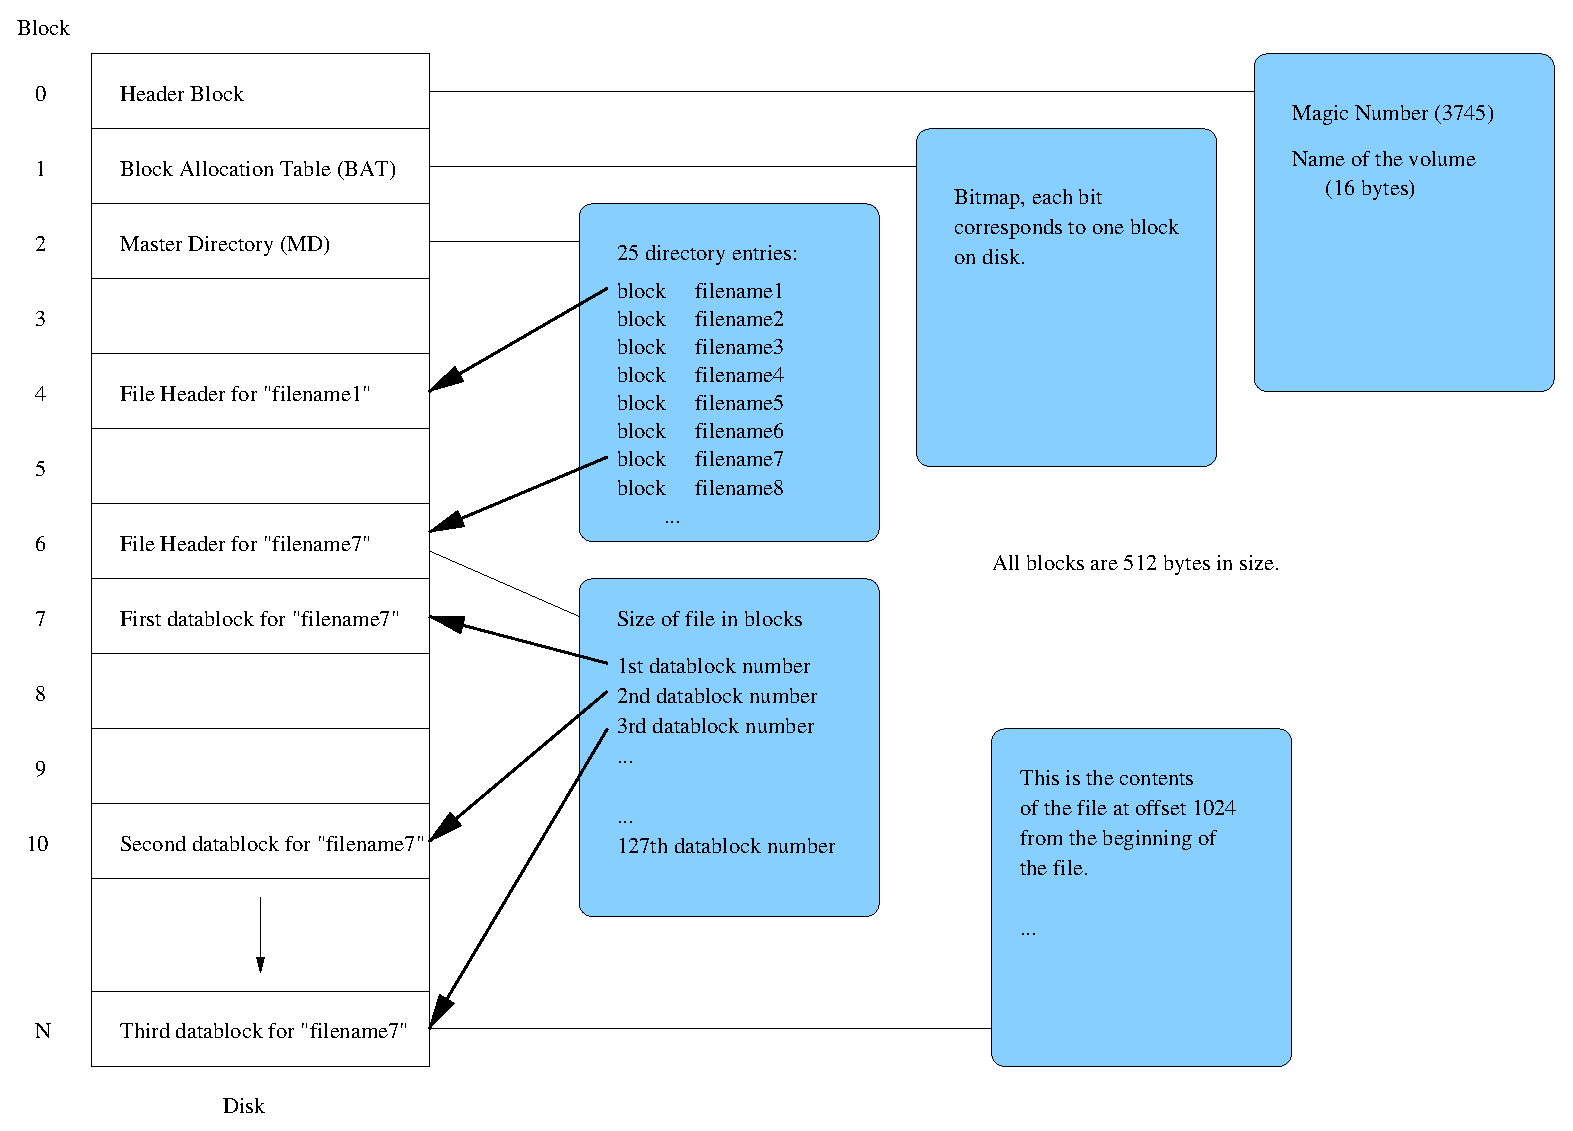
\includegraphics[width=\tablewidth,angle=0]{pics/tfs.eps}
\caption{Illustration of disk blocks on a TFS volume}
\label{fig:tfs}
\end{center}
\end{figure}

Note that all multibyte data in TFS is \emph{big-endian}. This is not
a problem in \buenos{}, since \yams{} is big-endian also, but must be
taken into consideration if you want to write e.g. TFS debugging tools
(native to the simulator platform).

The volume header block has the following structure. Other data may
be present after these fields, but it is ignored by TFS.

\begin{formatdescription}
\formatfield{0x00}{uint32\_t}{magic}{Magic number, must be 3745
(\texttt{0x0EA1}) for TFS volumes.}
\formatfield{0x04}{char [TFS\_VOLUMENAME\_ MAX]}{volname}{Name of the
volume, including the terminating zero.}
\end{formatdescription}


The block allocation table is a bitmap which records the free and
reserved blocks on the disk, one bit per block, 0 meaning free and 1
reserved. For a 512-byte block size, the allocation table can hold
4096 bits, resulting in a 2MB disk. Note that the allocation table
includes also the three first blocks, which are always reserved.

The master directory consists of a single disk block, containing a
table of the following 20-byte entries. This means that a disk with a
512-byte block size can have at most 25 files (512/20 = 25.6).


\begin{formatdescription}
\formatfield{0x00}{uint32\_t}{inode}{Number of the disk block
containing the file header (inode) of this file.}
\formatfield{0x04}{char [TFS\_FILENAME\_ MAX]}{name}{Name of the file,
including the terminating zero. This means that the maximum file name
length is actually TFS\_FILENAME\_MAX - 1.}
\end{formatdescription}

A file header block ("inode") describes the location of the file on
the disk and its actual size. The content of the file is stored to the
allocated blocks in the order they appear in the block list (the first
BLOCKSIZE bytes are stored to the first block in the list etc.). A
file header block has the following structure:

\begin{formatdescription}
\formatfield{0x00}{uint32\_t}{filesize}{Size of the file in bytes.}
\formatfield{0x04}{uint32\_t [TFS\_BLOCKS\_MAX]}{block}{Blocks
allocated for this file. Unused blocks are marked as 0 as a precaution
(since block 0 can never be a part of any file).}
\end{formatdescription}


With a 512-byte block size, the maximum size of a file is limited to
127 blocks ($512/4 - 1$) or 65024 bytes.

Note that this specification does not restrict the block size of the
device on which a TFS can reside. However, the \buenos{} TFS
implementation and the TFS tool do not support block sizes other than
512 bytes. Note also that even though the TFS filesystem size is
limited to 2MB, the device (disk image) on which it resides can be
larger, the remaining part is just not used by the TFS.


\subsection{TFS Driver Module}

The \buenos{} TFS module implements the Virtual File System interface
with the following functions.


\begin{function}{fs\_t *}{tfs\_init}{gbd\_t *disk}

\item Attempts to initialize a TFS on the given disk (a generic block
device, actually). If the initialization succeeds, a pointer to the
initialized filesystem structure is returned. If not (e.g. the header
block does not contain the right magic number or the block size is
wrong), NULL is returned.

\item Implementation:
\begin{enumerate}
\item Check that the block size of the disk is supported by TFS.
\item Allocate semaphore for filesystem locking (\texttt{tfs->lock}).
\item Allocate a memory page for TFS internal buffers and data and the
filesystem structure (\texttt{fs\_t}).
\item Read the first block of the disk and check the magic number.
\item Initialize the TFS internal data structures.
\item Store \texttt{disk} and the filesystem locking semaphore to the
internal data structure.
\item Copy the volume name from the read block into \texttt{fs\_t}.
\item Set \texttt{fs\_t} function pointers to TFS functions.
\item Return a pointer to the \texttt{fs\_t}.
\end{enumerate}

\end{function}



\begin{function}{int}{tfs\_unmount}{fs\_t *fs}

\item Unmounts the filesystem. Ensures that the filesystem is in a
``clean'' state upon exit, and that future operations will fail with
\texttt{VFS\_NO\_SUCH\_FS}.

\item Implementation:
\begin{enumerate}
\item Wait for active operation to finish by calling \texttt{semaphore\_P}
on \texttt{tfs->lock}.
\item Deallocate the filesystem semaphore \texttt{tfs->lock}.
\item Free the memory page allocated by \texttt{tfs\_init}.
\end{enumerate}

\end{function}


\begin{function}{int}{tfs\_open}{fs\_t *fs, char *filename}

\item Opens a file for reading and writing. TFS does not keep any
status regarding open files, the returned file handle is simply the
inode block number of the file.

\item Implementation:
\begin{enumerate}
\item Lock the filesystem by calling \texttt{semaphore\_P} on
\texttt{tfs->lock}.
\item Read the MD block.
\item Search the MD for \texttt{filename}.
\item Free the filesystem by calling \texttt{semaphore\_V} on
\texttt{tfs->lock}.
\item If \texttt{filename} was found the MD, return its inode block
number, otherwise return \texttt{VFS\_NOT\_FOUND}.
\end{enumerate}

\end{function}


\begin{function}{int}{tfs\_close}{fs\_t *fs, int fileid}

\item Does nothing, since TFS does not keep status for open files.

\end{function}


\begin{function}{int}{tfs\_create}{fs\_t *fs, char *filename, int size}

\item Creates a file with the given name and size (TFS files cannot be
resized after creation).

\item The file will contain all zeros after creation.

\item Implementation:
\begin{enumerate}
\item Lock the filesystem by calling \texttt{semaphore\_P} on
\texttt{tfs->lock}.
\item Check that the size of the file is not larger than the maximum
  file size that TFS can handle.
\item Read the MD block.
\item Check that the MD does not contain \texttt{filename}.
\item Find an empty slot in the MD, return error if the
directory is full.
\item Add a new entry to the MD.
\item Read the BAT block.
\item Allocate the inode and file blocks from BAT, and write the block
numbers and the filesize to the inode in memory.
\item Write the BAT to disk.
\item Write the MD to disk.
\item Write the inode to the disk.
\item Zero the content blocks of the file on disk.
\item Free the filesystem by calling \texttt{semaphore\_V} on
\texttt{tfs->lock}.
\item Return \texttt{VFS\_OK}.
\end{enumerate}

\end{function}


\begin{function}{int}{tfs\_remove}{fs\_t *fs, char *filename}

\item Removes the given file from the directory and frees the blocks
allocated for it.

\item Implementation:
\begin{enumerate}
\item Lock the filesystem by calling \texttt{semaphore\_P} on
\texttt{tfs->lock}.
\item Read the MD block.
\item Search the MD for \texttt{filename}, return error if not found.
\item Read the BAT block.
\item Read inode block.
\item Free inode block and all blocks listed in the inode from the BAT.
\item Clear the MD entry (set inode to 0 and name to an empty string).
\item Write the BAT to the disk.
\item Write the MD to disk.
\item Free the filesystem by calling \texttt{semaphore\_V} on
\texttt{tfs->lock}.
\item Return \texttt{VFS\_OK}
\end{enumerate}

\end{function}


\begin{function}{int}{tfs\_read}{fs\_t *fs, int fileid, void *buffer, int bufsize,\brtab int offset}

\item Reads at most \texttt{bufsize} bytes from the given file into
the given buffer. The number of bytes read is returned, or a negative
value on error. The data is read starting from given offset. If the
offset equals the file size, the return value will be zero.

\item Implementation:
\begin{enumerate}
\item Lock the filesystem by calling \texttt{semaphore\_P} on
\texttt{tfs->lock}.
\item Check that \texttt{fileid} is sane ($\ge3$ and not beyond the
end of the device/filesystem).
\item Read the inode block (which is \texttt{fileid}).
\item Check that the offset is valid (not beyond end of file).
\item For each needed block do the following:
  \begin{enumerate}
  \item Read the block.
  \item Copy the appropriate part of the block into the right place in
  \texttt{buffer}.
  \end{enumerate}
\item Free the filesystem by calling \texttt{semaphore\_V} on
\texttt{tfs->lock}.
\item Return the number of bytes \emph{actually} read.
\end{enumerate}

\end{function}


\begin{function}{int}{tfs\_write}{fs\_t *fs, int fileid, void *buffer, int datasize,\brtab int offset}

\item Writes (at most) \texttt{datasize} bytes to the given file. The
number of bytes actually written is returned. Since TFS does not
support file resizing, it may often be the case that not all bytes are
written (which should actually be treated as an error condition). The
data is written starting from the given offset.

\item Implementation:
\begin{enumerate}
\item Lock the filesystem by calling \texttt{semaphore\_P} on
\texttt{tfs->lock}.
\item Check that \texttt{fileid} is sane ($\ge3$ and not beyond the
end of the device/filesystem).
\item Read the inode block (which is \texttt{fileid}).
\item Check that the \texttt{offset} is valid (not beyond end of file).
\item For each needed block do the following:
  \begin{enumerate}
  \item If only part of the block will be written, read the block.
  \item Copy the appropriate part of the block from the right place in
  \texttt{buffer}.
  \item Write the block.
  \end{enumerate}
\item Free the filesystem by calling \texttt{semaphore\_V} on
\texttt{tfs->lock}.
\item Return the number of bytes \emph{actually} written.
\end{enumerate}

\end{function}


\begin{function}{int}{tfs\_getfree}{fs\_t *fs}

\item Returns the number of free bytes on the filesystem volume.

\item Implementation:
\begin{enumerate}
\item Lock the filesystem by calling \texttt{semaphore\_P} on
\texttt{tfs->lock}.
\item Read the BAT block.
\item Count the number of zeroes in the bitmap. If the disk is smaller
than the maximum supported by TFS, only the first appropriate number
of bits are examined (of course).
\item Get number of free bytes by multiplying the number of free blocks by
block size.
\item Free the filesystem by calling \texttt{semaphore\_V} on
\texttt{tfs->lock}.
\item Return the number of free bytes.
\end{enumerate}

\end{function}



\begin{filelist}

\file{fs/vfs.h, fs/vfs.c}{Virtual Filesystem implementation}

\file{fs/filesystems.h, fs/filesystems.c}{Available filesystems}

\file{fs/tfs.h, fs/tfs.c}{TFS implementation}

\end{filelist}



\begin{exercises}

\item[]
Note that your filesystem, and other exercises in this chapter, must
use a new disk. First, create a new disk device with a blocksize of
128 bytes by adding the entry defined in \autoref{sec:exampledisk}
into your \texttt{yams.conf}.

Generic hints: Do not modify TFS or \texttt{tfstool}, make copies and
name them for example SFS (student filesystem) and \texttt{sfstool}.
This way you can still use \texttt{tfstool} to transfer files to the
system's TFS volume and you only need to support filesystem creation
with your own tool. Note that you must compile SFS and
\texttt{sfstool} with the 128 byte blocksize (which is a configuration
definition in the filesystem header file). Remember to include correct
headers in your own tool (\texttt{sfs.h}, not \texttt{tfs.h}).

You don't have to make TFS comply to constraints given in this or any
other exercise, it is enough that your filesystem and VFS are correct.
You can still use the old disk for the TFS.

\cexercise{Improve the concurrency of the filesystem. Modify the
filesystem so that:
\begin{itemize}
  \item The same file may be read or written concurrently by any
  number of processes.

  \item All filesystem operations must be atomic and serializable.
  This means that all reads and writes must look like atomic
  operations, although in reality they are done concurrently. Thus for
  example when a thread writes to a file all readers see either the whole
  write or none of it.

  \item File deletion must work even when the file is open by one or
  more threads. If the file is deleted and it is currently open in
  some thread, only new opens on that file must fail and all already
  opened file handles must work until they are closed. The blocks on a
  disk are released only after the file is not open with any
  thread\footnote{Typical way to use temporary files is to first
  create the file, then open it and finally delete it. The removal
  will then be handled automatically when the process exits.}.
\end{itemize}
}

\cexercise{Create a filesystem with large files. Your filesystem must
support files up to the size of the disk and disks of any size up to 1
megabyte. Note that for future extensibility, do not make the block
pointer types any smaller than in TFS (let them be 32-bit wide). Note
also that retrieving a block from a disk takes quite a lot of time.
Make sure that your design is fast enough to be feasible.}

\cexercise{Make files extensible. If a file is written beyond its end,
the file is extended so much that the write is possible. This also
makes it possible to create files with length 0 and expand them as
needed.}

\cexercise{Implement directories. Directories can contain files and
other directories, forming a hierarchical namespace together with
mount-point identifiers. For example, a full pathname to shell could be
\texttt{[root]bins/sys/shell}.

Hints: Handle directories as files internally. Plan carefully how
concurrent access to directories is handled.}

\cexercise{Implement a kernel information filesystem. The filesystem
should be a virtual filesystem, which is not on any disk. It can be
mounted normally to any mountpoint. The filesystem should contain one
file per each process in the system and each file describes the
current status of the corresponding process. Status information should
include at least process ID, name of executable, memory usage and
current thread state (running, sleeping, ready for running). If you
have implemented userland threads, replace the thread state with the
number of threads the process currently runs.}

\cexercise{Improve the performance of your filesystem in the case of
many concurrent users. The typical ways to improve filesystem
performance are:

\begin{enumerate}

\item Implement a mechanism to use a part of system main memory as a
cache for disk blocks. Three main styles for doing this are:

\begin{itemize}

\item A fixed sized (but configurable) chunk of memory is used for caching.

\item All otherwise unused memory pages are used for caching.

\item The virtual memory system will treat cache pages and pages used
by programs equally. Note that cache page might be clean (read cache)
or dirty (write cache).

\end{itemize}

Evaluate these three alternatives and implement the one you
consider to be the best. You can of course use your own scheme if you
find it superior to all of these.

\item Implement an I/O-scheduler for disk access. The current method
of handling disk read and write requests is a strict FIFO. Implement a
better \texttt{disksched\_schedule()} function which will improve
system performance by:

\begin{itemize}

\item Taking into account the disk block number where the requests in the
queue are made on. The seeks of the disk read/write head take a lot of
time and much speed can be gained by considering its movement when
ordering requests.

\item Make sure that no request can ever completely starve.

\item If you have implemented a priority scheduler, consider also
using thread priorities as a parameter when ordering disk requests
(note that the disk scheduler is currently run in the context of the thread
which made the request).

\end{itemize}

\item Tune the filesystem so that it will try to place blocks that are
usually used sequentially close to each other (like blocks of one
file). Together with a good disk scheduler, this should also improve
overall performance.

\end{enumerate}

Write also a set of test programs which demonstrate the performance
improvements gained. Analyze the performance gains. You might need to
instrument the operating system to get measurable results out of
your test program runs.}

\end{exercises}


\chapter{Networking}
\label{sec:network}

\index{networking}
\index{network!layers}
\index{generic devices!network}
\index{GND}
\index{network!stack}

The implementation of \buenos{} networking is organized in
layers. Each layer adds some more functionality to the lower
layers. The device driver implementing the Generic Network Device
(GND) interface can be thought of as the bottommost layer of the
network stack. This layer issues commands to the network device and
handles interrupts generated by the device. The implementation of this
layer was left as an exercise to the students. The GND interface is
documented in \autoref{sec:gnd}. Some hints about implementing the
device driver are given in \autoref{sec:nic}.

Above the device driver layer resides the network frame layer
discussed in \autoref{sec:framelayer}. This layer abstracts the
possibly multiple GNDs found in the system. Packets are received from
all GNDs and forwarded further to the correct upper layer packet
handler.

Packet Oriented Protocol (POP) implements an abstraction
similar to the unix sockets. It allows packets sent by different
entities in the same machine to be distinguished. The implementation
of POP is further explained in \autoref{sec:pop}.

A stream oriented protocol is left as an exercise to the
students. This layer should add connections and reliability to the
services provided by POP. Some hints about the implementation of a
stream oriented protocol are given in \autoref{sec:sop}.

For more information on advanced networking topics, see
\cite{stallings} p. 699--707, 586--590 and 608--615.

\section{Network Services}
\label{sec:framelayer}

\index{NIC}

Frame layer transfers frames through (possible) multiple Network
Interface Cards (NIC) abstracted by GNDs. There is a receive service
thread for each GND and when a frame is received it is forwared to the
appropriate upper level frame handler. Frames given to be sent are
sent through the appropriate GND.

\index{network!addresses}
Network addresses in \yams{} are one word long (32 bits). There are
two kinds of special addresses:
\begin{itemize}

\item \emph{Addresses containing all zeros} are loopback addresses.
\index{loopback address, network} While sending they are pushed
immediately to the upper level frame handlers.

\item \emph{Addresses containing all ones} are broadcast addresses.
\texttt{broadcast address, network} These frames are sent through
all GNDs.

\end{itemize}

\index{network!frame}
\index{frame, network}
\index{network!payload}
\index{payload, network}
\index{header!network}
\index{network!header}

The frame consists of header and payload as described in
\autoref{tab:network_frame}. Frame size is limited by page size of the
virtual memory system. This is because there is no way of reserving
two consecutive memory pages and device drivers handle \emph{physical
addresses}. Payload size is therefore page size minus header size.


\begin{table}
\begin{structdescription}

\structfield{\small{network\_frame\_header\_t}}{header}{Header of the frame.}

\structfield{uint8\_t []}{payload}{Payload to be transferred.}

\end{structdescription}
\caption{Fields in structure \texttt{network\_frame\_t}}
\label{tab:network_frame}
\end{table}

The frame header consists of source and destination addresses and the
protocol identification for payload.  Source and destination addresses
belong to the frame header of \yams{} network devices, but the
protocol identification field is considered as payload by
\yams{}. The header is described in \autoref{tab:network_frame_header}.

\begin{table}
\begin{structdescription}

\structfield{network\_address\_t}{destination}{Destination address 
of the frame.}

\structfield{network\_address\_t}{source}{Source address of the frame.}

\structfield{uint32\_t}{protocol\_id}{The higher level protocol id for 
this frame.}

\end{structdescription}
\caption{Fields in structure \texttt{network\_frame\_header\_t}}
\label{tab:network_frame_header}
\end{table}


\subsubsection{Upper Level Protocols}

All upper level protocols are defined in a static table
\texttt{network\_protocols}\index{network\_protocols@\texttt{network\_protocols}}.
Table entry, defined as
\texttt{network\_protocols\_t}\index{network\_protocols\_t@\texttt{network\_protocols\_t}},
contains the following information:


\begin{structdescription}

\structfield{uint32\_t}{protocol\_id}{Typecode of the protocol.}

\structfield{frame\_handler\_t}{frame\_handler}{Pointer to the
function that will handle the payload of the frame.}

\structfield{void (*)(void)}{init}{Initialization function of the protocol.}

\end{structdescription}

\texttt{frame\_handler\_t}
\index{frame\_handler\_t@\texttt{frame\_handler\_t}} is a function type
which behaves like this:

\begin{function}{int}{frame\_handler}{network\_address\_t source,\brtab 
    network\_address\_t destination, uint32\_t protocol\_id,\brtab 
    void *payload}

\item Upper level handler for the frame (payload). Takes as parameters
source and destination addresses of the frame, protocol identification
of the frame and payload of the frame.

\end{function}

An initialization function \texttt{protocols\_init()} is
provided. Function calls initialization function for each protocol in
\texttt{network\_protocols} table.

\subsubsection{Initialization}

In network initialization all network devices are searched and
\texttt{network\_interfaces} table is set up. Also socket and protocol
initialization functions are called here. For each GND found a receive
service thread is started.

The following network initialization function is provided.

\begin{function}{void}{network\_init}{void}

\item Initializes networking code. Also calls initialization functions for
sockets and protocols. Starts a receive thread for each GND found.

\item Implementation:
\begin{enumerate}

\item Mark all entries as unused (gnd == NULL) in the network interface table.

\item Find all network interfaces by \texttt{device\_get}, get their
GNDs and store GNDs, addresses and MTUs in the table. For each MTU,
assert that it is smaller than page size (the page size is 4096
bytes).

\item Create and run a thread for each GND. All the threads will run
\texttt{network\_receive\_thread} with a pointer to the GND as the
argument.

\end{enumerate}

\end{function}

\subsubsection{Receive Service Thread}

\index{network!service thread}
\index{receive service thread, network}
\index{service thread, network}

For each network interface found a receive service thread is
started. The main job is to allocate memory for frames to be received
and when a frame is recieved call the \texttt{network\_receive()}
function. Each thread has one interface attached to it  (given as parameter)
and frames are received through it. 

The receive service thread is implemented as follows:

\begin{function}{void}{network\_receive\_thread}{uint32\_t interface}

\item Receives frames from the given network device ad
infinitum. Calls the function \texttt{network\_receive\_frame()} which
will call upper level frame handler.

\item Index to the \texttt{network\_interfaces} table is given as parameter.

\item Implementation:
\begin{enumerate}

\item Allocate a page for frame receiving. Assert errors.

\item Call \texttt{GND->receive}.

\item If a frame is succesfully received, call
\texttt{network\_receive\_frame()}.

\item Go back to step one.

\end{enumerate}

\end{function}

\begin{function}{static int}{network\_receive\_frame}{network\_frame\_t *frame}
\item Finds a frame handler for the appropriate upper level protocol
and calls it.

\item Implementation
\begin{enumerate}

\item Find the frame handler by calling
\texttt{protocols\_get\_frame\_handler()}. The protocol ID found from
frame is given as parameter.

\item If found call it and return its value. 

\item Else return zero as failure.

\end{enumerate}

\end{function}

Upper level frame handlers must free the page reserved for the frame by
calling \texttt{network\_free\_frame()}.

\subsubsection{Service API}

\index{network!service API}
\index{service API, network}

Following functions are provided as service API. Upper level protocols
may be implemented on top of these. 

\begin{function}{network\_address\_t}{network\_get\_source\_address}{int n}

\item Get the local address of the \texttt{n}th network interface. Returns 0
if no such interface exists.

\item Implementation:
\begin{enumerate}

\item Check that n $\geq$ 0 and smaller than
\texttt{CONFIG\_MAX\_GNDS}\index{CONFIG\_MAX\_GNDS@\texttt{CONFIG\_MAX\_GNDS}}.
If not, return 0.

\item Get the \texttt{n}th entry from the table. If GND is not NULL, return
the address, otherwise return 0.

\end{enumerate}

\end{function}


\begin{function}{network\_address\_t}{network\_get\_broadcast\_address}{void}

\item Gets the global broadcast address.

\item Implementation:
\begin{enumerate}
\item Return \texttt{0xffffffff}.
\end{enumerate}

\end{function}


\begin{function}{network\_address\_t}{network\_get\_loopback\_address}{void}

\item Gets the loopback address.

\item Implementation:
\begin{enumerate}
\item Return 0.
\end{enumerate}

\end{function}


\begin{function}{int}{network\_get\_mtu}{network\_address\_t local\_address}

\item Gets the MTU of a GND. The frame header (12 bytes) is decremented
from the size of the frame. If the broadcast address is given, minimum of
all GND's MTU is returned.

\item Implementation:
\begin{enumerate}

\item If broadcast address: go trough all GNDs and find the minimun MTU.

\item Else: find \texttt{local\_address} from the GND table and get the MTU.

\item If not found, return 0.

\item Return MTU - 12.
\end{enumerate}

\end{function}


\begin{function}{int}{network\_send}{network\_address\_t source,\brtab
network\_address\_t destination, uint32\_t protocol\_id,
int length,\brtab void *buffer}

\item Sends one packet to network. Blocks.

\item If the \texttt{source} is broadcast address, the frame is
  broadcast on all network interfaces (with the interface's address as
  source, of course).

\item Returns positive value on success and negative on failure. 

\item Implementation:
\begin{enumerate}

\item ASSERT that the \texttt{length} is smaller or equal to 4084
(page size - 12)

\item Allocates page for the packet with
\texttt{pagepool\_get\_physical\_page}. If page allocation fails,
return NET\_ERROR.

\item If \texttt{destination} is loopback, push frame to upper levels by
calling \texttt{network\_receive\_frame()} immediately and return.

\item If \texttt{source} is broadcast: for each interface, do the following
  steps using interface address as source. If the \texttt{source} is not
  broadcast do the following steps only once.

\item Find \texttt{source} address from GND table (local address).

\item If not found, return \texttt{NET\_DOESNT\_EXIST}.

\item Call \texttt{network\_send\_interface()}.

\item Return success or failure. Negative values indicate failure and
zero or positive values success.

\end{enumerate}

\end{function}

\begin{function}{static int}{network\_send\_interface}{int interface,\brtab
network\_address\_t destination, network\_frame\_t *frame}

\item Sends a frame through the given interface. This is a helper
function to ease handling in more complex functions.

\item Implementation
\begin{enumerate}

\item Get \texttt{gnd} from \texttt{network\_interfaces} table.
\item Call \texttt{gnd->send()}.

\end{enumerate}

\end{function}


\begin{function}{void}{network\_free\_frame}{void *frame}

\item Frees the given frame. Called from protocol-specific frame
  handler after the frame is handled.

\item Implementation:
\begin{enumerate}

\item Call \texttt{vm\_free\_page()}.

\end{enumerate}

\end{function}




\section{Packet Oriented Transport Protocol}
\label{sec:pop}
\index{Packet Oriented Protocol}
\index{POP}
\index{port numbers, POP}
\index{POP!port numbers}

Packet Oriented Protocol (POP) is very similar to
UDP. Port numbers are used to identify different entities on the same
machine. POP offers unreliable delivery from one entity on one machine
to another entity on another machine.

\index{sockets, network}
The port numbers are implemented by a socket abstraction which is very
similar to the sockets found in UNIX like operating systems. A socket
is bound to a port number which can be given explicitly when creating
the socket or it may be chosen randomly by \buenos{}. The
implementation of POP includes functions to open and close sockets and
to send and receive a packet through an opened socket. The socket
implementation is further discussed in \autoref{sec:sockets}.

POP also needs some structures and functions that are not essentially
a part of the socket abstraction. These include the format of a POP
packet and a queue for incoming packets. A thread which places the
incoming packets to correct receive buffers is also needed. These
issues and the implementation of the protocol specific functions of
the socket abstraction are discussed in \autoref{sec:popspecific}.

\subsection{Sockets}
\label{sec:sockets}
\index{sockets, network}

Open sockets are stored in a static size table called
\texttt{open\_sockets}\index{open\_sockets@\texttt{open\_sockets}}.
This table contains entries of the form \texttt{socket\_descriptor\_t}
\index{socket\_descriptor\_t@\texttt{socket\_descriptor\_t}} which is
described in \autoref{tab:socket}. The size of this table is
determined by
\texttt{CONFIG\_MAX\_OPEN\_SOCKETS}\index{CONFIG\_MAX\_OPEN\_SOCKETS@\texttt{CONFIG\_MAX\_OPEN\_SOCKETS}}.
The access to this table is synchronized by a semaphore,
\texttt{open\_sockets\_sem}\index{open\_sockets\_sem@\texttt{open\_sockets\_sem}}.

\begin{table}
\begin{structdescription}

\structfield{uint16\_t}{port}{The port that this socket is bound to.}

\structfield{uint8\_t}{protocol}{The protocol id of the protocol used
with this socket.}

\structfield{void *}{rbuf}{This is the address of the receive buffer
if some thread is currently waiting for input from this socket, NULL
if there is no waiting thread.}

\structfield{uint32\_t}{bufsize}{Size of the receive buffer. No
more than this number of bytes are copied to the buffer.}

\structfield{network\_address\_t *}{sender}{When a packet is received
  the sender's address is stored here.}

\structfield{int *}{copied}{When a packet is received, the number of
  copied bytes is stored here.}

\structfield{uint16\_t *}{sport}{When a packet is received, the port
  number of the sender is stored here.}

\end{structdescription}
\caption{Fields in structure \texttt{socket\_descriptor\_t}}
\label{tab:socket}
\end{table}

The socket implementation has three functions, \texttt{socket\_init},
\texttt{socket\_open} and \texttt{socket\_close}. In addition to
these, the POP implementation includes functions
\texttt{socket\_sendto} \index{socket\_sendto@\texttt{socket\_sendto}}
and
\texttt{socket\_recvfrom}\index{socket\_recvfrom@\texttt{socket\_recvfrom}}.
The stream-oriented transport protocol is left as an exercise to the
students. The implementation of this protocol should include functions
like
\texttt{socket\_connect}\index{socket\_connect@\texttt{socket\_connect}},
\texttt{socket\_read} \index{socket\_read@\texttt{socket\_read}},
\texttt{socket\_listen} \index{socket\_listen@\texttt{socket\_listen}}
and
\texttt{socket\_write}\index{socket\_write@\texttt{socket\_write}}.

\begin{function}{void}{socket\_init}{void}

\item Initializes the structures needed to implement the socket
abstraction.

\item Implementation:
\begin{enumerate}
\item Ensure that this function is called only once.
\item Initialize \texttt{open\_sockets\_sem} to 1 (free) and assert
  that the initialization succeeds.
\item Initialize all open sockets to empty (protocol 0).
\end{enumerate}
\end{function}

\begin{function}{sock\_t}{socket\_open}{uint8\_t protocol, uint16\_t port}
\item This function will create a socket and bind it to the given
port. A handle for the socket is returned.
\item \texttt{protocol} is 0x01 for POP.
\item \texttt{port} is the port to bind to. If set to 0, \buenos{} will
select a free port.

\item Implementation:
\begin{enumerate}
\item Check that \texttt{protocol} is one of the supported ones, return
error (-1) if not.
\item Call \texttt{semaphore\_P} on \texttt{open\_sockets\_sem}.
\item Find a free socket descriptor from the table. If the table was
full, call \texttt{semaphore\_V} on \texttt{open\_sockets\_sem} and
return error.
\item If \texttt{port} is 0, find the first unused port by looking through all
open sockets in the table.
\item Otherwise check that the port is unused. If the port is in use
  call \texttt{semaphore\_V} on \texttt{open\_sockets\_sem} and return error.
\item Save \texttt{protocol} and \texttt{port} into the table entry
  and initialize other fields to 0 or NULL.
\item Call \texttt{semaphore\_V} on \texttt{open\_sockets\_sem}.
\item Return the index to the socket table.
\end{enumerate}

\end{function}

\begin{function}{void}{socket\_close}{sock\_t socket}
\item This function unbinds the \texttt{socket} in question. The
socket can no longer be used after this.

\item Implementation:
\begin{enumerate}
\item Check that \texttt{socket} has a valid value.
\item Call \texttt{semaphore\_P} on \texttt{open\_sockets\_sem}.
\item Mark the entry in the socket table as unused by setting the
protocol to 0 and also zero all other fields.
\item Call \texttt{semaphore\_V} on \texttt{open\_sockets\_sem}.
\end{enumerate}

\end{function}

\subsection{POP-Specific Structures and Functions}
\label{sec:popspecific}
\index{POP}

\index{POP!header}
\index{header!POP}
POP defines its own packet format which is described in
\autoref{tab:poppacket}. The header includes the port values which are
used to distinguish different entities in a machine. The source and
destination network addresses are found in the lower level network
headers and are therefore not included in the POP header. POP allows
an application to send packets of length less or equal to the network
MTU (including all headers). To know where the data ends POP header
thus contains the SIZE field, which tells the payload data length in
bytes.

\begin{table}
\begin{center}

\begin{tabularx}{\tablewidth}{l|l|r|>{\PBS\raggedright}X}
\textbf{Offset} & \textbf{Name} & \textbf{Size} & \textbf{Description} \\
\hline
0 & SPORT & 2 & Source port; the sender is bound to this port.\\
\hline
2 & DPORT & 2 & Destination port; the receiver listens to (is bound
to) this port. \\
\hline
4 & SIZE & 4 & The size of the payload data in bytes. \\
\hline
8 & DATA & variable & The payload data, of length SIZE. \\
\end{tabularx}
\end{center}
\caption{POP packet format}
\label{tab:poppacket}
\end{table}

\index{queue, POP} \index{POP!queue} The main functionality of POP is
to send and receive packets. Sending in POP is done synchronously.
That is, the sending thread is used to send the packet so that no
packet queueing is needed. Receiving, however, needs to be done
asynchronously so POP contains a queue for received packets. The
structure of entries in the queue for received POP packets is
presented in \autoref{tab:popqueue}. The queue is of static length
defined by
\texttt{CONFIG\_POP\_QUEUE\_SIZE}\index{CONFIG\_POP\_QUEUE\_SIZE@\texttt{CONFIG\_POP\_QUEUE\_SIZE}}.
Access to the POP queue is protected by a semaphore,
\texttt{pop\_queue\_sem}\index{pop\_queue\_sem@\texttt{pop\_queue\_sem}}.

When a frame arrives, the \buenos{} network layer examines the
protocol number in the frame header and calls the appropriate frame
handler. The frame handler for POP is
\texttt{pop\_push\_frame}\index{pop\_push\_frame@\texttt{pop\_push\_frame}}.
This function will place the arrived packet to the POP queue. When POP
is initialized, a service thread is created. This thread continually
scans the POP queue and delivers packets to applications if they are
ready to receive packets.

\begin{table}
\begin{center}

\begin{structdescription}
\structfield{void *}{frame}{The received packet.}
\structfield{sock\_t}{socket}{The socket that will receive this packet.}
\structfield{uint32\_t}{timestamp}{The time when this packet was put
  to the queue.}
\structfield{network\_address\_t}{from}{The address of the sender.}
\structfield{int}{busy}{1 if this entry is in use, 0 otherwise.}
\end{structdescription}

\end{center}
\caption{Structure for entries in the pop queue.}
\label{tab:popqueue}
\end{table}

The POP implementation includes the following functions:

\begin{function}{void}{pop\_init}{void}
\item Initialize the POP layer by emptying the entries in the
\texttt{pop\_queue} and starting the POP service thread.

\item Implementation:
\begin{enumerate}
\item Ensure that this function is executed only once.
\item Assert that POP header has the correct lenght.
\item Allocate a page for the send buffer and assert that this
succeeds.
\item Create the three needed semaphores
  (\texttt{pop\_send\_buffer\_sem}, \\\texttt{pop\_queue\_sem} and
  \texttt{pop\_service\_thread\_sem}) and assert that this succeeds.
\item Initialize all entries in the \texttt{pop\_queue} to empty.
\item Start the service thread.
\end{enumerate}
\end{function}

\begin{function}{int}{pop\_push\_frame}{network\_address\_t fromaddr,
   \brtab network\_address\_t toaddr, uint32\_t protocol\_id, void *frame}

\item Place the frame into the POP frame queue and wake up the POP
service thread. If there is no space in the queue, return
0. \texttt{frame} points to the beginning of the page containing the
frame, and the frame will include the from and to addresses of the
frame layer (ie. it is in the full frame format).

\item \texttt{frame} is a page allocated by the caller (frame
layer). When the POP layer has no more need for the page it will call
\texttt{network\_free\_frame(frame)}.

\item Returns 1 if the frame was accepted (placed in the queue) and 0
if not. In case of return value 0, the caller may free or reuse the
frame immediately.

\item Implementation:
\begin{enumerate}
\item Check that the \texttt{protocol\_id} is POP.
\item Call \texttt{semaphore\_P} on \texttt{pop\_queue\_sem}.
\item Search the queue for an empty slot. If no empty slot was found,
find the oldest \emph{nonbusy} entry. If the oldest entry is younger
than
\texttt{CONFIG\_POP\_QUEUE\_MIN\_AGE}\index{CONFIG\_POP\_QUEUE\_MIN\_AGE@\texttt{CONFIG\_POP\_QUEUE\_MIN\_AGE}},
call V on \texttt{pop\_queue\_sem} and return 0.

\item For the selected entry, set the frame field to \texttt{frame},
socket field to -1, \texttt{from} to \texttt{fromaddr}, timestamp to
\texttt{rtc\_get\_msec} and busy to 0.

\item Call \texttt{semaphore\_V} on \texttt{pop\_queue\_sem}.

\item Call \texttt{semaphore\_V} on \texttt{pop\_service\_thread\_sem}
  to signal the POP service thread.

\item Return 1 to indicate that the frame was accepted.

\end{enumerate}

\end{function}

\begin{function}{void}{pop\_service\_thread}{uint32\_t dummy}

\item This function runs in its own thread delivering incoming POP
packets to right receive buffers and discarding packets whose
destination port is not listened. When there is nothing to do, the
service thread will wait on the \texttt{service\_thread\_sem}.

\item Implementation: repeat the following ad infinitum:
\begin{enumerate}

\item Call \texttt{semaphore\_P} on \texttt{open\_sockets\_sem}.
\item Call \texttt{semaphore\_P} on \texttt{pop\_queue\_sem}.

\item Find the first nonempty entry in the pop queue.

\item If its destination port is not listened, mark the queue entry as
empty and call \texttt{network\_free\_frame}. The call must be
postponed after the semaphore release because many semaphores are
held.

\item If the destination port is listened but no one is waiting for a
packet for that socket (receive buffer is NULL), find the next
nonempty frame and repeat from the previous step.

\item If the destination port is listened and someone is waiting for a
packet, mark the queue entry as busy and mark the frame (function
internal) to be transferred.

\item Call \texttt{semaphore\_V} on \texttt{pop\_queue\_sem}.
\item Call \texttt{semaphore\_V} on \texttt{open\_sockets\_sem}.

\item If a frame was marked to be discarded, call
\texttt{network\_free\_frame} and mark the row in the queue as unused.

\item If a frame was marked to be transferred, do the following:
\begin{enumerate}

\item Transfer the proper amount of POP payload bytes to the receive
buffer of the socket and set the \texttt{sender}, \texttt{sport} and
\texttt{copied} fields to corresponding values (sockets need not be
synchronized since no one should touch our socket when it is in waiting
state).

\item Mark the receive buffer for the socket as NULL.

\item Mark the queue entry as empty (no synchronization is needed here either,
since no one \emph{else} will touch busy entries).

\item Call \texttt{network\_free\_frame} for the frame.

\item Wake the thread waiting for the transfer to complete..
\end{enumerate}

\item If any frames were processed (transferred or freed), repeat from
step 1.

\item Call \texttt{semaphore\_P} on \texttt{pop\_service\_thread\_sem}.

\end{enumerate}

\end{function}

The following functions are actually part of the socket interface but
they are implemented by POP.

\begin{function}{int}{socket\_sendto}{sock\_t s, network\_address\_t
    addr, uint16\_t dport,\brtab void *buf, int size}
\item Send \texttt{size} bytes from buffer \texttt{buf} to address
\texttt{addr}, port \texttt{dport}, using socket \texttt{s}.

\item Implementation:
\begin{enumerate}
\item Check that \texttt{s}, \texttt{size} and \texttt{buf} are sane,
return error (-1) if not.
\item Limit \texttt{size} so that the whole frame will fit into one
page.
\item Call \texttt{semaphore\_P} on \texttt{open\_sockets\_sem}.
\item Check that the given socket is a POP socket.
\item Copy the entry indexed by \texttt{s} to a local variable.
\item Call \texttt{semaphore\_V} on \texttt{open\_sockets\_sem}.
\item Call \texttt{semaphore\_P} on \texttt{pop\_send\_buffer\_sem}.
\item Fill the POP header located at the start of
\texttt{pop\_send\_buffer} with PRID=0x01, RSRVD=0x00, SPORT=port from
the socket entry, and DPORT=dport.
\item Move \texttt{size} bytes from \texttt{buf} to the data area in
the POP packet.
\item Call \texttt{network\_send} using broadcast address as source
  address so that the packet will be sent through all network
  interfaces.
\item Call \texttt{semaphore\_V} on \texttt{pop\_send\_buffer\_sem}.
\item Return the number of payload bytes sent or error if
\texttt{network\_send} returned error.
\end{enumerate}

\end{function}

\begin{function}{int}{socket\_recvfrom}{sock\_t s, network\_address\_t
    *addr,\brtab uint16\_t *sport, void *buf, int maxlength, int *length}
\item Receive at most \texttt{maxlength} bytes from network using
socket \texttt{s}, storing the received data into buffer
\texttt{buf}. The sender's address is stored in \texttt{*addr}. The
number of actually received bytes is stored in \texttt{*length}.

\item Implementation:
\begin{enumerate}

\item Check that the parameters are sane.

\item Call \texttt{semaphore\_P} on \texttt{open\_sockets\_sem}.

\item If the \texttt{rbuf} field of the socket is not NULL, release the
semaphore and return -1 (someone else is waiting for a packet for the
same socket, this is not supported). Also check that this is a POP
socket.

\item Set the fields \texttt{rbuf}, \texttt{bufsize}, \texttt{sender},
\texttt{sport} and \texttt{copied} for \texttt{s} from the arguments.

\item Call \texttt{semaphore\_V} on \texttt{open\_sockets\_sem}.

\item Wake up the POP service thread by calling \texttt{semaphore\_V}
  on the semaphore \texttt{pop\_service\_thread\_sem}.

\item Wait until the packet has been transfered by calling
\texttt{semaphore\_P} on \texttt{receive\_complete} semaphore in the
socket structure.

\item Return the number of bytes received.

\end{enumerate}

\end{function}


\section{Stream Oriented Protocol API}
\label{sec:sop}

\index{SOP}
\index{Stream Oriented Protocol}
\index{connection oriented protocol}

The existing network implementation doesn't support connection
oriented reliable sockets. This kind of sockets provide reliable
communication on unreliable network and can transfer arbitrary number
of bytes on single connection. The interface (for non-exisisting
protocol) to stream sockets is following (see also
\texttt{net/sop.h}):

\begin{function}{int}{socket\_connect}{sock\_t s, network\_address\_t addr,
int port}

\item Connects to remote machine (address \texttt{addr}) at port
\texttt{port}. The connection remains open until explicitly closed by
call to \texttt{socket\_close()} or connection is lost.

\item Return 0 on success, 1 on failure.

\end{function}

\begin{function}{void}{socket\_listen}{sock\_t s}

\item Waits until given socket \texttt{s} has been connected by
someone (listen on server socket).

\end{function}

\begin{function}{int}{socket\_read}{sock\_t s, void *buf, int length}

\item Reads at most \texttt{length} bytes from given socket \texttt{s}.
The data read is written to buffer \texttt{buf}.

\item Returns the number of bytes read. Zero indicates end of stream
and negative values are returned on errors.

\end{function}

\begin{function}{int}{socket\_write}{sock\_t s, void *buf, int length}

\item Writes \texttt{length} bytes to given socket \texttt{s}. The data
is read from buffer \texttt{buf}.

\item Returns the number of bytes successfully delivered to the destination.
If the return value is not equal to \texttt{length}, an unrecoverable error
has occured and the socket connection is lost.

\end{function}

\begin{filelist}

\file{net/network.h, net/network.c}{Network frame layer}

\file{net/protocols.h, net/protocols.c}{List of available network protocols}

\file{net/socket.h, net/socket.c}{Socket library}

\file{net/pop.h, net/pop.c}{Packet oriented unreliable networking protocol}

\file{net/sop.h}{Stream oriented reliable networking protocol API
(no implementation available)}

\end{filelist}

\begin{exercises}

\cexercise{Implement a reliable stream oriented network protocol. The
interface to the protocol is described in \autoref{sec:sop}.}

\cexercise{Implement a network filesystem. The filesystem should be
mountable to the standard VFS interface (see \autoref{sec:vfs}). The
server side implementation must support multiple simultaneous clients
on the same filesystem at the same time. Userland programs must be
able to use network filesystem just like a local filesystem.}

\cexercise{Implement process migration through network. Any userland
process must be able to call new system call (you define it) and give
an address of a target machine. The process is then migrated into that
new machine. All already open files must work normally after the
migration, but console prints will go to the console of the new host
machine. The process can re-migrate at any time it wishes.}

\end{exercises}




\chapter{Device Drivers}
\label{sec:device}
\index{device drivers}
\index{devices}

Since \buenos{} runs on a complete simulated machine, it needs to be
able to access the simulated devices in \yams{}. These hardware
devices include system consoles, disks and network interface adapters.
Device drivers use two hardware provided mechanisms intensively: they
depend on hardware generated interrupts and command the hardware with
memory mapped I/O.

Most hardware devices generate interrupts when they have completed the
previous action or when some asynchronous event, such as arrival of a
network frame, occurs. Device drivers implement handlers for these
interrupts and react to the event.

\index{DMA}
\index{memory!mapped I/O}
Memory mapped I/O is an interface to the hardware components. The
underlying machine provides certain memory addresses which are
actually ports in hardware. This makes it possible to send and receive
data to and from hardware components. Certain components also support
block data transfers with direct memory access (DMA). In DMA the data
is copied between main memory and the device without going through
CPU. Completion of DMA transfer usually causes an interrupt.

\index{top half, device driver}
\index{bottom half, device driver}
\index{shared IRQ}
\index{IRQ, shared}
Interrupt driven device drivers can be thought to have two halves, top
and bottom. The top half is implemented as a set of functions which
can be called from threads to get service from the device. The bottom
half is the interrupt handler which is run asynchronously whenever an
interrupt is generated by the device. It should be noted that the
bottom half might be called also when the interrupt was actually
generated by some other device which shares the same interrupt request
channel (IRQ).

Top and bottom halves of a device driver typically share some data
structures and require synchronized access to that data. The threads
calling the service functions on the top half might also need to sleep
and wait for the device. Resource waiting (also called blocking or
sleeping) is implemented by using the sleep queue or semaphores. The
syncronization on the data structures however needs to be done on a
lower level since interrupt handlers cannot sleep and wait for access
to the data. Thus the data structures need to be synchronized by disabling
interrupts and acquiring a spinlock which protects the data. In
interrupt handlers interrupts are already disabled and only spinlock
acquiring is needed.

For an introduction on device drivers and hardware, read either
\cite{tanenbaum} p. 269--300 and 327--341 or \cite{stallings} p. 474--486.

\section{Interrupt Handlers}
\label{sec:inthandlers}
\index{interrupt!handler}

All device drivers include an interrupt handler. When an interrupt
occurs the system needs to know which interrupt handlers need to be
called. This mechanism is implemented with an interrupt handler
registration scheme. When the device drivers are initialized, they
will register their interrupt handler to be called whenever
specified interrupts occur. When an interrupt occurs, the interrupt
handling mechanism will then call all interrupt handlers which are
registered with the occured interrupt. This means that the interrupt
handler might be called although the device has not generated an
interrupt.

\index{registering interrupt handlers}

The registered interrupt handlers are kept in the table
\texttt{interrupt\_handlers} which holds elements of type
\texttt{interrupt\_entry\_t}. The fields of this structure are
described in the \autoref{tab:interruptentry}.

\begin{table}
\begin{structdescription}

\structfield{device\_t}{device}{The device for which this interrupt is
registered.}

\structfield{uint32\_t}{irq}{The interrupt mask. Bits 8 through 15
  indicate the interrupts that this handler is registered for. The
  interrupt handler is called whenever at least one of these
  interrupts has occured.}

\structfield{void (*)(device\_t *)}{handler}{The interrupt handler
  function called when an interrupt occurs. The argument given to
  this function is \texttt{device}.}

\end{structdescription}
\caption{Fields in structure \texttt{interrupt\_entry\_t}}
\label{tab:interruptentry}
\end{table}

\begin{function}{void}{interrupt\_register}{uint32\_t irq, void
    (*handler)(device\_t *),\brtab device\_t device}
\item Registers an interrupt handler for the \texttt{device}.
  \texttt{irq} is an interrupt mask, which indicates the interrupts
  this device has registered. Bits 8 through 15 indicate the registered
  interrupts. \texttt{handler} is the interrupt handler called when at
  least one of the specified interrupts has occured. This function can
  only be called during booting.
\item Implementation:
\begin{enumerate}
\item Find the first unused entry in \texttt{interrupt\_handlers}.
\item Insert the given parameters to the found table entry.
\end{enumerate}
\end{function}

\begin{function}{void}{interrupt\_handle}{uint32\_t cause}
\item Called when an interrupt has occured. The argument
  \texttt{cause} contains the Cause register. Goes through the
  registered interrupt handlers and calls those interrupt handlers
  that have registered the occured interrupt.
\item Implementation:
\begin{enumerate}
\item Clear software interrupts.
\item Call the appropriate interrupt handlers.
\item Call the scheduler if appropriate.
\end{enumerate}
\end{function}

\begin{filelist}
\file{kernel/interrupt.h, kernel/interrupt.c}
  {\texttt{interrupt\_entry\_t}, \texttt{interrupt\_register},
  \texttt{interrupt\_handle}}
\end{filelist}

\section{Device Abstraction Layers}
\label{sec:deviceabs}

\index{device abstraction layers}
\index{generic devices}

The device driver interface in \buenos{} contains several abstraction
layers. All device drivers must implement standard interface functions
(initialization function and possibly interrupt handler) and most will
also additionally implement functions for some generic device type.
Three generic device types are provided in \buenos{}: generic
character device, generic block device and generic network device.
These can be thought as ''superclasses'' from which the actual device
drivers are inherited. The hierarchy of device driver abstractions is
shown in \autoref{fig:device}.

\begin{figure}
\begin{center}
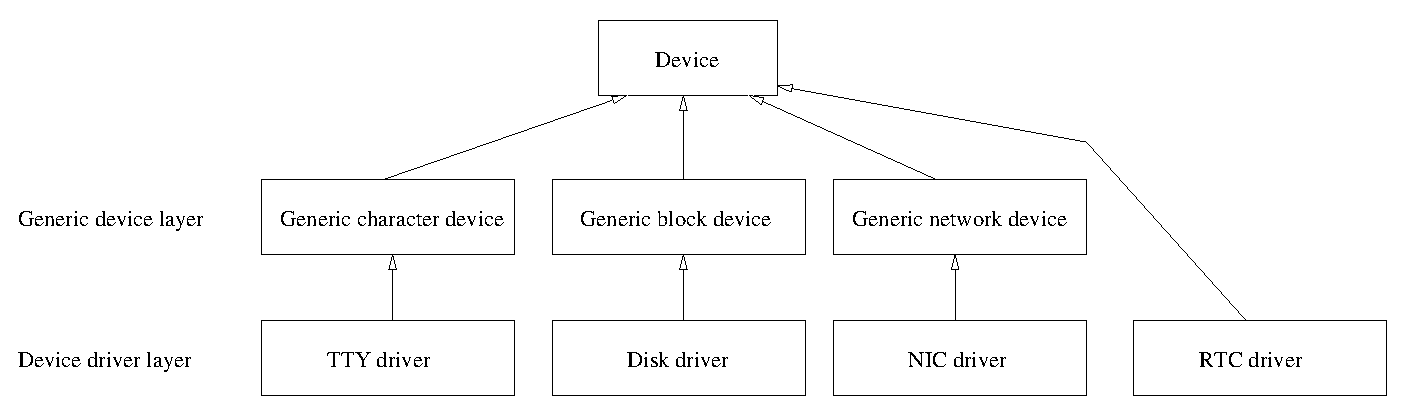
\includegraphics[width=\tablewidth,angle=0]{pics/device.eps}
\caption{\buenos{} device abstraction layers.}
\label{fig:device}
\end{center}
\end{figure}

Generic character device is a device which provides uni- or
bidirectional bytestream. The only such device preimplemented in
\buenos{} is the console. Generic block device is a device which
provides random read/write access to fixed sized blocks. The only such
device implemented is the disk driver. These interfaces could also be
used to implement stream based network protocol or network block
device, for example. The interface for generic network device is also
given. However there is no device driver implementing this interface
since the network device driver is left as an exercise.

All device drivers must have an initialization function. Pointer to
this function is placed in a structure \texttt{drivers\_available}
\index{drivers\_available@\texttt{drivers\_available}} in
\texttt{drivers/drivers.c} together with a device typecode identifier.
The system will initialize the device drivers in bootup for each
device in the system by calling these initialization functions. This
initialization is done in \texttt{device\_init()}.

\subsection{Device Driver Implementor's Checklist}
\label{sec:checklist}

\index{device drivers!implementing new ones}
\index{implementing a device driver}

When implementing a new device driver for \buenos{} at least the
following things must be done:

\begin{enumerate}
\item Place new driver in \texttt{drivers/}.
\item Implement functions which provide interface to the device for
threads. If possible, use generic device abstractions.
\item Implement interrupt handler for the device.
\item Implement initialization function which will allocate and
initialize device structure and register the interrupt handler.
\item Put the device driver's initialization function in
\texttt{drivers\_available} table in \texttt{drivers/drivers.c}.
\item Use \texttt{volatile} \index{volatile@\texttt{volatile}} keyword
  in the variable declarations that can be changed during the
  execution of a thread (e.g., when the process is sleeping,
  interrupted, $\ldots$). (The \texttt{volatile} keyword tells the
  compiler that the variable in question can be changed without any
  action taken by the code nearby the variable.)
\end{enumerate}

\subsection{Device Driver Interface}

Device driver initialization functions are placed in table
\texttt{drivers\_available}\index{drivers\_available@\texttt{drivers\_available}}.
The structure of an entry in that table is shown in
\autoref{tab:driversavailablet}.

\begin{table}
\begin{structdescription}

\structfield{uint32\_t}{typecode}{The typecode of the device this
  driver is intended for.}

\structfield{const char *}{name}{The name of this driver. Printed to
  console before the driver is initialized.}

\structfield{device\_t * (*)(io\_descriptor\_t
  *descriptor)}{initfunc}{A pointer to the initialization function for
  the driver. Starts the driver for the hardware device described by
  \texttt{descriptor} and return pointer to the device driver
  instance.}

\end{structdescription}
\caption{Fields in structure \texttt{drivers\_available\_t}}
\label{tab:driversavailablet}
\end{table}

Every device driver's initialization function must return a pointer to
device descriptor
(\texttt{device\_t}\index{device\_t@\texttt{device\_t}}) for this
device. The descriptor structure is explained in
\autoref{tab:devicet}.

\begin{table}
\begin{structdescription}

\structfield{void *}{real\_device}{Pointer to the device driver's internal
data structures.}

\structfield{void *}{generic\_device}{Pointer to a generic device
handle (generic character device, generic network device or generic
block device). Will be NULL if the device driver does not implement
any generic device interface.}

\structfield{io\_descriptor\_t *}{descriptor}{Pointer to the device
descriptor for the hardware device in device descriptor area provided
by \yams{}}

\structfield{uint32\_t}{io\_address}{Start address of the
memory-mapped I/O-area of the device.}

\structfield{uint32\_t}{type}{The typecode of this device. Typecodes
are listed in \texttt{drivers/yams.h}}

\end{structdescription}
\caption{Fields in structure \texttt{device\_t}}
\label{tab:devicet}
\end{table}

The device entry has a field of type \texttt{io\_descriptor\_t
*}\index{io\_descriptor\_t@\texttt{io\_descriptor\_t}}. This refers to
device descriptor record provided by the hardware (\yams{}). This
structure is thus not allocated, but just referenced from hardware
device descriptor area in memory. The fields are documented in detail
in \yams{}'s manual, but are also shown in \autoref{tab:iodescriptort}.

\begin{table}
\begin{structdescription}

\structfield{uint32\_t}{type}{Typecode of the device.}

\structfield{uint32\_t}{io\_area\_base}{Start address of the device's
memory mapped I/O area.}

\structfield{uint32\_t}{io\_area\_len}{Lenght of the device's memory
mapped I/O area in bytes.}

\structfield{uint32\_t}{irq}{The interrupt request line used by this
device. \texttt{0xffffffff} if the device doesn't use interrupts.}

\structfield{char}{vendor\_string}{Vendor string of the device. Note
that the string is not 0-terminated.}

\structfield{uint32\_t[2]}{resv}{Reserved for future extensions.}

\end{structdescription}
\caption{Fields in \yams{} device descriptor structure
\texttt{io\_descriptor\_t}.}
\label{tab:iodescriptort}
\end{table}

In system boot-up, device driver initialization code is called from
\texttt{init()}. The function called is:

\begin{function}{void}{device\_init}{void}
\item Finds all devices connected to the system and attempts to initialize
device drivers for them.
\item Implementation:
\begin{enumerate}
\item Loop through the device descriptor area of \yams{}.
\item For each found device try to find the driver by scanning through
the list of available drivers (\texttt{drivers\_available in
\texttt{drivers/drivers.c}}).
\item If a matching driver is found, call its initialization function
and print the match to the console. Store the initialized driver
instance to the device driver table \texttt{device\_table}.
\item Else print a warning about an unrecognized device.
\end{enumerate}
\end{function}

After device drivers are initialized, we must have some mechanism to
get a handle of a specific device. This can be done with
the \texttt{device\_get} function\footnote{If you are familiar with
Unix device driver interface, it may help to think of the
\texttt{typecode} as major device number and \texttt{n} as minor
device number.}:

\begin{function}{device\_t *}{device\_get}{uint32\_t typecode, uint32\_t n}
\item Finds initialized device driver based on the type of the device
and sequence number. Returns Nth initialized driver for device with
type \texttt{typecode}. The sequencing begins from zero. If device
driver matching the specifield type and sequence number if not found,
the function returns \texttt{NULL}.
\end{function}

\subsection{Generic Character Device}
\label{sec:gcd}

\index{GCD}
\index{generic devices!character}

A generic character device (GCD) is an abstraction for any
character-buffered (stream based) I/O device (e.g. a terminal). A GCD
specifies read and write functions for the device, which have the same
syntax for every GCD. Thus, when using GCD for all character device
implementations, the code which reads or writes them does not have to
care whether the device is e.g. a TTY or some other character device.

The generic character device is implemented as a structure with the
fields described in the \autoref{tab:gcdt}.

\begin{table}
\begin{center}
\begin{tabularx}{\tablewidth}{p{3.5cm}|l|>{\PBS\raggedright}X}
\textbf{Type}     & \textbf{Name}    & \textbf{Explanation} \\
\hline

device\_t * & device & Pointer to the ``real'' device. \\

\hline

int (*)(gcd\_t * gcd, const void * buf, int len)  & write & Pointer to a
function which writes \texttt{len} bytes from \texttt{buf} to the
device. The function returns the number of bytes successfully written.
\\

\hline

int (*)(gcd\_t * gcd, void * buf, int len) & read & Pointer to a
function which reads at most \texttt{len} bytes to \texttt{buf} from
the device. The function returns the number of bytes successfully
read. \\

\end{tabularx}
\end{center}
\caption{Generic Character Device (\texttt{gcd\_t})}
\label{tab:gcdt}
\end{table}


\subsection{Generic Block Device}
\label{sec:gbd}

\index{generic devices!block}
\index{GBD}

Generic block device (GBD) is an abstraction of a block-oriented
device (e.g. disk). GBD consists of function interface and a
\emph{request} data structure that abstracts the blocks to be handled.
All functions are implemented by the actual device driver. Function
interface is provided as the \texttt{gbd\_t}
\index{gbd\_t@\texttt{gbd\_t}} (see \autoref{tab:gbdt}) data
structure.

\begin{table}
\begin{structdescription}

\structfield{device\_t *}{device}{Pointer to the actual device.}

\structfield{int (*)(gbd\_t * gbd, gbd\_request\_t
*request}{read\_block}{A pointer to a function which reads a
\texttt{request->block} from the device \texttt{gbd} to the buffer
\texttt{request->buf}. Before calling, fill the fields \texttt{block},
\texttt{buf} and \texttt{sem} in \texttt{request}. The call of this
function is synchronous if \texttt{sem} is NULL. The call of this
function is asynchronous otherwise. When the asynchronous read is done
the semaphore \texttt{sem} is signaled. In synchronous mode the return
value 1 indicates success and 0 failure. In asynchronous mode 1 is
returned when the work is submitted to the lower layer, 0 indicates
failure in submission.}

\structfield{int (*)(gbd\_t *gbd, gbd\_request\_t
*request}{write\_block}{A pointer to a function which writes a
\texttt{request->block} to the device \texttt{gbd} from the buffer
\texttt{request->buf}. Before calling, fill the fields \texttt{block},
\texttt{buf} and \texttt{sem} in \texttt{request}. The call of this
function is synchronous if \texttt{sem} is NULL. The call of this
function is asynchronous otherwise. When the asynchronous write is
done the semaphore \texttt{sem} is signaled. In synchronous mode the
return value 1 indicates success and 0 failure. In asynchronous mode 1
is returned when the work is submitted to the lower layer, 0 indicates
failure in submission.}

\structfield{uint32\_t (*)(gbd\_t * gbd)}{block\_size}{Returns the
block size of the device in bytes.}

\structfield{uint32\_t (*)(gbd\_t * gbd)}{total\_blocks}{Returns the
total number of blocks on the device.}

\end{structdescription}
\caption{Fields in the structure \texttt{gbd\_t}.}
\label{tab:gbdt}
\end{table}

Blocks to be handled are abstracted by the \texttt{gbd\_request\_t}
\index{gbd\_request\_t@\texttt{gbd\_request\_t}} data structure
(\autoref{tab:requestt}). Structure includes all necessary information
related to the reading or writing of a block.

\begin{table}
\begin{structdescription}

\structfield{\texttt{gbd\_operation\_t}}{operation}{Read or write. Set
when write or read is called, preset values are ignored.}

\structfield{\texttt{uint32\_t}}{\texttt{block}}{Block number to operate on.}

\structfield{\texttt{uint32\_t}}{\texttt{buf}}{Non mapped address
(physical memory address) to a buffer of size equal to blocksize of
the device. Address must be a physical memory address, because physical
devices will handle only those.}

\structfield{\texttt{sem\_t *}}{\texttt{sem}}{Semaphore which will be
incremented when the request is done. Can be \texttt{NULL}. If
\texttt{NULL}, the request will be handled synchronously (will
block).}

\structfield{\texttt{void *}}{\texttt{internal}}{Driver internal 
information, ignored when using this structure.}

\structfield{\texttt{gbd\_request\_t *}}{\texttt{next}}{Pointer to
the next request in the chain. Ignore when using, driver will use this in
the I/O-scheduler.}

\structfield{\texttt{int}}{\texttt{return\_value}}{Return status of
this request.  Set when request is handled. This is 0 if the request
was successful.}

\end{structdescription}
\caption{Fields in the structure \texttt{gbd\_request\_t}.}
\label{tab:requestt}
\end{table}

The \texttt{gbd\_operation\_t}
\index{gbd\_operation\_t@\texttt{gbd\_operation\_t}} is an enumeration
of following values: \texttt{GBD\_OPERATION\_READ}
\index{GBD\_OPERATION\_READ@\texttt{GBD\_OPERATION\_READ}} and
\texttt{GBD\_OPERATION\_WRITE}\index{GBD\_OPERATION\_WRITE@\texttt{GBD\_OPERATION\_WRITE}}.

In case of asynchronous calls \emph{gbd}-interface functions will
return immediately and waiting is left for the caller. This means
creating a semaphore before submitting the request and the waiting it
to be released. Memory reserved for the request may not be released
until the \emph{request} is really served by the interrupt handler
(ie. semaphore is released). The thread using a GBD device must be
very careful especially with reserving memory from function stacks
(ie. static allocation). If function is exited before the
\emph{request} is served, memory area of the request may corrupt.

In case of synchronous calls \emph{gbd}-inerface functions will block
until the request is handled. The memory of the \emph{request} data
structure may be released when returned from \emph{gbd}-interface
functions.


\subsection{Generic Network Device}
\label{sec:gnd}
\index{GND}
\index{generic devices!network}

A generic network device (GND) is an abstraction of any network
device. The GND interface defines functions for receiving and sending
data as well as finding the maximum transfer unit (MTU) or the network
address of the interface. GND is a generic interface which allows the
code that uses the network device to be unaware of the actual
implementation of the network device driver. The GND structure is
described in \autoref{tab:gndt}. \index{gnd\_t@\texttt{gnd\_t}}

\begin{table}
\begin{structdescription}

\structfield{device\_t *}{device}{Pointer to the real device.}

\structfield{int (*)(struct gnd\_struct *gnd, void *frame,
network\_address\_t addr)}{send}{Pointer to a function which sends one
network frame to the given address. The network frame must be in the
format defined by the media. (For \yams{} this means that the first 8
octets are filled by the network layer and the rest is data.) The call
of this function blocks until the frame is sent. Note that the pointer
to the frame is a physical address, not a segmented one and the frame
must have the size returned by the \texttt{frame\_size} function. The
return value 0 means success. Other values indicate failure.}

\structfield{int (*)(struct gnd\_struct *gnd, void
*frame)}{recv}{Pointer to a function which receives one network frame.
The network frame returned will be in the format defined by the media.
(For \yams{} this means that the first 8 octets specify the source and
destination addresses and the rest is data.) Note that the pointer to
the frame is a physical address, not a segmented one and the frame
must have the size returned by the \texttt{frame\_size} function. The
call of this function will block until a frame is received. Otherwise
the call will return error when no frame is available. The return
value 0 means success. Other values indicate failure.}

\structfield{uint32\_t (*)(struct gnd\_struct
  *gnd)}{frame\_size}{Pointer to a function which returns the frame
  size of the media in octets.}

\structfield{network\_address\_t (*)(struct gnd\_struct
*gnd)}{hwaddr}{Pointer to a function which returns the network address
(MAC) of this interface.}

\end{structdescription}
\caption{Fields in the structure \texttt{gnd\_t}.}
\label{tab:gndt}
\end{table}

\begin{filelist}
\file{drivers/device.h, drivers/device.c}{Device driver interface}
\file{drivers/drivers.h, drivers/drivers.c}{List of available device drivers}
\file{drivers/yams.h}{Constants derived from the \yams{} hardware}
\file{drivers/gcd.h}{Generic character device}
\file{drivers/gbd.h}{Generic block device}
\file{drivers/gnd.h}{Generic network device}
\end{filelist}


\section{Drivers}

\subsection{Polling TTY driver}
\label{sec:polltty}

\index{polling TTY driver}
\index{driver!polling TTY}

Two separate drivers are provided for TTY. The first one is
implemented by polling and the other with interrupt handlers. The
polling driver is needed in boot up sequence when interrupts are
disabled. It is also useful in kernel panic situations, because
interrupt handlers might not be relied on in error cases.

\begin{function}{void}{polltty\_init}{void}
\item Initializes the polling TTY driver. Finds the first console
device in YAMS and attaches to that. Other \texttt{polltty}-functions must not
be called before \texttt{polltty\_init()} has been called.
\end{function}

\begin{function}{int}{polltty\_getchar}{void}
\item Gets one character from TTY device. Blocks (busyloop) until a
character has been successfully read. Returns 0 on error (no TTY
device).
\item Returns the character read.
\item Note that the polling TTY driver is unreliable on reads:
characters may be lost if input buffer overflows in the hardware (buffer
is 1 character in size).
\end{function}

\begin{function}{void}{polltty\_putchar}{char c}
\item Writes character \texttt{c} to TTY. If TTY is not initialized or
found, ignores the write.
\end{function}


\begin{filelist}
\file{drivers/polltty.c, drivers/polltty.h}{Polling TTY driver implementation}
\file{lib/libc.c, lib/libc.h}{\texttt{kwrite()} and \texttt{kread()}}
\end{filelist}


\subsection{Interrupt driven TTY driver}

\index{interrupt!TTY driver}
\index{driver!interrupt driven TTY}

The interrupt driven or the \emph{asynchronous} TTY driver is the
terminal device driver used most of the kernel terminal I/O-routines.
The terminal driver has two functions to provide output to the terminal
and input to the kernel. Both of these happen asynchronously. I.e.,
the input handling is triggered when the user presses a key on the
keyboard. The output handler is invoked when some part of the kernel
requests a write. The asynchronous TTY driver is implemented in
\texttt{drivers/tty.c} and implements the generic character device
interface.

The following functions implement the TTY driver:

\begin{function}{device\_t *}{tty\_init}{io\_descriptor\_t *desc}
\item Initialize a driver for the TTY defined by \texttt{desc}.
  This function is called once for each TTY driver present in the \yams{}
  virtual machine.

\item Implementation:
\begin{enumerate}
\item Allocate memory for one \texttt{device\_t}.

\item Allocate memory for one \texttt{gcd\_t} and sets
\texttt{generic\_device} to point to it.

\item Set \texttt{gcd->device} to point to the allocated
\texttt{device\_t}, \texttt{gcd->write} to \texttt{tty\_write} and
\texttt{gcd->read} to \texttt{tty\_read}.

\item Register the interrupt handler (\texttt{tty\_interrupt\_handle}).

\item Allocate a structure that has (small) read and write buffers and
head and count variables for them, and a spinlock to synchronize
access to the structure and \texttt{real\_device} to point to it. The
first tty driver's spinlock is shared with \texttt{kprintf()} (i.e.,
the first tty device is shared with polling tty driver).

\item Return a pointer to the allocated \texttt{device\_t}.
\end{enumerate}
\end{function}


\begin{function}{void}{tty\_interrupt\_handle}{device\_t *device}
\item Handle interrupts concerning \texttt{device}. This function is
  never called directly from kernel code, instead it is invoked from
  interrupt handler.

\item Implementation (If WIRQ set):
\begin{enumerate}

\item Acquire the driver spinlock.

\item Issue the WIRQD into COMMAND (inhibits write interrupts).

\item Issue the Reset WIRQ into COMMAND.

\item While WBUSY is not set and there is data in the write buffer,
  Reset WIRQ and write a byte from the write buffer to DATA.

\item Issue the WIRQE into COMMAND (enables write interrupts).

\item If the buffer is empty, wake up the threads sleeping on the write
  buffer.

\item Release the driver spinlock.

\end{enumerate}


\item Implementation (If RIRQ set):
\begin{enumerate}

\item Acquire the driver spinlock.

\item Issue the Reset RIRQ command to COMMAND. If this caused an
error, panic (\emph{serious} hardware failure).

\item Read from DATA to the read buffer while RAVAIL is set. Read
\emph{all} available data, even if the read buffer becomes filled
(because the driver expects us to do this).
\
\item Release the driver spinlock.

\item Wake up all threads sleeping on the read buffer.

\end{enumerate}
\end{function}

\begin{function}{static int}{tty\_write}{gcd\_t *gcd, void *buf, int
    len}
\item Write \texttt{len} bytes from \texttt{buf} to the TTY specified
by \texttt{gcd}.
\item Implementation:
\begin{enumerate}

\item Disable interrupts and acquire driver spinlock.

\item As long as write buffer is not empty, sleep on it
(release-reacquire for the spinlock).

\item Fill the write buffer from \texttt{buf}.

\item If WBUSY is not set, write \emph{one} byte to the DATA port.
  (This is needed so that the write IRQ is raised. The interrupt
  handler will write the rest of the buffer.)

\item If there is more than one byte of data to be written, release
  the spinlock and sleep on the write buffer.

\item If there is more data in \texttt{buf}, repeat from step 3.

\item Release spinlock and restore interrupt state.

\item Return the number of bytes written.

\end{enumerate}
\end{function}

\begin{function}{static int}{tty\_read}{gcd\_t *gcd, void *buf, int
    len}
\item Read at least one and at most \texttt{len} bytes into
\texttt{buf} from the TTY specified by \texttt{gcd}.
\item Implementation:
\begin{enumerate}

\item Disable interrupts and acquire driver spinlock.

\item While there is no data in the read buffer, sleep on it
(release-reacquire for the spinlock).

\item Read MIN(len, data-in-readbuf) bytes into \texttt{buf} from the
read buffer.

\item Release spinlock and restore interrupt state.

\item Return the number of bytes read.

\end{enumerate}
\end{function}


\begin{filelist}
\file{drivers/tty.c drivers/tty.h}{The interrupt driven TTY
  implementation}
\end{filelist}

\subsection{Network driver}
\label{sec:nic}
\index{network!driver}
\index{NIC}

\yams{} includes a simulated network interface card (NIC). The driver
for this device is not included in \buenos{} because it was left as an
exercise for the students. The \yams{} NIC is very similar to the other
\yams{} DMA devices. The network card has a memory mapped I/O-area
which has ports for reading data and a command port for giving
commands. The \yams{} NIC will signal completion of tasks by raising
interrupts. See the \yams{} manual for further details.

When implementing the network driver you need to provide
implementations for the interface functions specified by the general
network device, which are explained in \autoref{sec:gnd}. In
addition to this at least an initialization function and an interrupt
handler is needed. See also the device driver implementor's
checklist in \autoref{sec:checklist}.

\subsection{Disk driver}
\label{sec:diskdriver}
\index{disk driver}
\index{driver!disk}

The disk driver implements the Generic Block Device (GBD) interface
(see \autoref{sec:gbd}). The driver is interrupt driven and provides both
synchronous (blocking) and asynchronous (non-blocking) operating modes
for request. The driver has three main parts:

\begin{itemize}

\item Initialization function, which is called in startup when a disk
is found.

\item Interrupt handler.

\item Functions which implement the GBD interface (read, write and
information inquiring).

\end{itemize}

\index{disk scheduler}

The disk driver maintains a queue of pending requests. The queue
insertion is handled in disk scheduler, which currently just inserts
new requests at the end of the queue. This queue, as well as access to
the disk device, is protected by a spinlock. The spinlock and queue
are stored in driver's internal data (see
\autoref{tab:diskinternal}). The internal data also contains a pointer
to the currently served disk request.

Note how the fields modified by both top- and bottom-parts of the
driver are marked as \texttt{volatile}, so that the compiler won't
optimize access to them (store them in registers and assume that value
is valid later, which would obviously be a flawed approach because of
interrupts).

\begin{table}
\begin{center}
\begin{structdescription}

\structfield{spinlock\_t}{slock}{Spinlock which must be held when
operating the device (disk), or manipulating driver's internal data
structures.}

\structfield{volatile gbd\_request\_t *}{request\_queue}{The head of a
linked list containing all the pending requests for this disk.}

\structfield{volatile gbd\_request\_t *}{request\_served}{Pointer to
the request which the disk is currently processing (request sent to
the hardware and waiting for its interrupt). The same request is never
in this variable and in request queue at the same time.}

\end{structdescription}


\caption{Fields in disk driver's internal data structure
(\texttt{disk\_real\_device\_t})}
\label{tab:diskinternal}
\end{center}
\end{table}

The implementation contains the following functions:

\begin{function}{device\_t}{disk\_init}{io\_descriptor\_t *desc}

\item Initializes the disk driver for the disk pointed by \texttt{desc}.

\item Implementation:

\begin{enumerate}

\item Allocate memory for device record (\texttt{device\_t}), generic
block device record (\texttt{gbd\_t}) and internal data
(\texttt{disk\_real\_device\_t}, see \autoref{tab:diskinternal}).

\item Initialize the device record entries.

\item Set GBD function pointers to point to disk's implementation.

\item Initialize internal data, including the spinlock used for
synchronization for this device.

\item Register the interrupt handler (\texttt{disk\_interrupt\_handle}).

\end{enumerate}

\end{function}

\begin{function}{static void}{disk\_interrupt\_handle}{device\_t *device}

\item Handle an interrupt on an interrupt line for which this handler
for device driver has been registered.

\item Note that this function may be called at any time, even on all
CPUs at once and even for nothing (in case of shared IRQs).

\item The handler will check whether a request has ended and if so,
start a new request if one is available. New requests are taken from
the beginning of the request queue.

\item Implementation:

\begin{enumerate}

\item Acquire the device spinlock (interrupts are disabled by default).

\item Check whether our disk has pending interrupts. If not, release
the spinlock and return. (This interrupt was actually for some other
device on the same IRQ line).

\item Reset pending IRQs on the device.

\item Assert that we have a reference to the served request in device's
internal data (\texttt{request\_served}). This is the request that
should now be complete, because the device generated an IRQ.

\item Set return value to 0 (Success) in the served request.

\item Call \texttt{semaphore\_V} for served request's semaphore, so
that the waiter (caller or internal routine) will know that the
request is ready.

\item Call \texttt{disk\_next\_request}. That function will start new
request on the disk if one is available in the queue of pending requests.

\item Release the device spinlock.

\end{enumerate}

\end{function}

\begin{function}{static void}{disk\_next\_request}{gbd\_t *gbd}

\item Start new operation on an idle disk device if queued requests
are available.

\item This function assumes that the device spinlock is already held
and that interrupts are disabled.

\item Implementation:

\begin{enumerate}

\item Assert that the disk is not busy.

\item Assert that no request is marked as the currently served request.

\item If there are no requests in the queue, return.

\item Remove the first request from the queue of pending requests and
set it as the served request.

\item Write the sector value to the disk's sector-port.

\item Write the address of the request's buffer to the disk's
address-port (note that this must be a physical address, not a segmented
address).

\item Write the read or write command to disk's command-port.

\end{enumerate}

\end{function}

\begin{function}{static int}{disk\_read\_block}{gbd\_t *gbd, 
gbd\_request\_t *request}

\item Takes in a new read request. This function implements the
read-interface on Generic Block Device (GBD).

\item Returns 1 on success, 0 otherwise.

\item Implementation:

\begin{enumerate}

\item Mark the request as read-request.

\item Submit the request to the driver with \texttt{disk\_submit\_request}.

\end{enumerate}

\end{function}


\begin{function}{static int}{disk\_write\_block}{gbd\_t *gbd, 
gbd\_request\_t *request}

\item Takes in a new write request. This function implements the
write-interface on Generic Block Device.

\item Returns 1 on success, 0 otherwise.

\item Implementation:

\begin{enumerate}

\item Mark the request as write-request.

\item Submit the request to the driver with \texttt{disk\_submit\_request}.

\end{enumerate}

\end{function}


\begin{function}{static int}{disk\_submit\_request}{gbd\_t *gbd,
gbd\_request\_t *request}

\item Submits a new request into the disk's request queue. If the disk
is currently idle, puts the request to the disk device.

\item Implementation:

\begin{enumerate}

\item Check whether the semaphore in the \texttt{request} is
\texttt{NULL}. If it is, set \texttt{sem\_null} to true, else set it
to false.

\item If \texttt{sem\_null} = true, create new semaphore and set it
as the semaphore for this request.

\item Disable interrupts.

\item Acquire the device spinlock.

\item Call \texttt{disksched\_schedule} to place the new request in
the queue of pending requests.

\item If the disk is idle (no served request), call
\texttt{disk\_next\_request} to start a new request on the device.

\item Release the device spinlock.

\item Restore the interrupt status.

\item If \texttt{sem\_null} = true (we created the semaphore for this
request) call \texttt{semaphore\_P} on the created semaphore. Thus if
this was a blocking call, wait until the request is complete. After
the semaphore lowering returns, destroy the semaphore and set it back
to \texttt{NULL} in the request structure.

\item Return with success (1) or error (0).

\end{enumerate}

\end{function}

\begin{function}{static uint32\_t}{disk\_block\_size}{gbd\_t *gbd}

\item Returns the blocksize of the disk in bytes. Implements the
getblocksize-interface in the Generic Block Device (GBD).

\item Implementation:

\begin{enumerate}

\item Disable interrupts.

\item Acquire the device spinlock.

\item Write the blocksize request command into the disk's command port.

\item Read the blocksize from the disk's data-port.

\item Release the device spinlock.

\item Restore the interrupt status.

\item Return the blocksize in bytes.

\end{enumerate}

\end{function}

\begin{function}{static uint32\_t}{disk\_total\_blocks}{gbd\_t *gbd}

\item Returns the total number of blocks on this device.

\item Implementation:

\begin{enumerate}

\item Disable interrupts.

\item Acquire the device spinlock.

\item Write the block number request command to the disk's command-port.

\item Read the number of blocks from the disk's data-port.

\item Release the device spinlock.

\item Restore the interrupt status.

\item Return the total number of blocks.

\end{enumerate}

\end{function}

\subsubsection{Disk Scheduler}
\index{disk scheduler}

\begin{function}{void}{disksched\_schedule}{volatile gbd\_request\_t **queue,
\brtab gbd\_request\_t *request}

\item Adds given \texttt{request} to \texttt{queue}. The placement
location depends on the disk scheduling policy. The current policy is
strict FIFO (first in, first out). Thus we always add new requests to
the end of request queue.

\item The first argument is marked \texttt{volatile}, because the
function is often called from places where queues are
\texttt{volatile} and thus extra casting is avoided at the calling
side.

\item Implementation:

\begin{enumerate}

\item Add the request to the end of linked list \texttt{queue}.

\end{enumerate}

\end{function}

\begin{filelist}

\file{drivers/disk.h, drivers/disk.c}{Disk driver}

\file{drivers/disksched.h, drivers/disksched.c}{Disk scheduler}

\file{drivers/gbd.h}{Generic Block Device}

\end{filelist}

\subsection{Timer driver}

\index{timer!driver}

Timer driver allows to set timer interrupts (harware interrupt 5) at
certain intervals. C-function \texttt{timer\_set\_ticks()} works as a
front-end for the assembler function
\texttt{\_timer\_set\_ticks}. C-function takes number of processor clock
cycles after the timer interrupt is wanted to happen, and it passes it
to the assembler function that does all work.

A timer interrupt is caused by using CP0 registers \emph{Count} and
\emph{Compare}. \emph{Count} register contains the current cycle
count and \emph{Compare} register the cycle number that the timer
interrupt happens. The assembler function simply adds the number of
cycles to the current cycle count and writes it to the \emph{Compare}
register.


\begin{function}{void}{timer\_set\_ticks}{uint32\_t ticks}
\item Passes the argument to the assembler function that sets a timer
interrupt to happen after \texttt{ticks} clock cycles.
\end{function}

\begin{function}{}{\_timer\_set\_ticks}{A0}
\item Sets a timer interrupt to happen 
by adding the contents of a0 to the current value of \emph{Count} register and
writing it to the \emph{Compare} register. 
\end{function}


\begin{filelist}
\file{drivers/timer.c, drivers/timer.h, drivers/\_timer.S}{Timer driver 
implementation}

\end{filelist}


\subsection{Metadevice Drivers}

\index{metadevice drivers}

Metadevices is a name for those devices documented in the \yams{}
documentation as non-peripheral devices (the \texttt{0x100}
-series). They don't really interface to any specific device but
rather to the system itself (the motherboard main chipset, firmware or
similar). The metadevices and their drivers are very simple, and they
are as follows.

\subsubsection{Meminfo}

\index{meminfo}

The system memory information device provides information about the
amount of memory present in the system.

The meminfo device driver is a wrapper to the meminfo device I/O ports,
and consists of the following functions:

\begin{function}{device\_t *}{meminfo\_init}{io\_descriptor\_t *desc}
\item Initializes the system meminfo device.
\end{function}

\begin{function}{uint32\_t}{meminfo\_get\_pages}{void}
\item Get the number of physical memory pages (4096 bytes/page) in the
machine from the system meminfo device. Reads the \emph{PAGES} port of the
\yams{} meminfo device.
\end{function}

\subsubsection{RTC}
\label{sec:rtc}

\index{RTC}
\index{real time clock}

The Real Time Clock device provides simulated real time data, such as
system uptime and clock speed.

The RTC device driver is a wrapper to the RTC device I/O ports, and
consists of the following functions:

\begin{function}{device\_t *}{rtc\_init}{io\_descriptor\_t *desc}
\item Initializes the system RTC device.
\end{function}

\begin{function}{uint32\_t}{rtc\_get\_msec}{void}
\item Get the number of milliseconds elapsed since system startup from the
system RTC. Reads the \emph{MSEC} port of the \yams{} RTC device.
\end{function}

\begin{function}{uint32\_t}{rtc\_get\_clockspeed}{void}
\item Get the machine (virtual/simulated) clock speed in Hz from
the system RTC. Reads the \emph{CLKSPD} port of the \yams{} RTC
device.
\end{function}

\subsubsection{Shutdown}

\index{shutdown driver}

The (software) shutdown device is used to either halt the system by
dropping to the \yams{} console (firmware console) or ``poweroff'' the
system by exiting \yams{} completely.

The shutdown device driver consists of the following functions:

\begin{function}{device\_t *}{shutdown\_init}{io\_descriptor\_t *desc}
\item Initializes the system shutdown device.
\end{function}

\begin{function}{void}{shutdown}{uint32\_t magic}
\item Shutdown the system with the given magic word. Writes the magic
word to the \emph{SHUTDN} port of the \yams{} shutdown device.

\item The magic word should be either \emph{DEFAULT\_SHUTDOWN\_MAGIC}
\\ or \emph{POWEROFF\_SHUTDOWN\_MAGIC}.
\index{DEFAULT\_SHUTDOWN\_MAGIC@\texttt{DEFAULT\_SHUTDOWN\_MAGIC}}
\index{POWEROFF\_SHUTDOWN\_MAGIC@\texttt{POWEROFF\_SHUTDOWN\_MAGIC}}

\item \emph{Can} be called even though the shutdown device is not
initialized (kernel should always be able to panic).
\end{function}

\subsubsection{CPU Status}

\index{CPU status driver}
\index{interrupt!inter-CPU}
\index{inter-CPU interrupts}

Each processor has its own status device. These devices can be used to
count the number of CPUs on the system or to generate interrupts on
any CPU. The driver implements the following functions:

\begin{function}{device\_t *}{cpustatus\_init}{io\_descriptor\_t *desc}
\item Initializes the CPU status device.
\end{function}


\begin{function}{int}{cpustatus\_count}{}
\item Returns the number of CPUs in the system.
\end{function}

\begin{function}{void}{cpustatus\_generate\_irq}{device\_t *dev}
\item Generates an interrupt on the CPU described by \texttt{dev}.
\end{function}

\begin{function}{void}{cpustatus\_interrupt\_handle}{device\_t *dev}
\item Clears the interrupt generated by \texttt{dev}.
\end{function}

\begin{filelist}
\file{drivers/metadev.c, drivers/metadev.h}{Metadevice driver 
implementation}
\end{filelist}


\begin{exercises}

\exercise{Why does the TTY driver have small input and output
  buffers?} What are they used for and what are the benefits and
  drawbacks (if any) of having these kinds of buffers?
\exercise{Why doesn't \texttt{tty\_write} write \texttt{*buf} by
  itself?} Can you trace the control of the kernel during writing, say
  a five character buffer, to the terminal?

\exercise{Interrupt handlers cannot print anything in \buenos{},
because they cannot access the interrupt driven TTY driver by proper
syncronization (why?). Can the polling TTY driver be used to print in
an interrupt handler? Why or why not?}

\cexercise{Implement a device driver for the network interface. The
hardware is documented in \yams{} manual. The driver is the low
level (link layer) interface to the network card and it will be used
to access the card when implementing a network protocol stack.

You might find it helpful to take a look at the disk device driver
before designing your own driver.

The driver should implement the Generic Network Device interface
(specified in \texttt{drivers/gnd.h}, see \autoref{sec:gnd}), and
in addition of course have an initialization function and an interrupt
handler.

Hint: take a look at \autoref{sec:nic}.
} % cexercise
\end{exercises}


\chapter{Booting and Initializing Hardware}
\label{sec:boot}
\label{sec:bootseq}

\index{booting}
\index{system bootup}
\index{hardware!initialization}
\index{detecting hardware}

This chapter explains the bootup process of the \buenos{} system
from the first instruction ever executed by the CPU to the point
when userland processes can be started.

\section{In the Beginning There was \texttt{\_boot.S} \ldots}

When \yams{} is powered up, its program counter is set to value
0x80010000 for all processors. This is the address where the
\buenos{} binary image is also loaded. Code in \texttt{\_boot.S} is
the very first code that \yams{} will execute. Because no
initializations are done (ie. there is no stack), \texttt{\_boot.S} is
written in assembly.

The first thing that the \texttt{\_boot.S} code will do is processor
separation. The processor number is detected and all processors except
number 0 will enter a wait loop waiting for the kernel initialization
to be finished. Later, when the kernel initialization (in
\texttt{main.c}) is finished, processor 0 will signal the other
processors to continue.

So that further initialization code could be written in a high-level
language, we need a stack. A temporary stack will be located at
address 0x8000fffc, just below the starting point of the \buenos{}
binary image. The stack will grow downward. Setting up the base
address of the stack is done after processor separation in
\texttt{\_boot.S}. Later, after initialization code, every kernel
thread will have own stack areas.

After this we have a stack and high-level language routines may be
used. On the next line of \texttt{\_boot.S}, we'll jump to the
high-level initialization code \texttt{init()} located in
\texttt{main.c}.

\section{Hardware and Kernel Initialization}

The first thing the \texttt{init()} function does is set up the
polling TTY driver (see \autoref{sec:polltty}). The polling driver is
needed in bootup, because interrupts cannot be enabled before hardware
is properly set up and system interrupt handlers are initialized.
Polling TTY is accessed through \texttt{kwrite()}, \texttt{kread()}
and \texttt{kprintf()} functions. 

Next, the kernel will set up the memory allocation system
(\texttt{kmalloc}), which can be used during the boot process. Memory
allocated at this stage is never released. After the memory allocation
setup, the kernel reads boot arguments from \yams{} (see
\autoref{sec:bootargs}) and seeds the random number generation system
based on the boot arguments.

Further, the kernel will initialize interrupt handling system
(interrupts still disabled, but handlers can now be installed), sets up
the threading system and high level synchronization primitives (the sleep
queue and semaphores).

The next step is to detect all supported hardware in the system, which
is done by calling \texttt{device\_init()}. After the call, drivers
for all supported devices have been installed. After device drivers,
the virtual filesystem is initialized.

Now we are in a state where we can initialize the virtual memory
subsystem which also disables kernel memory allocation system. 

A thread is created (note that the bootup doesn't run in any thread)
and it will be started (since interrupts are disabled it doesn't
actually run). This new thread will later run system startup sequence
in function
\texttt{init\_startup\_thread()}\index{init\_startup\_thread()@\texttt{init\_startup\_thread()}}.

Finally, other CPUs in the system are released from waiting loop and
interrupts are enabled. Explicit software interrupt is generated and
the startup thread is forced to run.

\section{System Start-up}

\index{start-up, system}

Now we are running inside a real thread in function
\texttt{init\_startup\_thread}. The system is actually already
running, but now we do all the initializations that can be done on a
running system.

First, all filesystems are mounted into the VFS. Then networking
subsystem is also initialized.

Finally, if \texttt{initprog} boot argument was given to the kernel,
we will start the specified userland program. This ends the kernel
bootup sequence. If an initial program was not given, the init thread
will fall back to function \texttt{init\_startup\_fallback()} which
can be used to run test code.

\begin{filelist}

\file{init/\_boot.S}{Kernel entry point after boot}

\file{init/main.c}{Kernel bootup code}

\end{filelist}

\appendix

\chapter{Kernel Boot Arguments}
\label{sec:bootargs}

\yams{} virtual machine provides a way to pass boot arguments from the
host operating system to the booted kernel. \buenos{} supports these
arguments. Typically arguments are given like this:

\begin{verbatim}
yams buenos randomseed=123 'initprog=[root]shell' debuginit
\end{verbatim}

In the example above, we give three arguments to the kernel. Two of
the arguments have values, one has only name. Note the quotation used
to protect the second argument string from host shell. The arguments
without a value are equal to arguments with a value of an empty string
(not NULL).

Boot arguments can be accessed in \buenos{} with the following
function:

\begin{function}{char *}{bootargs\_get}{char *key}

\item Gets the boot argument specified by \texttt{key}.

\item Returns the value of the \texttt{key}. Returns \texttt{NULL} if the
argument was not given on kernel command line. Valueless parameters
return a pointer to an empty string.

\end{function}

The \texttt{DEBUG} printing system uses boot arguments to decide
whether the particular debug string should be printed or not.
\texttt{main.c} contains example on \texttt{DEBUG} usage and uses
\texttt{debuginit}-argument. The console test in \texttt{main.c} also
uses boot argument (\texttt{testconsole}).

The following boot arguments have predefined meaning:

\begin{description}
\item[initprog] Defines the process to start after the system has
been booted. Example: ``\texttt{initprog=[root]halt}''.

\index{random numbers}
\index{random numbers!seed}

\item[randomseed] Specifies the seed with which to initialize the
(pseudo)random number generator. If this argument is not present, the
random number generator is seeded with 0. Example:
``\texttt{randomseed=123}'' seeds the generator with 123. The random
number generator is currently used only to introduce some variance to
the length of the time slice. It can of course be used in any place
where there is need for (pseudo)random numbers.
\end{description}

\begin{filelist}

\file{drivers/bootargs.h, drivers/bootargs.c}{Boot argument handling}
\file{lib/debug.h, lib/debug.c}{Debug printing}

\end{filelist}

\chapter{Kernel Configuration Settings}

\index{kernel!configuration}

Many static constants defining limits of \buenos{} kernel can be tuned
by editing the kernel configuration file \texttt{kernel/config.h}. All
configuration options are defined as C preprocessor macros starting
with prefix \texttt{CONFIG\_}.

Every parameter can be changed in the limits defined in the comment just
above the corresponding configuration parameter. Many limits are
arbitrary, but some values really have to be within the limits in
order to get a working system.

The current implementation restricts the number of threads to 256
which is the maximum number of address space identifiers in MIPS32 CPU.
The kernel stack size should not be increased much, since the space is
statically allocated and multiplies by the number of possible running
threads. The system can handle more than 32 CPUs, but \yams{} will
start to run out of device descriptors (it has 128) if more than this
amount is defined.

Here is a list of current configuration parameters:

\parameter{CONFIG\_MAX\_THREADS}{Defines the size of the thread table
and thus the maximum number of threads supported by the kernel}{from 2
(idle + init) to 256 (max. ASID)}

\parameter{CONFIG\_THREAD\_STACKSIZE}{Sets the size of the private
kernel stack area of each thread.}{from 2048 (must hold contexts) to
any size, but settings over 4096 are not recommended.}

\parameter{CONFIG\_MAX\_CPUS}{Sets the maximum number of CPUs
supported by the kernel.}{1 -- 32}

\parameter{CONFIG\_SCHEDULER\_TIMESLICE}{Defines the length of
the scheduling interval (timeslice) in processor cycles.}{from 200 (can
get out of context switch) to any higher value.}

\parameter{CONFIG\_BOOTARGS\_MAX}{Sets the maximum number of boot
arguments the kernel will accept.}{1 -- 1024}

\parameter{CONFIG\_MAX\_SEMAPHORES}{Defines the total number of
semaphores in the system.}{16 -- 1024}

\parameter{CONFIG\_MAX\_DEVICES}{Defines the maximum number of
hardware devices supported by the kernel.}{16 -- 128 (YAMS maximum)}

\parameter{CONFIG\_MAX\_FILESYSTEMS}{Defines the maximum number of
filesystems.}{1 -- 128}

\parameter{CONFIG\_MAX\_OPEN\_FILES}{Defines the maximum number of
open files.}{16 -- 65536}

\parameter{CONFIG\_MAX\_OPEN\_SOCKETS}{Defines the maximum number of
network sockets the kernel will support.}{4 -- 512}

\parameter{CONFIG\_POP\_QUEUE\_SIZE}{Defines the the size of receive queue
of packet oriented prototol (POP).}{4 -- 512}

\parameter{CONFIG\_POP\_QUEUE\_MIN\_AGE}{Defines the minumum time in
milliseconds that POP packets stay in the input queue if nobody is
interested in receiving them.}{0 -- 10000}

\parameter{CONFIG\_MAX\_GNDS}{Defines the maximum number of network
interfaces the kernel will support.}{1 -- 64}

\parameter{CONFIG\_USERLAND\_STACK\_SIZE}{Defines the number of stack
pages the userland process has.}{1 -- 1000}

\begin{filelist}

\file{kernel/config.h}{Configurable kernel parameters}

\end{filelist}

\chapter{Example \yams{} Configurations}

\section{Disk}
\label{sec:exampledisk}

A good example disk for filesystem implementation which do not cause
too large store files to be created on the host operating system could
be (note that if pointed here by an exercise, you must use this entry
as it is):

\begin{verbatim}

Section "disk"
  vendor               "128k"
  irq                  3
  sector-size          128 
  cylinders            256
  sectors              1024
  rotation-time        25            # milliseconds
  seek-time            200           # milliseconds, full seek
  filename             "store.file"
EndSection

\end{verbatim}


\clearpage
\phantomsection
\addcontentsline{toc}{chapter}{\bibname}
\begin{thebibliography}{Tanenbaum}

\bibitem[Andrews]{andrews} 
Andrews, G. R., \emph{Foundations of multithreaded, parallel and
distributed programming}, ISBN 0-201-35752-6, Addison-Wesley Longman,
2000

\bibitem[Patterson]{patterson} 
Patterson, D. A., \emph{Computer organization and design: the
hardware/software interface}, ISBN 1-55860-491-X, Morgan Kaufmann
Publishers, 1998

\bibitem[Stallings]{stallings}
Stallings, W., \emph{Operating Systems: Internals and Design
Principles}, 4th edition, ISBN 0-13-032986-X, Prentice-Hall, 2001

\bibitem[K\&R]{kandr}
Kernighan B. W., Ritchie D. M., \emph{The C Programming Language}, 2nd
Edition, ISBN \mbox{0-13-110362-8}, Prentice-Hall, 1988

\bibitem[Tanenbaum]{tanenbaum}
Tanenbaum, A. S., \emph{Modern Operating Systems}, 2nd edition, ISBN
\mbox{0-13-031358-0}, Prentice-Hall, 2001

\bibitem[Miller]{miller}
Miller, Peter, \emph{Recursive Make Considered Harmful},
\url{http://www.tip.net.au/~Emillerp/rmch/recu-make-cons-harm.html}


\end{thebibliography}

\printindex

\end{document}

